%--------------------------------------
%appel de la classe de document et de ses options
%--------------------------------------

\documentclass[a4paper, 11pt, twoside, fleqn]{memoir}

\usepackage{AOCDTF}
	
\addbibresource{../../bibliographies/entrees_types.bib}
\addbibresource{../../bibliographies/exemples.bib}

%--------------------------------------
%données du document
%--------------------------------------

\typemedia{paper} %choix screen ou paper pour les vidéos et schémas animés

\formationtrue %si \formationfalse alors l'intitulé de la formation n'apparait pas sur la page de titre

\corpsdemetier{Corps de métier}
\siglemetier{choix}
\nombreauteur{2}

\formation{Formation}
\matiere{Matière}
\cours{Cours}

\auteura{Prénom}{Nom}
\siglemetierauteura{choix} 
\auteurb{Prénom}{Nom}
\siglemetierauteurb{choix}
\auteurc{Prénom}{Nom}
\siglemetierauteurc{choix}
\auteurd{Prénom}{Nom}
\siglemetierauteurd{choix}

\decoupagechapitre{5} %espacement en cm des marqueurs entre les différents chapitres (à régler en fin de rédaction) (5cm vaut un espacement équivalement à la hauteur du marqueur, une page ne peut en contenir que 5 avec cet espacement-la mais il est le plus équilibré)

\makenoidxglossaries

\makeindex[program=makeindex, columns=3,intoc=true, options={-s index_style.ist}] %création d'index classique
\makeindex[program=makeindex, columns=3,intoc=true, options={-s index_style.ist}, name=exemple,title=Index des termes du thème exemple] %création d'index sur une thématique particulière

%--------------------------------------
%entrées du glossaire
%--------------------------------------

%création de macro-commande pour automatiser la rédaction de nouvelles entrées référencés dans le glossaire

\newglossaryentry{ex}{name={exemple}, description={définition de l'exemple d'entrée classique dans le glossaire}}
%--------------------------------------
%entrées des acronymes
%--------------------------------------

\newacronym{aocdtf}{AOCDTF}{Association Ouvrière des Compagnons du Devoir et du Tour de France}

\newacronym{ide}{IDE}{Environnement de Développement (Integrated Development Environment)}

\newacronym{isq}{ISQ}{International System of Quantities}

\newacronym{usi}{USI}{Unité du Système International}

\newacronym{si}{SI}{Système International}


%--------------------------------------
%corps du document
%--------------------------------------

\begin{document} %corps du document

%--------------------------------------
%préface, page de couverture, table des matières...
%--------------------------------------

\frontmatter
	
\Framefalse %défini la booléenne Frame comme faux
	
	%--------------------------------------
	%page de couverture et de titre
	%--------------------------------------

	\media{\thetypemedia}{\pagecouverture}{}
	\pagetitre
	\marqueurchapitre
	\pagestyle{plain} %style de page avec en-tête et pied-de-page
	\openany
	
	%--------------------------------------
	%listes de contenus
	%--------------------------------------

	{\hypersetup{linkcolor=black}\tableofcontents*}\newpage %table des matières en noir
	{\hypersetup{linkcolor=black}\listoftables*}\newpage %liste des tableaux en noir\newpage
	{\hypersetup{linkcolor=black}\listoffigures*} %liste des figures en noir
	{\hypersetup{linkcolor=black}\tcblistof[\chapter*]{frm}{Liste des formules}} %liste des équations en noir
	{\hypersetup{linkcolor=black}\tcblistof[\chapter*]{dfn}{Liste des définitions}} %liste des définitions en noir
	{\hypersetup{linkcolor=black}\tcblistof[\chapter*]{xmpl}{Liste des exemples}} %liste des définitions en noir

	\media{\thetypemedia}{\openright}{} %début de chapitre à "droite" mais comme demarrage de la numérotation inversé avec la page de titre, ça décale l'ouverture des chapitre à gauche

	%--------------------------------------
	%chapitre d'introduction
	%--------------------------------------

	%--------------------------------------
%CANEVAS
%--------------------------------------

%utiliser les environnement \begin{comment} \end{comment} pour mettre en commentaire le préambule une fois la programmation appelée dans le document maître (!ne pas oublier de mettre en commentaire \end{document}!)

\begin{comment}

\documentclass[a4paper, 11pt, twoside, fleqn]{memoir}

\usepackage{AOCDTF}

%--------------------------------------
%CANEVAS
%--------------------------------------

\newcommand\BoxColor{\ifcase\thechapshift blue!30\or brown!30\or pink!30\or cyan!30\or green!30\or teal!30\or purple!30\or red!30\or olive!30\or orange!30\or lime!30\or gray!\or magenta!30\else yellow!30\fi} %définition de la couleur des marqueurs de chapitre

\newcounter{chapshift} %compteur de chapitre du marqueur de chapitre
\addtocounter{chapshift}{-1}
	
\newif\ifFrame %instruction conditionnelle pour les couleurs des pages
\Frametrue

\pagestyle{plain}

% the main command; the mandatory argument sets the color of the vertical box
\newcommand\ChapFrame{%
\AddEverypageHook{%
\ifFrame
\ifthenelse{\isodd{\value{page}}}
  {\backgroundsetup{contents={%
  \begin{tikzpicture}[overlay,remember picture]
  \node[
  	rounded corners=3pt,
    fill=\BoxColor,
    inner sep=0pt,
    rectangle,
    text width=1.3cm,
    text height=5.5cm,
    align=center,
    anchor=north west
  ] 
  at ($ (current page.north west) + (-0cm,-2*\thechapshift cm) $) %nombre négatif = espacement des marqueurs entre les différents chapitres (à régler en fin de rédaction) (4.5cm vaut un espacement équivalement à la hauteur du marqueur, une page peut en contenir 6 avec cet espacement-la mais il est le plus équilibré)
    {\rotatebox{90}{\hspace*{.3cm}%
      \parbox[c][1.2cm][t]{5cm}{%
        \raggedright\textcolor{black}{\sffamily\textbf{\leftmark}}}}};
  \end{tikzpicture}}}
  }
  {\backgroundsetup{contents={%
  \begin{tikzpicture}[overlay,remember picture]
  \node[
  	rounded corners=3pt,
    fill=\BoxColor,
    inner sep=0pt,
    rectangle,
    text width=1.3cm,
    text height=5.5cm,
    align=center,
    anchor=north east
  ] 
  at ($ (current page.north east) + (-0cm,-2*\thechapshift cm) $) %nombre négatif = espacement des marqueurs entre les différents chapitres (à régler en fin de rédaction) (4.5cm vaut un espacement équivalement à la hauteur du marqueur, une page peut en contenir 6 avec cet espacement-la mais il est le plus équilibré)
    {\rotatebox{90}{\hspace*{.3cm}%
      \parbox[c][1.2cm][t]{5cm}{%
        \raggedright\textcolor{black}{\sffamily\textbf{\leftmark}}}}};
  \end{tikzpicture}}}%
  }
  \BgMaterial%
  \fi%
}%
  \stepcounter{chapshift}
}

\renewcommand\chaptermark[1]{\markboth{\thechapter.~#1}{}} %redéfinition du marqueur de chapitre pour ne contenir que le titre du chapitre %à personnaliser selon le nombre de chapitre dans le cours

%--------------------------------------
%corps du document
%--------------------------------------

\begin{document} %corps du document
	\openleft %début de chapitre à gauche

\end{comment}

	\chapter{Préface}
	\lipsum[1-7]

%\end{document}


		
%--------------------------------------
%corps de texte, annexes
%--------------------------------------

\mainmatter

\Frametrue %défini la booléenne Frame comme vrai -> marqueurs de chapitre

	%--------------------------------------
	%inclusion des chapitres
	%--------------------------------------

\documentclass[a4paper, 11pt, twoside, fleqn]{memoir}

\usepackage{AOCDTF}

%--------------------------------------
%entrées des acronymes
%--------------------------------------

\newacronym{aocdtf}{AOCDTF}{Association Ouvrière des Compagnons du Devoir et du Tour de France}

\newacronym{ide}{IDE}{Environnement de Développement (Integrated Development Environment)}

\newacronym{isq}{ISQ}{International System of Quantities}

\newacronym{usi}{USI}{Unité du Système International}

\newacronym{si}{SI}{Système International}

%--------------------------------------
%entrées du glossaire
%--------------------------------------

%création de macro-commande pour automatiser la rédaction de nouvelles entrées référencés dans le glossaire

\newglossaryentry{ex}{name={exemple}, description={définition de l'exemple d'entrée classique dans le glossaire}}

\typemedia{screen} %choix screen ou paper pour les vidéos et schémas animés

\marqueurchapitre
\decoupagechapitre{1} %juste pour éviter les erreurs lors de la compilation des sous-programmations (passera en commentaire)

%lien d'édition des figures Tikz sur le site mathcha.io (rajouter le lien d'une modification effectuée sur la figure tikz avec le nom du modificateur car il n'y a qu'un lien par compte)

%lien mathcha Nom Prénom : 

%--------------------------------------
%corps du document
%--------------------------------------

\begin{document} %corps du document

	\chapter{Principes de base de la rédaction à l'aide de \LaTeX{}}
	\ChapFrame %appel du marqueur de chapitre	

	\section{Valeurs ajoutées de \LaTeX{}}\label{sec:valeurs_ajoutees_latex}
		
	\LaTeX{} se charge de structurer les textes rédigés et des éléments dits \emph{flottants} (image, dessins...), qu'on désignera comme étant le \emph{fond} du document. Tous les processus permettant de modifier le style du texte (gras, italique, police...), sa disposition (doubles colonnes, alignement à droite...) ou encore les informations récurrentes sont exécutés sous forme d'instructions incluses dans le langage de programmation \TeX{}.\\
	
	La première valeur ajoutée de \LaTeX{} est sa capacité à gérer la \emph{forme} du document selon les normes en vigueur et sa classe, et de pouvoir le laisser gérer cet aspect-là, souvent chronophage, durant la rédaction.\\
	
	Une autre valeur ajoutée de \LaTeX{} est d'automatiser certains processus de rédaction par la création de nouvelles instructions (ou l'utilisation d'instructions existantes). Le package AOCDTF comporte ainsi une multitude de \emph{macro-commandes} aux buts aussi variés qu'utiles, je vous conseille d'aller consulter le \Href{https://github.com/aocdtf-mta/AOCDTF-package/blob/main/AOCDTF.sty}{code} du package AOCDTF pour les décrypter. Toutes les nouvelles macro-commandes (ainsi que les instructions existantes nécessaires à la bonne rédaction des documents) seront détaillées dans ce recueil.\\
	Sachant que chaque caractéristique de tout ce qui constitue le \emph{fond} du document est \emph{à priori} encadrée par une instruction précise, chacune d'entre elles peut être modifiée sur tous les documents rédigés en une seule mise à jour. Il s'agit dès lors d'encadrer un maximum de caractéristiques du document qui peuvent l'être par des instructions. Et le faire avant la production de cours, afin d'éviter de devoir rajouter de nouvelles instructions après coup, mais aussi dans un but d'uniformisation des documents produits.\\
	
	Cela peut être illustré par deux exemples (un \emph{exemple} étant déjà caractérisé par un lot d'instructions, cela est détaillé dans l'\superref{ex:environnement_exemple}) :
	
\begin{exemple}{Notation des siècles}{}
Cela sera abordé dans la \superref{subsubsec:abreviations_macro-commandes}, mais afin d'automatiser la rédaction de cas particuliers de la langue française comme la notation des siècles (et afin que chacun n'en fasse pas qu'à sa manière), le package AOCDTF contient une nouvelle macro-commande définie comme telle :
\begin{minted}{latex}
\newcommand*{\siecle}[1]{
\ifnum#1=1
\bsc{\romannumeral #1}\textsuperscript{er}~siècle
\else
\bsc{\romannumeral #1}\textsuperscript{e}~siècle
\fi}
\end{minted}

\begin{minipage}[t]{0.49\linewidth}
Lorsqu'on appelle l'instruction \mintinline{latex}{\siecle{1}}, cela produira \siecle{1}. Si l'on appelle l'instruction \mintinline{latex}{\siecle{2}}, cela produira \siecle{2}. Je vous laisse décrypter la définition de cette instruction ci-dessus pour essayer de comprendre son fonctionnement.
\end{minipage}
\hfill
\begin{minipage}[t]{0.49\linewidth}
\begin{minted}{latex}
Lorsqu'on appelle l'instruction \mintinline{latex}{\siecle{1}}, cela produira \siecle{1}. Si l'on appelle l'instruction \mintinline{latex}{\siecle{2}}, cela produira \siecle{2}. Je vous laisse décrypter la définition de cette instruction ci-dessus pour essayer de comprendre son fonctionnement.
\end{minted}
\end{minipage}
\end{exemple}
	
\begin{exemple}{Style du chapitre}{style_chapitre}
La personnalisation du style de chapitre a demandé une quinzaine de jour. Son bloc de code se situe en fin du \Href{https://github.com/aocdtf-mta/AOCDTF-package/blob/main/AOCDTF.sty}{package AOCDTF}, sous le titre \texttt{\%Mise en page du document} et le sous-titre \texttt{\%Chapitre}, les plus téméraires peuvent donc essayer de le décrypter.\\
Résultat, l'instruction redéfinie \mintinline{latex}{\chapter{Visualition du style d'un chapitre}} donnera donc :
\chapter*{Visualition du style d'un chapitre}
Le style du titre de chapitre pourra être modifié ultérieurement d'un simple mise à jour pour \emph{tous} les documents rédigés avec le package AOCDTF car tout ce qui caractérise ce style est défini dans ce package, qui constitue donc le tronc commun de tous ces documents. 

\end{exemple}

Dans les principes de base, une dernière valeur ajoutée de \LaTeX{} -- il y en aura d'autres sur une multitude de sujets -- se concrétise dans la \emph{relativité} et l'\emph{exactitude} des unités de mesure et de la disposition des éléments sur la page. Les unités sont multiples : 
\begin{description}
\item[millimètre :] \texttt{mm} \,;
\item[centimètre :] \texttt{cm} \,;
\item[point anglo-saxon] \texttt{pt} \,;
\item[point Didot] \texttt{dd} \,;
\item[hauteur de la lettre x :] \texttt{ex} \,;
\item[cadratin (largeur de la lettre M) :] \texttt{em}.
\end{description}

Les unités de mesures énumérées ci-dessus sont soit absolues, soit relatives. Cela permet aux éléments définis par ces mesures d'être dimensionnés très précisément et de se restructurer en cas de changement de police ou de taille d'écriture pour conserver une même échelle.\\ 
L'\emph{exactitude} de ces mesures permet au rédacteur de disposer d'une grande précision dans l'agencement des pages ou encore lors du codage d'un schéma en instructions \LaTeX{} (cela sera abordé dans le \superref{}).\\
L'autre atout est de pouvoir indiquer des valeurs \emph{relatives} aux espaces de rédaction paramétrées en préambules ou en rédaction. Cela est explicité dans l'\superref{ex:minipage}.\\
Il convient toutefois de prêter attention à l'écriture des nombres, qui se fait au format américain. Le séparateur décimal sera donc \texttt{.} et non \texttt{,} , sous peine d'erreur de compilation.\\
	
	\section{Paramètre du code \texttt{master.tex}}

	Tous les paramètres nécessaires pour bien démarrer la rédaction d'un document sont détaillés à cette \Href{https://github.com/aocdtf-mta/AOCDTF-template/wiki/Décomposition-du-code-master.tex}{page} du wiki.\\
		
	\section{Division du document}
	
	Avant de rédiger du texte, il convient de structurer le document en plusieurs divisions. Chaque style de chaque titre de division est défini dans le package AOCDTF, et pourra donc être modifié -- après consultation -- d'une seule intervention de mise à jour du code. \\ 
	Selon les instructions suivantes, elles seront automatiquement numérotées dans l'ordre ou elles sont appelées dans le code :
	\begin{enumerate}
	\item partie : \mintinline{latex}{\part{<titre de la partie>}} (à appeler dans le code \texttt{master.tex}) \,;
	\item chapitre : \mintinline{latex}{\chapter{<titre du chapitre>}} (à rédiger à partir d'un \texttt{copier/coller} du code \texttt{MWE.tex})\,;
	\item section : \mintinline{latex}{\section{<titre de la section>}}\,;
	\item sous-section : \mintinline{latex}{\chapter{<titre de la sous-section>}}\,;
	\item sous-sous-section : \mintinline{latex}{\chapter{<titre de la sous-sous-section>}}\,;
	\item paragraphe : \mintinline{latex}{\paragraph{<titre du paragraphe>}}.\\
	\end{enumerate}		

Les mêmes instructions auxquelles sont rajoutées une astérisque produiront le même résultat à la différence que ces divisions-là ne seront pas numérotées ni référencées dans la table des matières, selon l'instruction-type suivante \mintinline{latex}{\division*{<titre de la division non référencée>}} .\\
Il convient également d'indiquer si le chapitre que l'on rédige présente des signets et une pagination à la couleur variable selon le chapitre avec la macro-commande \mintinline{latex}{\ChapFrame} .


	\section{Agencement du document}
		
		\subsection{Saut de page}
		
		\`A la compilation du code, il se peut que les flottants et autres éléments occupant l'espace contraignent le contenu textuel à se répartir de façon peu harmonieuse. Pour y remédier -- à la toute fin de la rédaction -- il existe deux instructions permettant de \og jouer \fg{} avec cette répartition en forçant les sauts de pages :
		
	\begin{itemize}
	\item saut de page sans répartition du contenu sur la page précédente : \mintinline{latex}{\newpage}\,;
	\item saut de page avec répartition du contenu sur la page précédente : \mintinline{latex}{\pagebreak}.
	\end{itemize}

		\subsection{En-tête, pied de page}

Par souci de légèreté visuelle, les documents à destination de l'\gls{aocdtf} ne comportent pas d'en-tête et le pied de page comprend le logo sans texte de l'\gls{aocdtf} ainsi que le numéro de page. Celui-ci voit son format changer selon l'emplacement dans le document (frontmatter, mainmatter et backmatter) et si l'on souhaite indiquer le marqueur de chapitre, la pagination sera incluse dans une boite de la même couleur que celle du marqueur de chapitre (seulement dans le mainmatter).

		\subsection{Minipage}

Une page peut contenir des \og pages \fg{} additionnelles à l'intérieur de la page initiale nommées \og minipage \fg{}, qui sont des espaces qui se comporteront comme une \og page dans la page \fg{}. Les \og minipages \fg{} peuvent se montrer utiles pour aligner deux éléments sur un même axe horizontal, comme une figure avec une liste descriptive ou encore deux tableaux\ldots

\begin{exemple}{Minipage}{minipage}
Une minipage est appelée avec l'environnement \mintinline{latex}{\begin{minipage}[<position>]{<largueur>}}. Les instructions suivantes produiront donc deux \og minipages \fg{}, qui s'aligneront selon leurs paramètres d'alignement. Celle de gauche fera \SI{8}{\centi\meter} et va aligner le bas de son environnement -- variable \mintinline{latex}{[b]} -- avec le haut de l'environnement  -- variable \mintinline{latex}{[t]} -- de celle de droite, qui fera 30\% de la largeur de l'espace de rédaction. L'instruction \mintinline{latex}{\hfill} remplira l'espace horizontal disponible entre les deux \og minipages \fg{} :
\begin{minted}{latex}
\begin{minipage}[b]{8cm}
\lipsum[66]
\end{minipage}
\hfill
\begin{minipage}[t]{0.30\linewidth}
\lipsum[75]
\end{minipage}
\end{minted}
Cela produira :\\

\begin{minipage}[b]{8cm}
\lipsum[66]
\end{minipage}
\hfill
\begin{minipage}[t]{0.30\linewidth}
\lipsum[75]
\end{minipage}

\end{exemple}

L'alignement vertical de cet environnement sur la page est paramétré selon la variable définissant l'argument facultatif \mintinline{latex}{[<position>]} :
\begin{description}
\item[haut de la page (top) :] \texttt{t} \,;
\item[milieu de la page (middle) :] \texttt{m} \,;
\item[bas de la page (bottom) :] \texttt{b} \,;
\item[à l'emplacement défini par le code (here) :] \texttt{h} .\\
\end{description}

Ces variables sont facultatives pour une minipage, qui s'intégrera par défaut dans le texte à l'emplacement ou l'environnement sera appelé dans le code correspondant.\\

Il se paramètre également sur la largeur de la minipage selon la variable définissant l'argument obligatoire \mintinline{latex} :
\begin{description}
\item[largeur relative à la largeur du texte :] \mintinline{latex}{<x\linewidth>}\,;
\item[largeur relative à la largeur de rédaction :] \mintinline{latex}{<x\textwidth>}\,;
\item[largeur absolue :] \texttt{<xcm>} (ou autre unité de mesure propre à \LaTeX{}).
\end{description}

			\subsection{Espace de rédaction}

Dans le package AOCDTF sont paramétrés les différents espaces de rédaction. Les marges horizontales et verticales sont toutes de \SI{20}{\milli\meter} à l'exception de celle qui n'est pas du côté de la reliure, mesurant quant à elle \SI{25}{\milli\meter}. L'espace de rédaction mesure donc \SI{165}{\milli\meter}. Selon les instructions entrées dans le code \texttt{master.tex} sur le type de média, les marges verticales peuvent soit :
\begin{itemize}
\item être décalées entre les pages paires et impaires si le paramétrage est prévu pour un document format papier, afin de pouvoir imprimer et relier correctement le document rédigé.
\item ne pas être décalées entre les pages paires et impaires si le paramétrage est prévu pour un document format écran.
\end{itemize}

			\subsection{Flottants\label{subsec:flottants}}

Les tableaux et les figures peuvent être traités comme des élément \emph{flottants}, c'est-a-dire qu'il sont considérés hors du corps de texte et voient leurs emplacements non précisément défini par le rédacteur. Celui-ci va définir les paramètres d'emplacement généraux et c'est \LaTeX{} qui se chargera du placement automatique des éléments flottants à la compilation. Cela permet d'éluder les problèmes d'insertions d'éléments qui mettent en désordre l'intégralité d'un document.
C'est également aux éléments flottants que l'on associe des légendes référencées et des listes les compilant dans le \emph{frontmatter}.\\

Pour un tableau ou une figure que l'on souhaite définir en tant qu'élément \emph{flottant}, on fait appel aux environnements \mintinline{latex}{\begin{table}[<emplacement>]} et \mintinline{latex}{\begin{figure}[<emplacement>]}. L'argument \mintinline{latex}{[<emplacement>]} donne des indications concernant le placement sur page selon les variables suivantes :
\begin{description}
\item[haut de la page (top) :] \texttt{t} \,;
\item[milieu de la page (middle) :] \texttt{m} \,;
\item[bas de la page (bottom) :] \texttt{b}\,;
\item[sur une page dédiée (page) :] \texttt{p}\,;
\item[à l'emplacement défini par le code (here) :] \texttt{h}\,;
\item[force l'emplacement défini par le code (HERE) :] \texttt{H}.
\end{description}
Horizontalement, les éléments flottants peuvent être alignés avec les instructions suivantes insérées en début des environnements \texttt{table} ou \texttt{figure} :
\begin{description}
\item[aligné à gauche :] \mintinline{latex}{\raggedright} \,;
\item[centré :] \mintinline{latex}{\centering} \,;
\item[aligné à droite :] \mintinline{latex}{\raggedleft} .\\
\end{description}

La légende de l'élément flottant est insérée dans ces environnements avec l'instruction \mintinline{latex}{\caption{<légende de l'élément flottant>}}, qui sera toujours située en dessous de l'élément flottant. La version étoilée \mintinline{latex}{\caption*{<légende de l'élément flottant non référencé>}} supprime la numérotation et le référencement de cet élément flottant.\\
Cette légende sera référencée dans une liste après la table des matière si le rédacteur le souhaite en activant les instructions situées dans le code \texttt{master.tex} :
\begin{description}
\item [liste des tableaux :] \mintinline{latex}{{\hypersetup{linkcolor=black}\listoftables*}} \,;
\item [liste des figures :] \mintinline{latex}{{\hypersetup{linkcolor=black}\listoffigures*}} .\\
\end{description}

Il s'agit donc d'éléments \emph{indépendants} qui ne sont donc pas prévus être insérés dans d'autres environnements (exemple, minipage\ldots) sous peine probable d'erreur de compilation. Cela dit, s'il est nécessaire d'insérer un tableau ou figure avec une légende dans un environnement ou une minipage, il existe deux solutions selon les erreurs de compilation :
\begin{description}
\item [sans environnement flottant :] utilisation l'instruction \mintinline{latex}{\captionof{<type d'élément flottant>}{<légende de l'élément flottant>}} \,;
\item [avec environnement flottant :] mention la variable \texttt{H} dans l'argument \mintinline{latex}{[<emplacement>]} .
\end{description}


	\section{Compilation du document}

La compilation du code \texttt{master.tex} ou des sous-programmations peuvent nécessiter plusieurs essais pour que les différents éléments se positionnent correctement sur leur emplacements spécifiés, ou encore pour que les référencements (table des matières, bibliographie\ldots) soient correctement exécutés.\\ 
Pour la compilation finale, il est nécessaire d'effectuer une \texttt{Compilation rapide} plutôt que de compiler à l'aide du moteur \texttt{PDFLaTeX}. Sur le logiciel Texmaker, la démarche pour paramétrer cette \texttt{Compilation rapide} est détaillée sur cette \Href{https://github.com/aocdtf-mta/AOCDTF-template/wiki/Paramètres,-trucs-et-astuces-sur-Texmaker}{page} du wiki.\\

	\subsection{Sous-programmation\label{subsec:sous-programmation}}

Lorsqu'on rédige un document conséquent, comme abordé sur cette \Href{https://github.com/aocdtf-mta/AOCDTF-template/wiki/Structure-du-code-master.tex}{page} du wiki, on fait appel à une architecture de code de type \emph{master/slave}. Cette architecture s'articule autour de la \emph{subdivision} du code et l'insertion de \emph{sous-programmations} au format \texttt{.tex} dans des programmations parentes. Pour alléger le code \texttt{master.tex}, les chapitres sont donc des sous-programmations que l'on insère dans le code \texttt{master.tex} à l'aide de l'instruction \mintinline{latex}{\include{<chemin d'accès/objet_mot-clé_mot-clé_plus_précis>}} dans le but de aérer ce dernier.\\
Les sous-programmations peuvent également être des tableaux ou des figures aux nombres de lignes de code trop importants pour être insérées directement dans le corps de texte. Elles sont injectées dans la programmation parente -- généralement un chapitre -- avec l'instruction \mintinline{latex}{\input{<chemin d'accès/objet_mot-clé_mot-clé_plus_précis>}} , toujours dans le but d'aérer les différents codes et de faciliter la navigation entre ceux-ci durant la programmation.\\

Ces commandes impliquent d'identifier les chemin d'accès des sous-programmations, \emph{relatifs} aux programmations parentes. Pour faciliter leurs usages, il faut \emph{appeler ces instructions avec les outils Texmaker} depuis \mintinline{latex}{Latex > \input{file}}. Procéder de la sorte permet au rédacteur de sélectionner le fichier souhaité depuis un explorateur de fichier et cela fera apparaitre le chemin d'accès aux fichiers de code \texttt{code.tex}.\\
Pour information, un chemin d'accès \emph{absolu} indique l'emplacement exact du fichier dans l'ordinateur. Il est possible d'utiliser ce format de chemin d'accès mais il créerai une erreur de compilation en cas de collaboration sur un même fichier de code. Le chemin d'accès \emph{relatif} au code parent, tant que l'on fait appel à des fichiers situés dans le dépôt, ne produira pas d'erreur de compilation car tous les collaborateurs sont censés utiliser la même arborescence concernant les fichiers du dépôt.\\

Comme explicité à cette \Href{https://github.com/aocdtf-mta/AOCDTF-template/wiki/Architecture-du-template}{page} du wiki, ces sous-programmations doivent donc présenter des noms de fichiers de codes qui suivent une nomenclature bien précise, avec leur \emph{objet} à préciser selon la liste suivante :

	\begin{description}
		\item[chapitre :] \texttt{chap\_mot-clé-général\_mot-clé-précis(\_mot-clé-plus-précis)} \,;
        	\item[annexe :] \texttt{ann\_mot-clé-général\_mot-clé-précis(\_mot-clé-plus-précis)} \,;
        	\item[section (rare) :] \texttt{sec\_mot-clé-général\_mot-clé-précis(\_mot-clé-plus-précis)} \,;
        	\item[tableau :] \texttt{tab\_mot-clé-général\_mot-clé-précis(\_mot-clé-plus-précis)} \,;
        	\item[figure :] \texttt{fig\_mot-clé-général\_mot-clé-précis(\_mot-clé-plus-précis)} \,;
        	\item[équation :] \texttt{eq\_mot-clé-général\_mot-clé-précis(\_mot-clé-plus-précis)}\,;
        	\item[graphique :] \texttt{graph\_mot-clé-général\_mot-clé-précis(\_mot-clé-plus-précis)} .\\
	\end{description}
	
	Pour rédiger une sous-programmation, il suffit de suivre les instructions à cette \Href{https://github.com/aocdtf-mta/AOCDTF-template/wiki/Structure-et-usage-du-code-MWE.tex}{page} du wiki. Il convient donc d'initier une nouvelle sous-programmation en copiant le code \texttt{MWE.tex}, commande Texmaker que l'on retrouve dans \texttt{Fichier > Nouveau en copiant à partir d'un document existant}. L'optimisation du code contenu dans le package AOCDTF automatise complètement la compilation du code d'une sous-programmation, qu'elle soit compilée seule ou incluse dans une programmation parente.\\
	En cas de rédaction d'un nouveau chapitre, il faut juste ne pas oublier d'indiquer l'instruction \mintinline{latex}{\ChapFrame} juste après l'instruction \mintinline{latex}{\chapter{Titre du chapitre}} si l'on souhaite voir apparaitre les marqueurs sur ce chapitre.

	\subsection{Usage des documents}
	
Comme abordé dans cette \Href{https://github.com/aocdtf-mta/AOCDTF-template/wiki/Décomposition-du-code-master.tex}{page} du wiki, il est possible de conditionner la compilation du document selon l'usage qu'il en sera fait avec l'instruction \mintinline{latex}{\media{type_media}} appelée en préambule. Le type de média sera donc \texttt{screen} ou \texttt{paper}. Ce paramétrage réarrange le document selon qu'il sera diffusé sur papier ou lu à l'écran (ré-agencement des pages, liens en noir\ldots) mais pas que.\\
 Durant toutes la rédaction du code, le rédacteur sera amené à inclure des éléments multimédias (vues 3D, vidéo\ldots), il conviendra donc de doubler chaque élément \emph{interactif} de sa version papier et inversement.\\
 Cela est réalisé à l'aide de la macro-commande conditionnelle \mintinline{latex}{\media{\thetypemedia}{<code pour usage papier>}{<code pour un usage interactif>}}. Les codes rédigés dans cette instruction s'exécuteront donc selon les variables \texttt{screen} ou \texttt{paper} renseignées dans l'argument \mintinline{latex} en début du code \texttt{master.tex}, il s'agit d'un \emph{ou} exclusif, les deux codes ne pourront jamais s'exécuter de concert.
 
\begin{exemple}{Type de média}{}
L'exemple suivant permettra, selon les paramètres \texttt{screen} ou \texttt{paper} renseignés à la compilation de ce document, d'exécuter l'un ou l'autre code :\\

\begin{minipage}[t]{0.45\linewidth}
\media{\thetypemedia}
{Code destiné à un usage papier comme par exemple une capture d'écran tirée d'une vidéo qui s'afficherait dans le document si l'instruction \mintinline{latex}{\media{screen}} était appelée dans le code \texttt{master.tex} .}
{Code destiné à un usage interactif comme par exemple une vidéo qui s'afficherait dans le document si l'instruction \mintinline{latex}{\media{screen}} était appelée dans le code \texttt{master.tex} .}
\end{minipage}
\hfill
\begin{minipage}[t]{0.5\linewidth}
\begin{minted}{latex}
\media{\thetypemedia}
{Code destiné à un usage papier comme par exemple une capture d'écran tirée d'une vidéo qui s'afficherait dans le document si l'instruction \mintinline{latex}{\media{screen}} était appelée dans le code  \texttt{master.tex} .}
{Code destiné à un usage interactif comme par exemple une vidéo qui s'afficherait dans le document si l'instruction \mintinline{latex}{\media{screen}} était appelée dans le code \texttt{master.tex} .}
\end{minted}
\end{minipage}
\end{exemple}

\end{document}
\documentclass[a4paper, 11pt, twoside, fleqn]{memoir}

\usepackage{AOCDTF}

%--------------------------------------
%entrées du glossaire
%--------------------------------------

%création de macro-commande pour automatiser la rédaction de nouvelles entrées référencés dans le glossaire

\newglossaryentry{ex}{name={exemple}, description={définition de l'exemple d'entrée classique dans le glossaire}}
%--------------------------------------
%entrées des acronymes
%--------------------------------------

\newacronym{aocdtf}{AOCDTF}{Association Ouvrière des Compagnons du Devoir et du Tour de France}

\newacronym{ide}{IDE}{Environnement de Développement (Integrated Development Environment)}

\newacronym{isq}{ISQ}{International System of Quantities}

\newacronym{usi}{USI}{Unité du Système International}

\newacronym{si}{SI}{Système International}


\typemedia{paper} %choix screen ou paper pour les vidéos et schémas animés

\marqueurchapitre
\decoupagechapitre{1} %juste pour éviter les erreurs lors de la compilation des sous-programmations (passera en commentaire)

%lien d'édition des figures Tikz sur le site mathcha.io (rajouter le lien d'une modification effectuée sur la figure tikz avec le nom du modificateur car il n'y a qu'un lien par compte)

%lien mathcha Nom Prénom : 

%--------------------------------------
%corps du document
%--------------------------------------

\begin{document} %corps du document

	\chapter{Rédaction de texte}
	\ChapFrame %appel du marqueur de chapitre
	
	\section{Structuration du texte}
	
	\subsection{Paragraphes et saut de ligne\label{subsec:paragraphes_saut_ligne}}
	
Lorsqu'on rédige des éléments textuels avec l'outil \LaTeX{}, il faut prendre en compte quelques subtilités d'agencement du texte :

\begin{itemize}
\item \LaTeX{} se charge de structurer le texte et passera à la ligne selon les normes typographiques françaises (division des mots en fin de ligne, espacement\ldots)\,;
\item pour sauter à la ligne dans le même paragraphe, il faut appeler l'instruction \mintinline{latex}{\\} (avec \emph{un} ou sans saut de ligne dans le code) \,;
\item pour aborder un nouveau paragraphe, il faut appeler l'instruction \mintinline{latex}{\\} suivi de \emph{deux} sauts de ligne dans le code\,;
\item sauter une ligne dans le code sans renseigner l'instruction \mintinline{latex}{\\} ne produira pas de saut de ligne à la compilation\,;
\item la structuration du texte suit la réglementation française : 
\begin{itemize}
\item un saut de ligne dans le code n'induit pas \emph{d'indentation} (petit espacement avant le premier d'un bloc de phrase dans le même paragraphe)\,;
\item un changement de paragraphe produit un \emph{interligne} suivi d'un \emph{alinéa} (indentation suite à un changement de paragraphe).\\
\end{itemize}
\end{itemize}
On remarque donc que l'instruction \mintinline{latex}{\\} , qu'elle ne soit pas suivie ou qu'elle soit suivie d'un seul saut de ligne dans le code ne changera pas le résultat. Toutefois, pour la lisibilité du code, il est conseillé de faire suivre cette instruction d'un saut de ligne.

	\subsection{Ponctuation, symboles spéciaux et espaces\label{subsec:ponctuation_symboles_speciaux_espaces}}
	
	Lorsqu'on programme du texte avec \LaTeX{}, il existe une série de caractères réservés qui ne peuvent pas figurer dans le document final car ils ont une incidence dans la compilation du code. Il s'agit des caractères suivants :
	\begin{verbatim}
	{ } % # $ ^ ~ & _ \
	\end{verbatim}		
S'il faut écrire ces caractères dans le texte final, il conviendra de rajouter \texttt{\textbackslash} devant chacun de ces caractères et l'instruction \mintinline{latex}{\textbackslash} produira la contre-oblique.\\

	\LaTeX{} gère les espaces entre les mots selon la règlementation française, il convient dès lors d'uniformiser la rédaction avec ses subtilités concernant les espaces, les signes de ponctuations utilisés\ldots Toutes celles-ci sont compilées dans cet \Href{http://www.ipgp.fr/~moguilny/LaTeX/typo.pdf}{aide-mémoire}.\\
	
	Au registre des subtilités récurrentes :
	\begin{itemize}
	\item différenciation les traits d'union \mintinline{latex}{-} (mot composé) des tirets demi-cadratin \mintinline{latex}{--} (incises et intervalles) et des tirets cadratin \mintinline{latex}{---} (dialogue et listes)\,;
	\item accentuation effectuée même sur les lettres majuscules à l'aide des instructions \mintinline{latex}{\’E} , \mintinline{latex}{\`E} ou encore \mintinline{latex}{\`A} (ou juste È et À selon les claviers)\,;
	\item utilisation des guillemets français  \mintinline{latex}{\og <mot entre guillemets> \fg{}} \,;
	\item utiliser les instructions pour les symboles spéciaux et abréviations que \mintinline{latex}{\oe{}} , \mintinline{latex}{\ier{}}\ldots{} La liste est longue et peut être retrouvée sur cette \Href{https://fr.wikibooks.org/wiki/LaTeX/Éléments_de_base}{page} ainsi que les macro-commandes correspondantes à la \superref{subsubsec:abreviations_macro-commandes} \,;
	\item utilisation des points de suspensions comme ponctuation de fin de phrase -- jamais après une virgule -- avec l'instruction \mintinline{latex}{\ldots} \,;
	\item utilisation du symbole de l'euro \EUR{} avec l'instruction \mintinline{latex}{\EUR{}} .
	\end{itemize}
	
	Les espaces sont finement gérés par \LaTeX{} et il n'est à priori pas nécessaire de les appeler durant la programmation. Néanmoins, voici la liste des différents types d'espaces :
	\begin{description}
		\item[espace justifiant :] espace obtenue avec la barre d'espace. Répéter cet espace ne produira qu'un seul espace justifié dans le document final et il peut ne pas apparaître après une instruction type \og ouverte \fg{} (non clôturée par \mintinline{latex}{{}} ).
		\item[espace insécable :] justifie obligatoirement un saut de ligne avec l'instruction \mintinline{latex}{~} \,;
		\item[petit espace :] utilisée surtout en fin de ligne dans les listes et descriptions avec l'instruction \mintinline{latex}{\,} \,;
		\item[espace fine :] peut régler des problèmes de débordements avec l'instruction \mintinline{latex}{\/} .
	\end{description}
	
	\subsection{Disposition du texte}
	
La disposition du texte avec \LaTeX{} est gérée automatiquement. Par défaut, le texte occupe toute la largeur de l'espace de rédaction dont la mesure est appelée avec les variables \mintinline{latex}{\linewidth} ou \mintinline{latex}{\textwidth} . Celles-ci renvoient à la même valeur dans le cas d'un texte à une colonne. Dans le cas d'un texte à plusieurs colonnes, \mintinline{latex}{\linewidth} renvoie la valeur de la largeur d'une seule colonne tandis que \mintinline{latex}{\textwidth} renvoie toujours à la largeur de l'espace de rédaction de la page.\\

Le texte, ainsi que les figures et autres éléments, se disposent selon les règles de typographie en vigueur selon une disposition \og justifiée \fg{} (le saut de ligne est effectué au même emplacement). La disposition peut être modifiée dans quatre environnements différents :
\begin{description}
\item[justifié :] \mintinline{latex}{\begin{justify} <texte justifié sans indentation> \end{justify}} \,;
\item[aligné à gauche :] \mintinline{latex}{\begin{raggedright} <texte aligné à gauche> \end{raggedright}} \,;
\item[aligné à droite :] \mintinline{latex}{\begin{raggedleft} <texte aligné à droite> \end{raggedleft}} \,;
\item[centré :] \mintinline{latex}{\begin{center} <texte centré> \end{center}} .
\end{description}

Le texte peut se répartir également sur plusieurs colonnes avec l'environnement \texttt{multicols} , qui répartira son contenu en nombre de colonnes spécifié avec une répartition homogène du texte.

\begin{exemple}{Texte en trois colonnes}{texte_trois_colonnes}
Les instructions suivantes disposeront le texte en trois colonnes selon le paramètrage choisi entre accolade. Pour forcer un passage à la colonne suivante, il faudra indiquer l'instruction \mintinline{latex}{\columnbreak\\} sans oublier le retour à la ligne \mintinline{latex}{\\} :
\begin{minted}{latex}
\begin{multicols}{3}
\lipsum[45]
\columnbreak\\
\lipsum[75]
\end{multicols}
\end{minted}

Cela produira :

\begin{multicols}{3}
\lipsum[45]
\columnbreak\\
\lipsum[75]
\end{multicols}
\end{exemple}

Pour préciser certains éléments du texte sans le surcharger, on peut également rédiger des notes en bas de page.

\begin{exemple}{Note en pied de page}{}
\begin{minipage}[t]{0.49\linewidth}
Des notes en bas de page peuvent également être insérées depuis un intralien en indice\footnote{Cela produit une note en pied de page.} dans le corps de texte avec l'instruction \mintinline{latex}{\footnote{<note en pied de page>}}.
\end{minipage}
\hfill
\begin{minipage}[t]{0.49\linewidth}
\begin{minted}{latex}
Des notes en bas de page peuvent également être insérées depuis un intralien en indice\footnote{Cela produit une note en pied de page.} dans le corps de texte avec l'instruction \mintinline{latex}{\footnote{<note en pied de page>}}.
\end{minted}
\end{minipage}
\end{exemple}


\subsection{Listes}

\LaTeX{} permet de créer facilement des listes qui présenteront toujours la même mise en page, encore une fois paramétrable à tous les documents d'un coup. 

\begin{exemple}{Liste et énumération}{liste_enumeration}
Une liste se rédige dans un environnement \texttt{itemize} , qui est explicité selon les instructions suivantes :\\

\begin{minipage}[t]{0.4\linewidth}
\begin{itemize}
\item un premier élément de la liste\,;
\item un deuxième élément de la liste\,;
\item un troisième élément de la liste.
\end{itemize}
\end{minipage}
\hfill
\begin{minipage}[t]{0.55\linewidth}
\begin{minted}{latex}
\begin{itemize}
\item un premier élément de la liste\,;
\item un deuxième élément de la liste\,;
\item un troisième élément de la liste.
\end{itemize}
\end{minted}
\end{minipage}\\

Les listes rédigées pour les documents destinés à l'\gls{aocdtf} doivent respecter les normes de typographies françaises. Cela concerne deux consignes, d'une part l'instruction \mintinline{latex}{\,;} en fin de ligne pour les éléments de la liste, sauf pour le dernier élément de la liste et les phrases clôturée par un \texttt{.} .Et d'autre part, l'absence de majuscule pour le premier mot de chaque élément de \emph{tous} les types de liste.\\

Les éléments peuvent également être énumérés avec l'environnement \texttt{enumerate}, ainsi que comporter plusieurs niveaux de listes imbriqués :\\

\begin{minipage}[t]{0.4\linewidth}
Début du paragraphe incluant une liste
\begin{enumerate}
\item un premier élément de la liste\,;
\item un deuxième élément de la liste\,;
	\begin{itemize}
	\item un premier élément du deuxième niveau de la liste\,;
	\item un deuxième élément du deuxième niveau de la liste.
	\end{itemize}
\item un troisième élément de la liste.
\end{enumerate}
Suite du texte sans alinéa car la liste est incluse dans le paragraphe.
\end{minipage}
\hfill
\begin{minipage}[t]{0.55\linewidth}
\begin{minted}{latex}
Début du paragraphe incluant une liste
\begin{enumerate}
\item un premier élément de la liste\,;
\item un deuxième élément de la liste\,;
	\begin{itemize}
	\item un premier élément du deuxième niveau de la liste\,;
	\item un deuxième élément du deuxième niveau de la liste\,;
	\end{itemize}
\item un troisième élément de la liste.
\end{enumerate}
Suite du texte sans alinéa car la liste est incluse dans le paragraphe.
\end{minted}
\end{minipage}\\

La liste peut également contenir des descriptions d'éléments avec l'environnement \texttt{description} :\\

\begin{minipage}[t]{0.4\linewidth}
\begin{description}
\item [premier élément] description du premier élément\,;
\item [deuxième élément] description du deuxième élément\,;
\item [troisième élément] description du troisième élément.\\
\end{description}

Nouveau paragraphe (avec alinéa) suite à l'insertion d'un saut de ligne \mintinline{latex}{\\} \emph{à la fin} du dernier \emph{item} et d'un saut de ligne du code après l'environnement de liste.
\end{minipage}
\hfill
\begin{minipage}[t]{0.55\linewidth}
\begin{minted}{latex}
\begin{description}
\item [premier élément] description du premier élément\,;
\item [deuxième élément] description du deuxième élément\,;
\item [troisième élément] description du troisième élément.\\
\end{description}

Nouveau paragraphe (avec alinéa) suite à l'insertion d'un saut de ligne \mintinline{latex}{\\} \emph{à la fin} du dernier \emph{item} et d'un saut de ligne du code après l'environnement de liste. 
\end{minted}
\end{minipage}\\

Selon le contexte, le terme en gras peut être suivi d'un double point \texttt{:}, qui fera \emph{toujours} partie intégrante du terme entre crochet \mintinline{latex}{[]} .\\

Comme explicité dans l'exemple de description, selon que l'on souhaite entamer un nouveau paragraphe ou non après la liste, il faut clôturer le dernier élément avec la commande \mintinline{latex}{\\} et effectuer un saut de ligne du code après l'environnement de liste. Le comportement de la liste est de fait identique au à l'agencement du texte détaillée en \superref{subsec:paragraphes_saut_ligne} à cette notion près donc que l'instruction du saut de ligne \mintinline{latex}{\\} est incluse dans les environnements de liste et non insérée après ceux-ci comme on pourrait spontanément le faire. Il conviendra d'adapter cette spécificité pour conserver une cohérence dans la rédaction.\\

D'autres formats de listes plus compactes ont été crées pour être intégrées aux tableaux, ils seront abordés dans \superref{chap:tableaux}.

\end{exemple}

\section{Mise en forme}

	Le style du texte sous \LaTeX{} est prédéfini selon sa fonction (texte, titre de section\ldots) mais il existe des instructions pour définir la taille de la fonte, sa forme et sa graisse. La plupart de ces instructions se retrouvent en raccourci à gauche de l'\gls{ide} de Texmaker.\\
	La terminologie précise indique que la \emph{police} de caractère désigne le dessin général des lettres tandis que la combinaison taille/forme/graisse d'une police sera désignée en tant que \emph{fonte}. L'ensemble de toutes les fontes possibles forme la police.\\ 
	Les instructions suivantes permettent de paramétrer les \emph{fontes} et sont combinables les unes avec les autres.
	
	\subsection{Choix de la police}

	Le choix de la police peut être modifié les instructions suivantes :

		\begin{itemize}
	\item \textnormal{police du document} : \mintinline{latex}{\textnormal{<caractères dans la police du document>}} \,;
	\item \textrm{romain} : \mintinline{latex}{\textrm{<caractères en police romaine>}} \,;
	\item \textsf{sans sérif/linéale} : \mintinline{latex}{\textsf{<caractères sans sérif>}} \,;
	\item \texttt{machine à écrire} : \mintinline{latex}{\texttt{<caractères de machine à écrire>}} .\\
		\end{itemize}	

	En limitant le choix de police, on s'assure ainsi de conserver une unité graphique au sein de tous les documents produits pour l'\gls{aocdtf}. Le changement de jeu de polices de caractères peut être effectué d'une seule mise à jour si besoin est.
	
	\subsection{Taille de la police}
	
	La taille de la police peut être modifiée avec un jeu d'instructions détaillées dans la liste ci-dessous, de la plus petite à la plus grande :
	
		\begin{itemize}
	\item \begin{tiny} texte \end{tiny} : \mintinline{latex}{\begin{tiny} texte \end{tiny}} \,;
	\item \begin{scriptsize} texte \end{scriptsize} : \mintinline{latex}{\begin{scriptsize} texte \end{scriptsize}} \,;
	\item \begin{footnotesize} texte \end{footnotesize} : \mintinline{latex}{\begin{footnotesize} texte \end{footnotesize}} \,;
	\item \begin{small} texte \end{small} : \mintinline{latex}{\begin{small} texte \end{small}} \,;
	\item texte : \mintinline{latex}{\begin{normal} texte \end{normal}} \,;
	\item \begin{large} texte \end{large} : \mintinline{latex}{\begin{large} texte \end{large}} \,;
	\item \begin{Large} texte \end{Large} : \mintinline{latex}{\begin{Large} texte \end{Large}} \,;
	\item \begin{LARGE} texte \end{LARGE} : \mintinline{latex}{\begin{LARGE} texte \end{LARGE}} \,;
	\item \begin{huge} texte \end{huge} : \mintinline{latex}{\begin{huge} texte \end{huge}} \,;
	\item \begin{Huge} texte \end{Huge} : \mintinline{latex}{\begin{Huge} texte \end{Huge}} \,;
	\item \begin{HUGE} texte \end{HUGE} : \mintinline{latex}{\begin{HUGE} texte \end{HUGE}} .\\
		\end{itemize}	
		
En attribuant des tailles \emph{relatives}, \LaTeX{} garde la main-mise sur un choix défini de tailles et conserve ainsi l'unité graphique au sein de tous les documents produits pour l'\gls{aocdtf}.  Ces tailles peuvent être modifiées d'une seule mise à jour si besoin est.

	\subsection{Forme de la police}
	
	La forme de la police peut être modifiée selon les instructions suivantes :
		
		\begin{itemize}
	\item droit : \mintinline{latex}{\textup{<caractères droits>}} \,;
	\item \textit{italique} : \mintinline{latex}{\textit{<caractères en italique>}} \,;
	\item \textsl{oblique} : : \mintinline{latex}{\textsl{<caractères obliques>}} \,;
	\item \textsc{petite capitale} : \mintinline{latex}{\textsc{<caractères en petites capitales>}} \,;
	\item \bsc{nom propre} :  \mintinline{latex}{\textmd{<caractères pour noms propres>}} \,;
	\item \emph{emphase} : \mintinline{latex}{\emph{<caractères en emphase>}} \,;
	\item \underline{souligné} : \mintinline{latex}{\underline{<caractères soulignés>}} \,;
	\item \textsuperscript{en exposant} : \mintinline{latex}{\textsuperscript{<caractères en exposant>}} \,;
	\item \textsubscript{en indice} : \mintinline{latex}{\textsubscript{<caractères en indice>}} .\\
		\end{itemize}	
		
Le texte en emphase aura généralement le même effet que le texte italique, l'instruction \mintinline{latex}{\emph{}} mettra la police des caractères contenus dans l'instruction dans la forme opposée du texte les englobant. Ainsi, un texte en italique comprenant une portion de texte dans l'instruction \mintinline{latex}{\emph{}} verra cette portion en forme droite. Si l'on change ce texte pour du droit, la forme de la portion de texte s'inversera pour de l'italique. On préférera donc cette instruction relative à l'instruction absolue \mintinline{latex}{\textit{<caractères en italique>}} pour mettre en évidence un mot dans un texte.\\

	\subsection{Graisse de la police}
	
	La graisse de la police peut être modifiée selon les instructions suivantes :
	
			\begin{itemize}
	\item \textbf{gras} : \mintinline{latex}{\textbf{<caractères gras>}} 
	\item \textmd{moyennement gras} : \mintinline{latex}{\textmd{<caractères moyennement gras>}} .
		\end{itemize}	
		
	\subsection{Utilisation conventionnelle}

Les fontes permettent de différencier des éléments spécifiques dans le texte tel que des noms propres, des dates\ldots Cet \Href{http://www.ipgp.fr/~moguilny/LaTeX/typo.pdf}{aide-mémoire} -- déjà référencé ci-dessus -- indique clairement les différentes fontes à utiliser selon l'usage en français, la liste est longue et ne sera pas détaillée dans le présent texte.\\
	
	\subsubsection{Abréviations et macro-commandes\label{subsubsec:abreviations_macro-commandes}}

Pour uniformiser certaines notations normalisées, le package AOCDTF contient quelques nouvelles macro-commandes listées ci-dessous :
\begin{multicols}{2}
\begin{itemize}
\item \annee{2000} : \mintinline{latex}{\annee{2000}} \,;
\item \annee{-50} : \mintinline{latex}{\annee{-50}} \,;
\item \apjc : \mintinline{latex}{\apjc} \,;
\item \avjc : \mintinline{latex}{\avjc} \,;
\item \docteur{} : \mintinline{latex}{\docteur{}} \,;
\item \docteurs{} : \mintinline{latex}{\docteurs{}} \,;
\item \EUR{} : \mintinline{latex}{\EUR{}} \,;
\item \ex{} : \mintinline{latex}{\ex{}} \,;
\item \madame{} : \mintinline{latex}{\madame{}} \,;
\item \mademoiselle{} : \mintinline{latex}{\mademoiselle{}} \,;
\item \mademoiselles{} : \mintinline{latex}{\mademoiselles{}} \,;
\item \maitre{} : \mintinline{latex}{\maitre{}} \,;
\item \maitres{} : \mintinline{latex}{\maitres{}} \,;
\item \mesdames{} : \mintinline{latex}{\mesdames{}} \,;
\item \messieurs{} : \mintinline{latex}{\messieurs{}} \,;
\item \millenaire{1} : \mintinline{latex}{\millenaire{1}} \,;
\item \millenaires{1}{2} : \mintinline{latex}{\millenaires{1}{2}} \,;
\item \monsieur{} : \mintinline{latex}{\monsieur{}} \,;
\item \numero{} : \mintinline{latex}{\numero{}} \,;
\item \numeros{} : \mintinline{latex}{\numeros{}} \,;
\item \parexemple{} : \mintinline{latex}{\parexemple{}} \,;
\item \professeur{} : \mintinline{latex}{\professeur{}} \,;
\item \professeurs{} : \mintinline{latex}{\professeurs{}} \,;
\item \saint{} : \mintinline{latex}{\saint{}} \,;
\item \saints{} : \mintinline{latex}{\saints{}} \,;
\item \sainte{} : \mintinline{latex}{\sainte{}} \,;
\item \saintes{} : \mintinline{latex}{\saintes{}} \,;
\item \siecle{1} : \mintinline{latex}{\siecle{1}} \,;
\item \siecles{1}{2} : \mintinline{latex}{\siecles{1}{2}} .\\
\end{itemize}
\end{multicols}

D'autres abréviations seront encadrées par des macro-commandes au fil des productions, cela permet de conserver une cohérence de rédaction sur l'ensemble des documents d'une part et d'autre part de pouvoir modifier d'une seule mise à jour toutes les abréviations encadrées par des macro-commandes.\\
Il est donc impératif de privilégier ces nouvelles instructions plutôt que de rédiger \og en brut \fg{} ces abréviations. Pour les spécificités française,  je renvoie encore une fois à cet \Href{http://www.ipgp.fr/~moguilny/LaTeX/typo.pdf}{aide-mémoire}.\\

D'autres instructions pour normaliser des abréviations sont déjà implémentées dans le code \texttt{.tex} et ont été abordées en \superref{subsec:ponctuation_symboles_speciaux_espaces} mais comme il s'agit d'une source de fautes typographiques importante, j'en fais l'inventaire ici :

\begin{multicols}{2}
\begin{itemize}
\item \oe{} : \mintinline{latex}{\oe{}} \,;
\item \OE{} : \mintinline{latex}{\OE{}} \,;
\item \ae{} : \mintinline{latex}{\ae{}} \,;
\item \AE{} : \mintinline{latex}{\AE{}} \,;
\item 1\ier{} : \mintinline{latex}{1\ier{}} \,;
\item \no{} : \mintinline{latex}{\no{}} \,;
\item \No{} : \mintinline{latex}{\No{}} \,;
\item 2\ieme{}: \mintinline{latex}{2\ieme{}} \,;
\item 1\iers{} : \mintinline{latex}{1\iers{}} \,;
\item 1\iere{} : \mintinline{latex}{1\iere{}} \,;
\item 1\ieres{} : \mintinline{latex}{1\ieres{}} \,;
\item \primo{} : \mintinline{latex}{\primo{}} \,;
\item \secundo{} : \mintinline{latex}{\secundo{}} \,;
\item \tertio{} : \mintinline{latex}{\tertio{}} \,;
\item \quarto{} : \mintinline{latex}{\quarto{}} .
\end{itemize}
\end{multicols}

	\subsubsection{Citation}

Comme pour certaines abréviations, les citations font l'objet d'un usage conventionné et leur mise en forme sont déterminées dans le package AOCDTF afin -- encore et toujours -- d'uniformiser toutes les citations contenues dans les documents rédigés avec ce package.

\begin{exemple}{Citation}{citation}
Selon les normes en vigueur, une citation de moins de quarante mots s'intègre dans la phrase. Elle se rédige dans l'instruction \mintinline{latex}{\say{<citation>}}, selon l'exemple suivant :\\

\begin{minipage}[t]{0.49\linewidth}
Un illustre individu a dit un jour : \say{une citation de moins de quarante mots qui s'intègre dans la phrase}, alors que le texte initial reprend après.
\end{minipage}
\hfill
\begin{minipage}[t]{0.49\linewidth}
\begin{minted}{latex}
Un illustre individu a dit un jour : \say{une citation de moins de quarante mots qui s'intègre dans la phrase}, alors que le texte initial reprend après.
\end{minted}
\end{minipage}\\

Pour les citation de plus de quarante mots, elle se sépare du corps de texte pour former un bloc. Elle se rédige dans l'instruction \texttt{displayquote} , selon l'exemple suivant :\\

\begin{minipage}[t]{0.49\linewidth}
Un illustre individu a dit un jour : 
\begin{displayquote}
\lipsum[75]
\end{displayquote}

\end{minipage}
\hfill
\begin{minipage}[t]{0.49\linewidth}
\begin{minted}{latex}
Un illustre individu a dit un jour : 
\begin{displayquote}
Pellentesque interdum sapien sed nulla. Proin tincidunt. Ali- quam volutpat est vel massa. Sed dolor lacus, imperdiet non, ornare non, commodo eu, neque. Integer pretium semper justo. Proin risus. Nullam id quam. Nam neque. Duis vitae wisi ullamcorper diam congue ultricies. Quisque ligula. Mauris vehicula.
\end{displayquote}
\end{minted}
\end{minipage}\\

Il conviendra également de citer les sources de la citation à sa fin, ainsi que de la référencer dans la bibliographie du document. Cela sera abordé dans la \superref{sec:bibliographie}. 

\end{exemple}

\end{document}

\documentclass[a4paper, 11pt, twoside, fleqn]{memoir}

\usepackage{AOCDTF}

%--------------------------------------
%entrées du glossaire
%--------------------------------------

%création de macro-commande pour automatiser la rédaction de nouvelles entrées référencés dans le glossaire

\newglossaryentry{ex}{name={exemple}, description={définition de l'exemple d'entrée classique dans le glossaire}}
%--------------------------------------
%entrées des acronymes
%--------------------------------------

\newacronym{aocdtf}{AOCDTF}{Association Ouvrière des Compagnons du Devoir et du Tour de France}

\newacronym{ide}{IDE}{Environnement de Développement (Integrated Development Environment)}

\newacronym{isq}{ISQ}{International System of Quantities}

\newacronym{usi}{USI}{Unité du Système International}

\newacronym{si}{SI}{Système International}


\typemedia{paper} %choix screen ou paper pour les vidéos et schémas animés

\marqueurchapitre
\decoupagechapitre{1} %juste pour éviter les erreurs lors de la compilation des sous-programmations (passera en commentaire)

%lien d'édition des figures Tikz sur le site mathcha.io (rajouter le lien d'une modification effectuée sur la figure tikz avec le nom du modificateur car il n'y a qu'un lien par compte)

%lien mathcha Nom Prénom : 

%--------------------------------------
%corps du document
%--------------------------------------

\begin{document} %corps du document

\chapter{Référencement et bibliographie}
	\ChapFrame %appel du marqueur de chapitre
	
	\section{Introduction}
	
	Avant de rédiger des documents d'une longueur conséquente, il convient impérativement de prendre en main les notions de référencement qui régissent les documents rédigés avec \LaTeX{}. Effectivement, plus on référence les éléments importants du document durant la rédaction, plus il sera aisé de les compiler en liste, en glossaire, en index\ldots\\ Ces référencements permettront également de naviguer plus aisément dans les documents, par l'implantation d'\emph{intraliens} et d'\emph{hyperliens} qui prendront tous leurs sens lors d'une lecture sur un outil informatique type tablette.\\ 
	
	Au rayon des grosses valeurs ajoutées de \LaTeX{} vient également se greffer ses outils permettant de rédiger des bibliographies normalisées à la présentation irréprochable. La prise en main de ces outils diffère quelque peu de l'utilisation classique de \LaTeX{}, mais elle reste indispensable -- avant d'entamer toute rédaction -- car il est absolument nécessaire de référencer et citer toutes les sources utilisées dans la cadre de la rédaction de documents à visée pédagogique.

	\section{Renvois}
	
	\LaTeX{} présente des outils de référencement interne et externe au document pouvant faciliter grandement la navigation dans les documents par renvois. Cela permet également de communiquer avec une base de données ou avec Internet. Par exemple, dans le cadre de la rédaction de documents à visée pédagogique, cela permet de renvoyer le lecteur vers une base de données privées contenant des ouvrages de références ainsi que les sources ayant servi à rédiger le document, pour plus de précisions.
	
	\subsection{Intraliens}
	
	Les intraliens permettent de faciliter la navigation dans le documents. Ceux-ci font appel à un \emph{label} et à des instructions d'insertion de label produisant des \emph{intraliens} de couleur verte lorsque le document est paramétré pour le format écran et noir lorsque le document est paramétré pour le format papier.
	
	\subsubsection{Labellisation}

	Pour référencer un élément en vue de l'appeler avec un intralien plus loin dans le document, il conviendra de le \emph{labelliser}, c'est-à-dire de lui attribuer un \emph{label} -- où \emph{étiquette} -- spécifique à l'aide de l'instruction \mintinline{latex}{\label{<label de l'élément>}} . Afin que celui-ci soit unique et n'entre pas en conflit avec un autre label, il y a donc quelques règles de rédaction à respecter :
	
	\begin{itemize}
	    \item le label prend la forme générale suivante \texttt{objet\string:mot-clé-général\_mot-clé-précis(\_mot-clé-plus-précis)} avec des objets définis selon la liste suivante \,;
	    \item les caractères spéciaux français (accent, cédille\ldots), les espaces et les signes de ponctuations sont à bannir\,;
		\item les labels pour les exemples, définitions et formules sont inclus dans l'instruction les appelant, cela est abordé dans la \superref{sec:environnements_references}.\\
	\end{itemize}
	 
Voici la liste des objets auxquels les rédacteurs vont faire face, il convient d'impérativement respecter cette nomenclature (similaire aux noms des fichiers des sous-programmations détaillés dans la \superref{subsec:sous-programmation}) :	 
	\begin{description}
		\item[chapitre :] \texttt{chap\string:mot-clé-général\_mot-clé-précis(\_mot-clé-plus-précis)} \,;
        	\item[annexe :] \texttt{ann\string:mot-clé-général\_mot-clé-précis(\_mot-clé-plus-précis)} \,;
        	\item[section :] \texttt{sec\string:mot-clé-général\_mot-clé-précis(\_mot-clé-plus-précis)} \,;
		\item[sous-section :] \texttt{subsec\string:mot-clé-général\_mot-clé-précis(\_mot-clé-plus-précis)} \,;
		\item[sous-sous-section :] \texttt{subsubsec\string:mot-clé-général\_mot-clé-précis(\_mot-clé-plus-précis)} \,;
       	\item[figure :] \texttt{fig\string:mot-clé-général\_mot-clé-précis(\_mot-clé-plus-précis)} \,;
        	\item[tableau :] \texttt{tab\string:mot-clé-général\_mot-clé-précis(\_mot-clé-plus-précis)} \,;
        	\item[exemple :] \texttt{ex\string:mot-clé-général\_mot-clé-précis(\_mot-clé-plus-précis)} \,;
        	\item[définition :] \texttt{def\string:mot-clé-général\_mot-clé-précis(\_mot-clé-plus-précis)} \,;
        	\item[formule :] \texttt{form\string:mot-clé-général\_mot-clé-précis(\_mot-clé-plus-précis)} .
	\end{description}

	\subsubsection{Insertion intraliens}

	Il existe plusieurs instructions permettant d'insérer des intraliens dans un texte, selon le format que le rédacteur souhaite lui donner.
		
	\begin{exemple}{Intralien}{intralien}
	Il existe une série d'instructions pour mettre en forme l'intralien selon la situation.\\
	Ce premier exemple de code met en évidence simplement l'interaction entre un label produit par l'instruction \mintinline{latex}{\label{<label de l'élément>}} et l'instruction \mintinline{latex}{\ref{<label de l'élément>}} produisant l'intralien :\\
	
	\begin{minipage}[t]{0.49\linewidth}
	Ce texte comporte une figure \ref{fig:image_exemple_intralien_1} labellisée avec une référence.
	\begin{figure}[H]
	
\includegraphics[width=\linewidth]{fig_image.png} 
	\caption{Image pour le premier exemple d'intralien\label{fig:image_exemple_intralien_1}}
	\end{figure}
	\end{minipage}
	\hfill
	\begin{minipage}[t]{0.49\linewidth}
	\begin{minted}{latex}
Ce texte comporte une figure \ref{fig:image_exemple_intralien_1} labellisée avec une référence.
\begin{figure}[H]

\includegraphics[width=\linewidth]{fig_image.png} 
\caption{Image pour le premier exemple d'intralien\label{fig:image_exemple_intralien_1}}
\end{figure}
	\end{minted}
	\end{minipage}
	
	On remarquera que l'instruction \mintinline{latex}{\ref{<label de l'élément>}} ne transforme que le seul numéro de la figure en intralien. Pour améliorer cela, il existe l'instruction \mintinline{latex}{\autoref{<label de l'élément>}} qui va nommer automatiquement l'objet du lien et étendre la zone disponible pour cliquer, cela sera très pratique dans le cadre d'un usage interactif :\\
	
		\begin{minipage}[t]{0.49\linewidth}
	Ce texte comporte une \autoref{fig:image_exemple_intralien_2} labellisée avec une référence.
	\begin{figure}[H]
	
\includegraphics[width=\linewidth]{fig_image.png} 
	\caption{Image pour le deuxième exemple d'intralien\label{fig:image_exemple_intralien_2}}
	\end{figure}
	\end{minipage}
	\hfill
	\begin{minipage}[t]{0.49\linewidth}
	\begin{minted}{latex}
Ce texte comporte une \autoref{fig:image_exemple_intralien_2} labellisée avec une référence.
\begin{figure}[H]

\includegraphics[width=\linewidth]{fig_image.png} 
\caption{Image pour le deuxième exemple d'intralien\label{fig:image_exemple_intralien_2}}
\end{figure}
	\end{minted}
	\end{minipage}
	
Pour les documents à usage papier, les intraliens ne produiront aucun effet interactif. Néanmoins, les renvois peuvent être spécifiés à l'aide de l'instruction \mintinline{latex}{\autopageref{<label de l'élément>}} , qui va renseigner la page sur laquelle se situe l'élément labellisé :\\

		\begin{minipage}[t]{0.49\linewidth}
	Ce texte comporte une figure \autopageref{fig:image_exemple_intralien_3} labellisée avec une référence.
	\begin{figure}[H]
	
\includegraphics[width=\linewidth]{fig_image.png} 
	\caption{Image pour le troisième exemple d'intralien\label{fig:image_exemple_intralien_3}}
	\end{figure}
	\end{minipage}
	\hfill
	\begin{minipage}[t]{0.49\linewidth}
	\begin{minted}{latex}
Ce texte comporte une figure \autopageref{fig:image_exemple_intralien_3} labellisée avec une référence.
\begin{figure}[H]

\includegraphics[width=\linewidth]{fig_image.png} 
\caption{Image pour le troisième exemple d'intralien\label{fig:image_exemple_intralien_3}}
\end{figure}
	\end{minted}
	\end{minipage}

	
Et enfin, la macro-commande \mintinline{latex}{\superref{<label de l'élément>}} permettra, selon les paramètres \texttt{media} ou \texttt{paper} renseigné dans \texttt{master.tex}, d'appeler soit l'instruction \mintinline{latex}{\autoref{<label de l'élément>}} pour les documents à usage interactifs, soit la combinaison des instructions  \mintinline{latex}{\autoref{<label de l'élément>}} et  \mintinline{latex}{\autopageref{<label de l'élément>}} pour les documents à usage papier.\\
Il conviendra de privilégier cette solution pour un maximum de flexibilité sur l'ensemble des documents rédigés :\\

\begin{minipage}[t]{0.49\linewidth}
	Ce texte comporte une \superref{fig:image_exemple_intralien_4} labellisée avec une référence à la mise en forme conditionnée au type de document.
	\begin{figure}[H]
	
\includegraphics[width=\linewidth]{fig_image.png} 
	\caption{Image pour le quatrième exemple d'intralien\label{fig:image_exemple_intralien_4}}
	\end{figure}
\end{minipage}
	\hfill
\begin{minipage}[t]{0.49\linewidth}
	\begin{minted}{latex}
Ce texte comporte une \superref{fig:image_exemple_intralien_4} labellisée avec une référence à la mise en forme conditionnée au type de document.
\begin{figure}[H]

\includegraphics[width=\linewidth]{fig_image.png} 
\caption{Image pour le quatrième exemple d'intralien\label{fig:image_exemple_intralien_4}}
\end{figure}
	\end{minted}
\end{minipage}

	\end{exemple}
	
	\subsection{Hyperliens}

Les \emph{hyperliens} sont des liens permettant de renvoyer le lecteur vers une adresse située en dehors du document, que ça soit sur un serveur privé, une base de données ou encore vers un lien internet. Ces liens sont de couleur bleue lorsque le document est paramétré pour le format écran et de couleur noire lorsque le document est paramétré pour le format papier.

\begin{exemple}{Hyperlien}{hyperlien}
Les hyperliens sont appelés avec deux instructions. La première instruction \mintinline{latex}{\url{<adresse du lien>}} affiche simplement l'adresse du lien référencé. La deuxième instruction \mintinline{latex}{\href{<adresse du lien>}{<texte cliquable>}} renvoie également à l'adresse du lien référencée mais en remplacement cette adresse par un texte cliquable. Encore une fois, ces instructions sont conditionnées par l'usage du document -- interactif ou papier -- et une macro-commande \mintinline{latex}{\Href{<adresse du lien>}{<texte cliquable descriptif du lien>}} a été crée pour respecter cette condition :\\

\begin{minipage}[t]{0.49\linewidth}
Ce texte comporte un hyperlien qui renvoie vers le \Href{https://github.com/aocdtf-mta/AOCDTF-template}{portail Github} de ce template.
\end{minipage}
	\hfill
\begin{minipage}[t]{0.49\linewidth}
\begin{minted}{latex}
Ce texte comporte un hyperlien qui renvoie vers le \Href{https://github.com/aocdtf-mta/AOCDTF-template}{portail Github} de ce template.
\end{minted}
\end{minipage}

Autre possibilité, la création de liens vers des fichiers locaux ou stockés sur un serveur. Pour cela, on fait également appel à la macro-commande \mintinline{latex}{\Href{run:<chemin d'accès relatif au fichier/fichier.extension>}{<texte cliquable descriptif du lien>}}, en ajoutant donc \texttt{run:} devant le chemin d'accès relatif menant au fichier vers lequel on souhaite renvoyer le lecteur.\\
Tout comme avec la commande \mintinline{latex}{\input{file}}, il faut donc identifier le chemin d'accès vers le fichier voulu. Il s'agit d'un chemin d'accès \emph{relatif} à l'emplacement du fichier de code dans lequel il est inclus, et non \emph{absolu}.\\
Pour cela, on va jouer avec le fichier \texttt{INDICATEUR\_{}ARBORESCENCE.tex} situé dans le même dossier que le code \texttt{master.tex}.\\
Après l'avoir préalablement déplacé dans le dossier contenant le fichier vers lequel on veut effectuer un renvoi, il faut ensuite l'inclure dans le code. Cela est réalisé à l'aide de l'instruction \mintinline{latex}{\input{file}} \emph{appelée depuis le menu} \mintinline{latex}{Latex > \input{file}}. Procéder de la sorte permet au rédacteur de sélectionner le fichier \texttt{INDICATEUR\_{}ARBORESCENCE.tex} depuis un explorateur de fichier. Cela fera apparaitre le chemin d'accès relatif pour le fichiers de code \texttt{INDICATEUR\_{}ARBORESCENCE.tex} qu'il suffira de \texttt{copier/coller} dans l'instruction \mintinline{latex}{\Href{run:<chemin d'accès copié relatif au fichier/fichier.extension>}{<texte cliquable descriptif du lien>}} pour inclure le lien vers le fichier voulu. Il ne faut pas oublier de préciser l'extension du fichier sous peine de rendre le lien inopérant.\\

Cette fonction ne fonctionne que sur certains lecteurs PDF, dont la référence \Href{https://get.adobe.com/fr/reader/}{Adobe Acrobat Reader}. Le lien vers le fichier peut également ne pas aboutir selon le format, toutefois cela fonctionne pour renvoyer vers d'autres documents au format \texttt{.pdf}.\\

\begin{minipage}[t]{0.49\linewidth}
Ce texte comporte un hyperlien qui renvoie vers l'\Href{run:../../bibliographies/INDICATEUR_ARBORESCENCE.tex}{indicateur d'arborescence} du dossier contenant les bibliographies de ce template.
\end{minipage}
	\hfill
\begin{minipage}[t]{0.49\linewidth}
\begin{minted}{latex}
Ce texte comporte un hyperlien qui renvoie vers l'\Href{run:../../bibliographies/INDICATEUR_ARBORESCENCE.tex}{indicateur d'arborescence} du dossier contenant les bibliographies de ce template.
\end{minted}
\end{minipage}

Il semblerai que pour des raisons de sécurité, \Href{https://get.adobe.com/fr/reader/}{Adobe Acrobat Reader} ne supporte les liens vers les dossiers en tant que tel.

\end{exemple}

	\section{Index et glossaire}
	
La création d'index et de glossaires sont également des démarches à appréhender \emph{avant} d'entamer la rédaction de documents.\\ 

Pour les index, cela permet de référencer par ordre alphabétique dans une liste d'intraliens tous les mots-clés avec leurs pages respectives pour lesquels cela est jugé nécessaire. On peut également produire des index suivant des thématiques spécifiques.\\

Pour les glossaires, cela permet de référencer en liste d'intraliens tous les mots-clés et leur définitions respectives pour lesquels cela est jugé nécessaire. Cet outil permet aussi de faciliter la rédaction d'acronymes et de définitions avec la rédaction d'\emph{entrées de glossaire} dans des fichiers de code \texttt{.tex} séparés, qui se comportent comme des macro-commandes pouvant être utilisées durant la rédaction du corps de texte. \\ 
Tout comme pour les index, on peut également produire des glossaires suivant des thématiques spécifiques.\\

Le package AOCDTF prévoit déjà des environnements thématiques référencés en plusieurs listes après la table des matières, cela est abordé dans la \superref{sec:environnements_references}. À l'usage, l'index et le glossaire peuvent leur faire office de doublon et il ne seront donc pas forcément pertinent dans les documents rédigés pour l'\gls{aocdtf}.\\
Toutefois, il me semble important d'aborder ces aspects-là de la rédaction car cela peut être une exigence sur l'un ou l'autre document, qu'il vaut mieux assurer dès le début de la rédaction. Effectivement, il s'agit d'indexer et de remplacer tous les acronymes et mots-clés définis à l'aide d'instructions spécifiques tout au long du document, et réaliser ces tâches après la rédaction sur une petite centaine de pages peut nécessiter un temps conséquent et être source d'oubli.

\begin{exemple}{Index}{index}
Pour produire un index standard, il est nécessaire de renseigner l'instruction \mintinline{latex}{\makeindex} en préambule dans le code \texttt{master.tex}, ainsi que l'instruction \mintinline{latex}{\printindex} dans le corps de document du code \texttt{master.tex} , à l'endroit du code où l'on souhaitera voir apparaitre l'index, a priori en fin de document. Dans le texte, les mots-clé sont indexés avec l'instruction \mintinline{latex}{\index{<mot-clé à indexer>}} :\\

\begin{minipage}[t]{0.49\linewidth}
Ce texte comporte un mot-clé\index{mot-clé} indexé qui sera référencé dans une liste.
\end{minipage}
	\hfill
\begin{minipage}[t]{0.49\linewidth}
\begin{minted}{latex}
Ce texte comporte un mot-clé\index{<mot-clé>} indexé qui sera référencé dans une liste.
\end{minted}
\end{minipage}

Les entrées dans l'index peuvent se faire sur plusieurs niveaux, si certains mots-clé ne sont que des précisions de mots-clé plus globaux avec l'instruction \mintinline{latex}{\index{<mot-clé>!<sous_mot-clé>}}. On peut également au renvoi de terme précis vers un terme plus généraliste avec l'instruction \mintinline{latex}{\index{<sous_mot-clé>|see{<mot-clé>}}} :\\

\begin{minipage}[t]{0.49\linewidth}
Ce texte comporte des mots-clés indexés qui seront référencés dans une liste\index{liste}. Ce répertoire\index{liste!répertoire} liste par ordre alphabétique tous les mots-clés\index{mot-clé} indexés avec leurs pages respectives, cela permet au lecteur d'aisément retrouver ces termes\index{terme|see{mot-clé}} jugés significatifs dans le document.
\end{minipage}
	\hfill
\begin{minipage}[t]{0.49\linewidth}
\begin{minted}{latex}
Ce texte comporte des mots-clés indexés qui seront référencés dans une liste\index{liste}. Ce répertoire\index{liste!répertoire} liste par ordre alphabétique tous les mots-clés\index{mot-clé} indexés avec leurs pages respectives, cela permet au lecteur d'aisément retrouver ces termes\index{terme|see{mot-clé}} jugés significatifs dans le document.
\end{minted}
\end{minipage}

On peut également produire des index selon des thématiques spécifiques qui regrouperont donc par ordre alphabétique une série de mots-clés se référant à ce thème. L'instruction pour initier la création d'un index thématique est la suivante :\\
\mintinline{latex}{\makeindex[program=makeindex, columns=<3>,intoc=<true>, options={-s index_style.ist}, name=<nom_index>,title=<Titre de l'index thématique>]}\\

Avec le paramètre \texttt{name=<nom\_index>} définissant l'appellation du thème qui sera à utiliser dans les instructions d'indexation \mintinline{latex}{\index[<nom du thème>]{<mot-clé se référant au thème>}}, et le paramètre \texttt{title=<Titre de l'index thématique>} qui produira le titre de l'index une fois appelé dans le code \texttt{master.tex} .\\
Et dans le texte, l'indexation des mots-clés se référant à ce thème s'effectue donc avec l'instruction \mintinline{latex}{\index[<nom du thème>]{<mot-clé se référant au thème>}}. L'exemple suivant explicite les index thématique selon un thème à deviner :\\

\begin{minipage}[t]{0.49\linewidth}
Ce texte comporte des mots-clés indexés\index[exemple]{indexé} qui seront référencés\index[exemple]{référencé} dans une liste. Ce répertoire situé\index[exemple]{situé} généralement en fin de document liste par ordre alphabétique tous les mots-clés indexés avec leurs pages respectives, cela permet au lecteur d'aisément retrouver ces termes jugés\index[exemple]{jugé} significatifs dans le document.
\end{minipage}
	\hfill
\begin{minipage}[t]{0.49\linewidth}
\begin{minted}{latex}
Ce texte comporte des mots-clés indexés\index[exemple]{indexé} qui seront référencés\index[exemple]{référencé} dans une liste. Ce répertoire situé\index[exemple]{situé} généralement en fin de document liste par ordre alphabétique tous les mots-clés indexés avec leurs pages respectives, cela permet au lecteur d'aisément retrouver ces termes jugés\index[exemple]{jugé} significatifs dans le document.
\end{minted}
\end{minipage}

Les index sont à retrouver en fin du code \texttt{master.tex} , avec les instructions \mintinline{latex}{\printindex} et \mintinline{latex}{\printindex[exemple]} , qu'il conviendra de mettre en commentaire selon le contexte de rédaction.

\end{exemple}

\begin{exemple}{Glossaire}{}
Pour produire un glossaire standard, la démarche est similaire que pour produire un index, il s'agit d'indiquer les instructions \mintinline{latex}{\makenoidxglossaries} en préambule et \mintinline{latex}{\printnoidxglossary} dans le corps de document du code \texttt{master.tex} , à l'endroit du code ou l'on souhaitera voir apparaitre le glossaire, à priori en fin de document.\\

Il conviendra de renseigner également des entrées du glossaire non plus dans le corps du texte mais dans deux codes séparés, \texttt{glossary\_entry.tex} et \texttt{acronym\_entry.tex}, un peu dans la même démarche que pour les entrées de clés bibliographiques. Effectivement, dans l'hypthèse ou le document rédigé est conséquent, le nombre d'entrées le sera aussi et il s'agit de ne pas encombrer le code \texttt{master.tex} avec celles-ci.\\
 Ces entrées peuvent prendre deux formats, avec les instructions :
 \begin{description}
 \item[acronyme :]  \mintinline{latex}{\newacronym{<label_acronyme>}{<Acronyme>}{<description de l'acronyme>}} \,;
 \item[entrée \og classique \fg{} :] \mintinline{latex}{\newglossaryentry{<label_entree_glossaire>}{type=<nom_glossaire>, name={<caractères à afficher dans le texte>}, description={<définition dans le glossaire>},sort={<nom de l'entrée dans le glossaire>}}} .
 \end{description}

Les entrées du glossaire définies dans les fichiers correspondant sont appelées dans le corps avec l'instruction \mintinline{latex}{\gls{<label>}} , avec le \texttt{label} valable autant pour les acronymes que pour les entrées \og classiques \fg{} :\\

\begin{minipage}[t]{0.49\linewidth}
Ce texte comporte un acronyme tel que l'\gls{aocdtf} ou encore un \gls{ex} comportant sa définition dans le glossaire.
\end{minipage}
	\hfill
\begin{minipage}[t]{0.49\linewidth}
\begin{minted}{latex}
Ce texte comporte un acronyme tel que l'\gls{aocdtf} ou encore un \gls{ex} comportant sa définition dans le glossaire.
\end{minted}
\end{minipage}

Il existe plusieurs options -- un exemple est à retrouver dans le code \texttt{master.tex} -- permettant de produire des glossaires thématiques (notation, acronyme\ldots) mais elles ne seront pas abordées ici car il est peu probable que les documents à destination de l'\gls{aocdtf} nécessite un glossaire (à moins de rédiger un livre de référence). Le package AOCDTF fait le choix de produire des listes de différents éléments par thématiques plutôt que des index et glossaires, sujet de la section suivante.\\
Toutefois, référencer les acronymes permet de conserver une main-mise sur des éléments du texte qui peuvent voir leur mise en forme varier d'un rédacteur à l'autre, cela peut se montrer pertinent de les répertorier si le rédacteur constate qu'il apparait un nombre conséquent d'acronymes dans son document.

\end{exemple}

	\section{Environnements référencés\label{sec:environnements_references}}
	
Pour accompagner la visée pédagogique des documents destiné à l'\gls{aocdtf}, il fut créer trois environnements spécifiques -- pour le moment -- destinés à mettre en évidence les formules, les définitions et les exemples dans le texte. Cela permet également de conserver la main-mise sur la mise en forme de tous ces environnement d'une simple mise-à-jour.\\
Ceux-ci sont compilés dans trois listes, auxquelles s'ajoutent également les listes des figures et des tableaux, présentes dans le \emph{frontmatter} après la table des matières. Toutes celles-ci sont composées d'intraliens renvoyant vers leurs emplacements respectifs dans le document, pour faciliter la navigation dans celui-ci en usage interactif.

\begin{exemple}{Environnement exemple}{environnement_exemple}
Cet environnement est mis évidence en gris et bleu dans le corps de texte. Il est appelé avec l'instruction \mintinline{latex}{\begin{exemple}{<titre de l'exemple>}{<label (sans l'objet)>}}.\\
Il est donc plus aisément référencés mais il n'est pas nécessaire de lui indiquer son objet, qui est \texttt{ex:}, car cela est déjà paramétré dans le package AOCDTF. Il n'est donc pas nécessaire de renseigner l'instruction \mintinline{latex}{\label{<ex:mot-clé_mot-clé_plus_précis>}}.\\
Par contre, son label pour produire un intralien selon l'instruction \mintinline{latex}{\superref{<ex:mot-clé_mot-clé_plus_précis>}} devra quant à lui indiquer cet objet \texttt{ex:}, comme pour tous les autres objets labellisés :\\

\begin{minipage}{0.59\linewidth}
\begin{exemple}{Exemple d'environnement exemple}{exemple_environnement_exemple}
Cet environnement comporte un exemple (calcul, mise en situation\ldots) se situant dans l'\superref{ex:exemple_environnement_exemple}.
\end{exemple}
\end{minipage}
\hfill
\begin{minipage}{0.39\linewidth}
\begin{minted}{latex}
\begin{exemple}{Exemple d'environnement exemple}{exemple_environnement_exemple}
Cet environnement comporte un exemple (calcul, mise en situation\ldots) se situant dans l'\superref{ex:exemple_environnement_exemple}.
\end{exemple}
\end{minted}
\end{minipage}

Cet environnement peut également ne pas être numéroté ni listé avec l'instruction \mintinline{latex}{\begin{exemple*}{<titre de l'exemple>}{<label (sans l'objet)>}} :\\

\begin{minipage}{0.59\linewidth}
\begin{exemple*}{Exemple d'environnement exemple non référencé}{}
Cet environnement comporte un exemple (calcul, mise en situation\ldots) qui n'est pas numéroté ni listé.
\end{exemple*}
\end{minipage}
\hfill
\begin{minipage}{0.39\linewidth}
\begin{minted}{latex}
\begin{exemple*}{Exemple d'environnement exemple non référencé}{}
Cet environnement comporte un exemple (calcul, mise en situation\ldots) qui n'est pas numéroté ni listé.
\end{exemple*}
\end{minted}
\end{minipage}

\end{exemple}

\begin{exemple}{Environnement définition}{}
Cet environnement est mis évidence en gris et rose dans le corps de texte. Il est appelé avec l'instruction \mintinline{latex}{\begin{formule}{<titre de la définition>}{<label (sans l'objet)>}}.\\
Il est donc plus aisément référencé mais il n'est pas nécessaire de lui indiquer son objet, qui est \texttt{def:}, car cela est déjà paramétré dans le package AOCDTF. Il n'est donc pas nécessaire de renseigner l'instruction \mintinline{latex}{\label{<def:mot-clé_mot-clé_plus_précis>}}.\\
Par contre, son label pour produire un intralien selon l'instruction \mintinline{latex}{\superref{<def:mot-clé_mot-clé_plus_précis>}} devra quant à lui indiquer cet objet \texttt{def:}, comme pour tous les autres objets labellisés :\\

\begin{minipage}{0.59\linewidth}
\begin{definition}{Exemple d'environnement definition}{exemple_environnement_definition}
Cet environnement comporte une définition.
\end{definition}
\end{minipage}
\hfill
\begin{minipage}{0.39\linewidth}
\begin{minted}{latex}
\begin{definition}{Exemple d'environnement definition}{exemple_environnement_definition}
Cet environnement comporte une définition.
\end{definition}
\end{minted}
\end{minipage}

Cet environnement peut également ne pas être numéroté ni listé avec l'instruction \mintinline{latex}{\begin{definition*}{<titre de la définition>}{<label (sans l'objet)>}} :\\

\begin{minipage}{0.59\linewidth}
\begin{definition*}{Exemple d'environnement definition non référencé}{}
Cet environnement comporte une définition qui n'est pas numérotée ni listée.
\end{definition*}
\end{minipage}
\hfill
\begin{minipage}{0.39\linewidth}
\begin{minted}{latex}
\begin{definition*}{Exemple d'environnement definition non référencé}{}
Cet environnement comporte une définition qui n'est pas numérotée ni listée.
\end{definition*}
\end{minted}
\end{minipage}

\end{exemple}


\begin{exemple}{Environnement formule}{environnement_formule}
Cet environnement est mis évidence en gris et vert dans le corps de texte. Il est appelé avec l'instruction \mintinline{latex}{\begin{formule}{<titre de la formule>}{<label (sans l'objet)>}}.\\
Il est donc plus aisément référencé mais il n'est pas nécessaire de lui indiquer son objet, qui est \texttt{form:}, car cela est déjà paramétré dans le package AOCDTF. Il n'est donc pas nécessaire de renseigner l'instruction \mintinline{latex}{\label{<form:mot-clé_mot-clé_plus_précis>}}.\\
Par contre, son label pour produire un intralien selon l'instruction \mintinline{latex}{\superref{<form:mot-clé_mot-clé_plus_précis>}} devra quant à lui indiquer cet objet \texttt{form:}, comme pour tous les autres objets labellisés :\\

\begin{minipage}{0.59\linewidth}
\begin{formule}{Exemple d'environnement formule}{exemple_environnement_formule}
Cet environnement comporte une formule.
\end{formule}
\end{minipage}
\hfill
\begin{minipage}{0.39\linewidth}
\begin{minted}{latex}
\begin{formule}{Exemple d'environnement formule}{exemple_environnement_formule}
Cet environnement comporte une formule.
\end{formule}
\end{minted}
\end{minipage}

Cet environnement peut également ne pas être numéroté ni listé avec l'instruction \mintinline{latex}{\begin{formule*}{<titre de la formule>}{<label (sans l'objet)>}} :\\

\begin{minipage}{0.59\linewidth}
\begin{formule*}{Exemple d'environnement formule non référencé}{}
Cet environnement comporte une formule qui n'est pas numérotée ni listée.
\end{formule*}
\end{minipage}
\hfill
\begin{minipage}{0.39\linewidth}
\begin{minted}{latex}
\begin{formule*}{Exemple d'environnement formule non référencé}{}
Cet environnement comporte une formule qui n'est pas numérotée ni listée.
\end{formule*}
\end{minted}
\end{minipage}

\end{exemple}

	\section{Bibliographie\label{sec:bibliographie}}

Monter une bibliographie est primordial dans le cadre de la diffusion de documents à visée pédagogique. Effectivement, il est indispensable de citer correctement ses sources et c'est là une des grandes forces de \LaTeX{}. Son moteur bibliographique présente un principe de fonctionnement un peu spécifique par rapport au reste de la programmation \TeX{}, qui nécessite une prise en main avant la rédaction de documents. Ce \Href{http://bertrandmasson.free.fr/?telechargement/Li4vLi4vZGF0YS9kb2N1bWVudHMvbGF0ZXgvYmlibGF0ZXhtaWNodS5wZGYqZWQyMTRh}{référentiel} peut être d'une grande aide pour faire face au plus grand nombre de cas de figure.\\
	
Ce principe se rapproche de celui utilisé pour les glossaires, c'est-à-dire que l'on va \emph{externaliser} les entrées bibliographiques -- les \emph{sources} utilisées -- dans des fichier de codes spécifiques. Ceux-ci ne sont plus sous format \texttt{.tex} mais seront sous format \texttt{.bib}, prévu pour les contenus bibliographiques. Une fois ces codes remplis d'entrées bibliographiques, on va appeler les \emph{clés d'identifications} de ces entrées que l'on utilisera pour une citation spécifique dans le corps de texte ou en fin de document.

		\subsection{Code bibliographique}

Il y a donc un fichier de code \texttt{matiere.bib} par \emph{matière}, c'est la classification thématique voulue pour éviter une multiplication de ces fichiers de code. Ils sont \emph{communs} à toutes les matières et sont donc situés au plus bas niveau dans l'arborescence de fichiers des différents dépôts.\\

			\subsubsection{Inclusion de codes bibliographiques }

Ces fichiers \texttt{matiere.bib} sont appelés dans le code de la même manière que l'inclusion de fichiers \texttt{code.tex}, mais avec l'instruction \mintinline{latex}{\addbibresource{<matiere.bib>}} située dans le préambule du code \texttt{master.tex}.\\
Cette démarche est déjà exécutée dans le code \texttt{master.tex} du template, et si l'arborescence initiale des fichiers est respectée pour la production de documents, elle ne devrait plus à être exécutée. Toutefois, dans l'optique de couvrir un maximum de cas de figures dans ce recueil, la méthode est ici détaillée.\\

Tout comme avec la commande \mintinline{latex}{\input{file}}, il faut identifier le chemin d'accès aux fichiers \texttt{matiere.bib}. Il s'agit d'un chemin d'accès \emph{relatif} à l'emplacement du fichier de code dans lequel il est inclus, et non \emph{absolu}.\\
Pour cela, on va utiliser un fichier \texttt{.tex} nommé \texttt{INDICATEUR\_{}ARBORESCENCE.tex} qui est situé dans le même dossier que les codes bibliographiques.\\
Il faut l'inclure dans le code \texttt{master.tex}, à l'aide de l'instruction \mintinline{latex}{\input{file}} \emph{appelée depuis le menu} \mintinline{latex}{Latex > \input{file}}. Procéder de la sorte permet au rédacteur de sélectionner le fichier \texttt{INDICATEUR\_{}ARBORESCENCE.tex} depuis un explorateur de fichier. Cela fera apparaitre le chemin d'accès pour les fichiers de code \texttt{code.tex} qu'il suffira de \texttt{copier/coller} dans l'instruction \mintinline{latex}{\addbibresource{<chemin d'accès copié/matiere.bib>}} pour inclure les fichiers de codes bibliographiques.\\

			\subsubsection{Structure de codes bibliographiques }

Les codes \texttt{matiere.bib} présentent une structure de code très simple comparée aux fichiers de code \texttt{.tex}, car ils ne comportent que les entrées bibliographiques de \emph{toutes} les sources utilisées pour la rédaction de \emph{tous} les documents produits sur un dépôt (typiquement tous les documents à destination d'une formation). Ces entrées sont identifiées par des \emph{clés}, qui sont similaire aux labels des références et qui doivent suivre une nomenclature bien précise.\\

Les codes au format \texttt{.bib} n'utilisent pas exactement la même nomenclature que les codes \texttt{.tex}, et il convient de s'inspirer du code \Href{run:../../bibliographies/exemple.bib}{\texttt{exemple.bib}} pour la rédaction de nouveaux codes bibliographiques ainsi que l'entrée de nouvelles références.\\ Le code au format \texttt{.bib} contient donc des \emph{entrées} bibliographiques qui sont en quelques sortes les \og cartes d'identités \fg{} des sources utilisées pour la rédaction de documents. Ces entrées présentent trois caractéristiques majeures :
\begin{itemize}
\item \mintinline{latex}{@<format>} : elles présentent plusieurs formats selon le type de source utilisée (site internet, thèse, livre dans une collection\ldots)\,;
\item \mintinline{latex}{@<format>{<clé d'appel>}} : elles sont identifiées par une clé d'appel définie selon des critères précis\,;
\item \mintinline{latex}{@<format>{<clé d'appel>}{<méta-données de l'entrée>}} : elles contiennent toutes les informations -- les \emph{méta-données} -- relatives à la source (titre, auteur, année de publication\ldots).
\end{itemize}

\begin{exemple}{Entrée bibliographique}{}
Le code suivant produit les trois entrées bibliographiques les plus fréquemment utilisées -- un livre dans une collection, un site internet et un document pédagogique -- pour citer des sources :

\begin{minted}{latex}
@incollection{AuteurAnnee,
author = {Auteur},
title = {Title de l'ouvrage},
booktitle = {Collection},
year = {Année},
editor = {Editeur},
publisher = {{Maison d'édition}},
note = {\Href{run:../dossier/ouvrage.pdf}{Nom de fichier de l'ouvrage}},
}

@online{Site:abreviation,
author = {{Auteur}},
title = {Titre de la page},
url = {Lien de la page},
date = {Date de consultation de la page (format 1900-12-01)},
organization = {Organisation},
date = {Date de rédaction de la page (format 1900-12-01)},
}

@report{Organisme:abreviationAnnee,
author = {Auteur},
title = {Titre du cours},
institution = {Institut},
year = {1900},
url = {Lien de la page},
note = {\Href{run:../dossier/cours.pdf}{Nom de fichier du cours}},
}
\end{minted}

Ces entrées seront classées par l'ordre alphabétique de leur clés d'appel. Il convient d'absolument respecter la structure ainsi que les caractères utilisés pour coder ces entrées, un oubli de \texttt{,} produira une erreur.\\

On remarquera également que l'on peut insérer un hyperliens vers le fichier de la source si celui-ci existe et est stocké dans le dépôt. Dans la pratique, on préférera l'usage d'une base de donnée des sources utilisées stockées dans un cloud dont on peut extraire des liens que l'on renseignera au champ \mintinline{latex}{url = {Lien de la page},}. Cela permet aussi d'éviter les erreurs de chemin d'accès, qui peuvent être en conflit si l'arborescence des dossiers d'un dépôt n'est pas respectée à la lettre et qu'une clé d'appel avec un hyperlien vers un fichier local est appelé dans deux documents distincts. 
\end{exemple}

Le \emph{format} de la source est défini par l'instruction appelée par le caractère \texttt{@}. Il en existe une quantité considérable pour caractériser au mieux un maximum de sources diverses et variées.\\
À chaque format d'entrée est associé une nomenclature de la clé d'appel qu'il conviendra de respecter scrupuleusement, pour conserver une cohérence sur l'ensemble des fichiers de code bibliographiques, mais également pour éviter les doublons et faciliter leur appel dans le corps de texte.\\

La liste suivante donne quelques formats ainsi que les clés d'appel correspondantes, elle ne se veut pour autant pas exhaustive mais couvrira une grande partie des usages :

\begin{description}
\item [livre :] \mintinline{latex}{@book{AuteurAnnee}}\,;
\item [brochure :] \mintinline{latex}{@booklet{Organisme:titreenattache}}\,;
\item [livre dans une collection :] \mintinline{latex}{@incollection{AuteurAnnee}}\,;
\item [conférence/colloque :] \mintinline{latex}{@InProceedings{AuteurAnnee}}\,;
\item [norme :] \mintinline{latex}{@Manual{Organisme:Numeronorme-Annee}}\,;
\item [autre :] \mintinline{latex}{@misc{AuteurAnnee}}\,;
\item [site :] \mintinline{latex}{@online{Site:abreviation}}\,;
\item [cours :] \mintinline{latex}{@report{Organisme:abreviationAnnee}}.\\
\end{description}  

Les clés d'appel doivent respecter au mieux la nomenclature proposée dans la liste ci-dessus. Toutefois, si les données de la source ne le permettent pas totalement, on peut appliquer une certaine souplesse, surtout concernant \texttt{abreviation}, pouvant être décliné en \texttt{titreenattache} si besoin est.\\
L'essentiel, c'est que :
\begin{itemize}
\item la clé d'appel permette une identification rapide de la source dans les codes \texttt{.bib} et \texttt{.tex} \,;
\item il n'y aie pas de doublons de clés d'appel\,;
\item la clé d'appel ne comporte pas d'accent ni de caractères spéciaux.
\end{itemize}
Dans le cas à priori rarissime d'un doublon inévitable, il suffira de numéroter les clés d'appel comme suit \mintinline{latex}{@<format>{<clé d'appel/A>}} et \mintinline{latex}{@<format>{<clé d'appel/B>}}.\\

Si l'un des rédacteur fait face à un nouveau cas de figure nécessitant un nouveau format d'entrée, il faut l'ajouter -- après consultation -- dans le code \Href{run:../../bibliographies/exemple.bib}{\texttt{exemple.bib}} ainsi que dans la liste ci-dessus, après lui avoir défini une clé d'appel structurée.\\

Les méta-données qui suivent la clé d'appel d'une entrée sont détaillées non exhaustivement dans le code \Href{run:../../bibliographies/exemple.bib}{\texttt{exemple.bib}}. Ceux qui souhaiteraient plus de cas de figures et d'explication peuvent consulter ce \Href{http://bertrandmasson.free.fr/?telechargement/Li4vLi4vZGF0YS9kb2N1bWVudHMvbGF0ZXgvYmlibGF0ZXhtaWNodS5wZGYqZWQyMTRh}{référentiel} très complet et didactique.

		\subsection{Citation des sources}
		
Le but derrière la programmation d'un fichier de code \texttt{matiere.bib} est bien de citer les sources utilisées dans le document initial, que ça soit dans le corps du texte ou encore en liste en fin de document.

\begin{exemple}{Citation bibliographique}{}
Pour citer une source, il existe plusieurs instructions selon le format de la citation, dont le bloc sera la clé d'appel de la source souhaitée, définie au préalable dans un fichier de code \texttt{matiere.bib}. On privilégiera les formats de citations utilisés dans les exemples suivants, dont le premier est défini par l'instruction \mintinline{latex}{\supercite{<clé d'appel>}}, qui renvoie le lecteur vers la bibliographie avec le numéro de la source en indice :\\

\begin{minipage}{0.45\linewidth}
L'instruction \mintinline{latex}{\supercite{<clé d'appel>}} va citer la source d'un cours\supercite{AOCDTF:RPT2021} en produisant un lien en indice vers la bibliographie.
\end{minipage}
\hfill
\begin{minipage}{0.50\linewidth}
\begin{minted}{latex}
L'instruction \mintinline{latex}{\supercite{<clé d'appel>}} va citer la source d'un cours\supercite{AOCDTF:RPT2021} en produisant un lien en indice vers la bibliographie.
\end{minted}
\end{minipage}

La seconde instruction \mintinline{latex}{\footfullcite{<clé d'appel>}} permet d'insérer une citation en indice qui renvoie à la source en bas de page :\\

\begin{minipage}{0.45\linewidth}
L'instruction \mintinline{latex}{\footfullcite{<clé d'appel>}} va citer la source d'un site internet\footfullcite{Github:AOCDTFtemplatewiki} en produisant un lien en indice vers la source en bas de page.
\end{minipage}
\hfill
\begin{minipage}{0.50\linewidth}
\begin{minted}{latex}
L'instruction \mintinline{latex}{\footfullcite{<clé d'appel>}} va citer la source d'un site internet\footfullcite{Github:AOCDTFtemplatewiki} en produisant un lien en indice vers la source en bas de page.
\end{minted}
\end{minipage}

La troisième instruction \mintinline{latex}{\pprbcite{<clé d'appel>}} permet d'insérer le titre d'une source et son auteur, permettant d'indiquer la source d'une citation par exemple :\\

\begin{minipage}{0.45\linewidth}
Il est cité dans \pprbcite{Douchy2021} : \say{une citation de moins de quarante mots qui s'intègre dans la phrase}, alors que le texte initial reprend après.
\end{minipage}
\hfill
\begin{minipage}{0.50\linewidth}
\begin{minted}{latex}
Il est cité dans \pprbcite{Douchy2021} : \say{une citation de moins de quarante mots qui s'intègre dans la phrase}, alors que le texte initial reprend après.
\end{minted}
\end{minipage}

La dernière manière privilégiée de citer ses sources est de directement les appeler dans la bibliographie en fin de document avec l'instruction \mintinline{latex}{\nocite{<clé d'appel A, clé d'appel B, clé d'appel X>}}. Cette instruction contient les clés d'appel non citées dans le corps du document mais dont les sources sont tout de même utilisées tout au long de la rédaction.\\
Elle est à renseigner dans le code \texttt{master.tex}, suivie de l'instruction \mintinline{latex}{\printbibliography} pour produire la bibliographie à l'endroit du code ou cette instruction est appelée, généralement après la conclusion et avant l'index.\\

Pour plus de précisions, d'autres formats de citations sont détaillés dans le \Href{http://bertrandmasson.free.fr/?telechargement/Li4vLi4vZGF0YS9kb2N1bWVudHMvbGF0ZXgvYmlibGF0ZXhtaWNodS5wZGYqZWQyMTRh}{référentiel} suivant.

\end{exemple}

		\subsection{Compilation}

Une fois le fichier de code \texttt{cours.bib} remplis d'entrées et les clés d'appel correspondantes dans les fichiers de code \texttt{.tex} correctement renseignées, il est nécessaire de compiler avec le moteur \emph{Compilation rapide}, dont le paramétrage est renseigné à cette \Href{https://github.com/aocdtf-mta/AOCDTF-template/wiki/Configuration-de-l'outil-bibliographique-Biber}{page} du wiki.\\

Avant cela, il faut configurer le Texmaker pour qu'il fonctionne avec le moteur bibliographique \emph{Biber} dans les paramètres de Texmaker \emph{appelés depuis le menu} \texttt{Texmaker > Préférences > Commandes > Bib(la)tex > biber \%}.




\end{document}

\documentclass[a4paper, 11pt, twoside, fleqn]{memoir}

\usepackage{AOCDTF}

%--------------------------------------
%entrées du glossaire
%--------------------------------------

%création de macro-commande pour automatiser la rédaction de nouvelles entrées référencés dans le glossaire

\newglossaryentry{ex}{name={exemple}, description={définition de l'exemple d'entrée classique dans le glossaire}}
%--------------------------------------
%entrées des acronymes
%--------------------------------------

\newacronym{aocdtf}{AOCDTF}{Association Ouvrière des Compagnons du Devoir et du Tour de France}

\newacronym{ide}{IDE}{Environnement de Développement (Integrated Development Environment)}

\newacronym{isq}{ISQ}{International System of Quantities}

\newacronym{usi}{USI}{Unité du Système International}

\newacronym{si}{SI}{Système International}


\typemedia{paper} %choix screen ou paper pour les vidéos et schémas animés

\marqueurchapitre
\decoupagechapitre{1} %juste pour éviter les erreurs lors de la compilation des sous-programmations (passera en commentaire)

%lien d'édition des figures Tikz sur le site mathcha.io (rajouter le lien d'une modification effectuée sur la figure tikz avec le nom du modificateur car il n'y a qu'un lien par compte)

%lien mathcha Nom Prénom : 

%--------------------------------------
%corps du document
%--------------------------------------

\begin{document} %corps du document

\chapter{\'Ecriture scientifique}
	\ChapFrame %appel du marqueur de chapitre
	
	\section{Introduction}

À la base de \TeX{} et \LaTeX{} était l'intention de créer un outil destiné à faciliter la rédaction de publications scientifiques. C'est donc tout naturellement que \LaTeX{} intègre le meilleur outil pour rédiger des équations mathématiques complexes ou encore des formules de physiques. D'ailleurs, beaucoup ont déjà côtoyé le langage \LaTeX{} sans le savoir, car cet outil de rédaction est intégré dans le logiciel de traitement de texte Microsoft Word, tant il reste pertinent depuis une quarantaine d'année maintenant.\\

\LaTeX{} présente un \emph{mode mathématique} caractérisé par une syntaxe légèrement différente du reste, mais plutôt aisée à prendre en main. En outre, toutes les joyeusetés de \LaTeX{} servent également l'écriture scientifique (référencement, mise en forme\ldots).

	\section{Notation mathématique}
	
		\subsection{Environnement mathématique}

Pour les documents à destination de l'\gls{aocdtf}, l'environnement de rédaction mathématique \texttt{displaymath} est appelé de deux manières :
\begin{description}
\item [\og en ligne \fg{}  dans le texte :] les caractères \mintinline{latex}{\( <notation mathématique> \)} intègrent des notations mathématiques directement dans le texte. 
\item [dans un environnement spécifique:] l'environnement \texttt{align*} permet l'intégration de lot d'équations alignées sur un symbole défini.
\end{description}

Dans la pratique, on fait appel à l'environnement \texttt{align*} non numéroté plutôt que l'environnement \texttt{align} car, dans la très grande majorité des cas, ces environnements sont intégrés dans des environnements \texttt{formule} ou \texttt{exemple} . Toutefois, devant un cas de figure spécifique, on peut faire appel à l'environnement numéroté \texttt{align} , auquel on peut y ajouter un label pour l'intégrer dans des intraliens.\\

L'écriture mathématique modifie légèrement la mise en forme du texte :
\begin{itemize}
\item suppression de tous les espaces qui doivent donc être appelés à l'aide des instructions suivantes :
	\begin{multicols}{2}
		\begin{description}
		\item [espace normal :] \mintinline{latex}{\ } \,;
		\item [espace fine :] \mintinline{latex}{\,} \,;
		\item [espace moyenne :] \mintinline{latex}{\:} \,;
		\item [espace grande :] \mintinline{latex}{\;} \,;
		\item [espace fine négative :] \mintinline{latex}{\!} .
		\end{description}
	\end{multicols}
\item les fontes sont automatiquement gérées et respectent les normes de notations scientifiques en vigueur.
\end{itemize}

\begin{exemple}{Notation mathématique}{}

L'environnement \texttt{align*} permet l'insertion d'équations alignées sur un symbole défini -- généralement le \(=\) -- par le caractère \texttt{\&} le précédant. Chaque ligne de l'équation doit présenter un saut de ligne \mintinline{latex}{\\} :

\begin{minipage}[t]{0.49\linewidth}
Dans ce texte est inséré \og en ligne \fg{} une notation mathématique \(x=2^{2}\), ainsi qu'une équation alignée sur le symbole \(=\) :
\begin{align*}
x 	&= 2^{2} \times 5 \\
	&= 4 \times 5 \\
	&= 20
\end{align*}
\end{minipage}
\hfill
\begin{minipage}[t]{0.49\linewidth}
\begin{minted}{latex}
Dans ce texte est inséré \og en ligne \fg{} une notation mathématique \(x=2^{2}\), ainsi qu'une équation alignée sur le symbole \(=\) :
\begin{align*}
x	&= 2^{2} \cdot 5 \\
	&= 4 \cdot 5 \\
	&= 20
\end{align}
\end{minted}
\end{minipage}

\end{exemple}

		\subsection{Syntaxe et instructions}
		
		La syntaxe utilisée pour écrire dans l'environnement \texttt{displaymath} est un peu différente, la liste suivante donne les grands principes de rédaction :
		
		\begin{description}
			\item [instruction :]utilisation \emph{au maximum} d'instructions pour l'insertion des symboles\footnote{\LaTeX{} peut prendre en charge les caractères de symboles \og clé en main \fg{} qui peuvent être \texttt{copier/coller} depuis d'autres documents mais ceux-ci présentent des propriétés différentes des caractères mathématiques appelés avec l'instruction correspondante. Cela peut dérégler la mise en forme des écritures mathématiques.} \,;
			\item [exposant :] utilisation de l'instruction \mintinline{latex}{^{<terme en exposant>}} \,;
			\item [indice :] utilisation de l'instruction \mintinline{latex}{_{<terme en indice>}} :
				\begin{description}
				\item [variable ou grandeur physique :] indice en italique\,;
				\item [abréviation :] indice en normal.
				\end{description}
			\item [opération :] utilisation d'instructions spécifiques et non du clavier pour les divisions et multiplications.
		\end{description}
		
La liste suivante, non exhaustive, détaille les principales instructions des signes mathématiques utilisés dans l'environnement \texttt{displaymath}, qui couvriront la majorité des usages :

\begin{multicols}{2}
\begin{itemize}
\item \(a = b\) : \mintinline{latex}{a = b} \,;
\item \(a \neq b\) : \mintinline{latex}{a \neq b} \,;
\item \(a \triangleq b\) : \mintinline{latex}{a \triangleq b} \,;
\item \(a \simeq b\) : \mintinline{latex}{a \simeq b} \,;
\item \(a < b\) : \mintinline{latex}{a < b} \,;
\item \(a > b\) : \mintinline{latex}{a > b} \,;
\item \(a \leq b\) : \mintinline{latex}{a \leq b} \,;
\item \(a \leq b\) : \mintinline{latex}{a \geq b} \,;
\item \(a \ll b\) : \mintinline{latex}{a \ll b} \,;
\item \(a \gg b\) : \mintinline{latex}{a \gg b} \,;
\item \( \infty \) : \mintinline{latex}{ \infty } \,;
\item \(a \pm b\) : \mintinline{latex}{a \pm b} \,;
\item \(x \in b\) : \mintinline{latex}{x \in b} \,;
\item \(x \notin b\) : \mintinline{latex}{x \notin b} \,;
\item \(a + b\) : \mintinline{latex}{a + b} \,;
\item \(a - b\) : \mintinline{latex}{a - b} \,;
\item \(a \times b\) : \mintinline{latex}{a \times b} (arithmétique) \,;
\item \(a \cdot b\) : \mintinline{latex}{a \cdot b} (algèbre littéral) \,;
\item \(3a\) : \mintinline{latex}{3 a} (algèbre avec chiffre) \,;
\item \(a/b\) : \mintinline{latex}{a/b} \,;
\item \(\frac{a}{b}\) : \mintinline{latex}{ \frac{a}{b}} \,;
\item \(\dfrac{a}{b}\) : \mintinline{latex}{ \dfrac{a}{b}} \,;
\item \( {\displaystyle\sum_{i=1}^{n} a_{i}} \) : \mintinline{latex}{{\displaystyle\sum_{i=1}^{n} a_{i}}} \,;
\item \( {\displaystyle\prod_{i=1}^{n} a_{i}} \) : \mintinline{latex}{{\displaystyle\prod_{i=1}^{n} a_{i}}} \,;
\item \(n!\) : \mintinline{latex}{n!} \,;
\item \(a^{n}\) : \mintinline{latex}{a^{n}} \,;
\item \(\sqrt{a}\) : \mintinline{latex}{\sqrt{a}} \,;
\item \(\sqrt[n]{a}\) : \mintinline{latex}{\sqrt[n]{a}} \,;
\item \(a^{1/n}\) : \mintinline{latex}{a^{1/n}} \,;
\item \(\vert a \vert\) : \mintinline{latex}{\vert a \vert} \,;
\item \(\overrightarrow{AB}\) : \mintinline{latex}{\overrightarrow{AB}} .
\end{itemize}
\end{multicols}

La liste suivante, non exhaustive, détaille les principales instructions des symboles mathématiques utilisés dans l'environnement \texttt{displaymath}, qui couvriront la majorité des usages :

\begin{multicols}{2}
\begin{itemize}
\item \(f\) : \mintinline{latex}{f} \,;
\item \(f(x)\) : \mintinline{latex}{f(x)} \,;
\item \(\left[ f(x) \right] ^{a} _{b}\) : \mintinline{latex}{\left[ f(x) \right] ^{a} _{b}} \,;
\item \(f(x)\ | ^{a} _{b}\) : \mintinline{latex}{f(x)\ | ^{a} _{b}} \,;
\item \(\lim\limits_{x \rightarrow a} f(x)\) : \mintinline{latex}{\lim\limits_{x \rightarrow a} f(x)} \,;
\item \(f\prime\) : \mintinline{latex}{f\prime} \,;
\item \(f^{(k)}(x)\) : \mintinline{latex}{f^{(k)}(x)} \,;
\item \(\Delta f\) : \mintinline{latex}{\Delta f} \,;
\item \(\frac{df}{dx}\) : \mintinline{latex}{\frac{df}{dx}} \,;
\item \(\frac{\partial f}{\partial x}\) : \mintinline{latex}{\frac{\partial f}{\partial x}} \,;
\item \(\frac{\delta f}{\delta x}\) : \mintinline{latex}{\frac{\delta f}{\delta x}} \,;
\item \(\int_{a}^b f(x)dx\) : \mintinline{latex}{\int_{a}^b f(x)dx} \,;
\item \(\bar{f}\) : \mintinline{latex}{\bar{f}} \,;
\item \(\mathbb{N}\) : \mintinline{latex}{\mathbb{N}} \,;
\item \(\mathbb{Z}\) : \mintinline{latex}{\mathbb{Z}} \,;
\item \(\mathbb{Q}\) : \mintinline{latex}{\mathbb{Q}} \,;
\item \(\mathbb{R}\) : \mintinline{latex}{\mathbb{R}} \,;
\item \(\mathbb{C}\) : \mintinline{latex}{\mathbb{C}} \,;
\item \(\mathbb{P}\) : \mintinline{latex}{\mathbb{P}} \,;
\item \(\cos x\) : \mintinline{latex}{\cos x} \,;
\item \(\sin x\) : \mintinline{latex}{\sin x} \,;
\item \(\tan x\) : \mintinline{latex}{\tan x} \,;
\item \(\cot x\) : \mintinline{latex}{\cot x} \,;
\item \(\arccos x\) : \mintinline{latex}{\arccos x} \,;
\item \(\arcsin x\) : \mintinline{latex}{\arcsin x} \,;
\item \(\arctan x\) : \mintinline{latex}{\arctan x} \,;
\item \(\exp x\) : \mintinline{latex}{\exp x} \,;
\item \(\ln x\) : \mintinline{latex}{\ln x} \,;
\item \(\lg x\) : \mintinline{latex}{\lg x} \,;
\item \(\mathrm{i}\), \(\mathrm{j}\) : \mintinline{latex}{\mathrm{i}, \mathrm{j}} \,;
\item \(\arg\) : \mintinline{latex}{\arg} .
\end{itemize}
\end{multicols}

La notation mathématique fait également souvent appel à l'alphabet grec, dont les instructions sont listées ci-dessous :

\begin{longtableau}[t]{\textwidth}{r@{ : }X r@{ : }X r@{ : }X r@{ : }X}{8}{Alphabet grec}
{\multicolumn{4}{c}{\thead{Caractère romain}} 	& \multicolumn{4}{c}{\thead{Caractère italique}} \\}
A						&	\mintinline{latex}{A}							&	\(\alphaup\)					&	\mintinline{latex}{\alphaup}		&	\textit{A}						& \mintinline{latex}{\textit{A}}							& \(\alpha\)		& \mintinline{latex}{\alpha} \\
B						& 	\mintinline{latex}{B}							& 	\(\betaup\)					&	\mintinline{latex}{\betaup}			&	\textit{B}						& \mintinline{latex}{\textit{B}}							&	\(\beta\)		& \mintinline{latex}{\beta} \\
\(\Gamma\)		& \mintinline{latex}{\Gamma}	& 	\(\gammaup\)				&	\mintinline{latex}{\gammaup}	&	\(\mathit{\Gamma}\)		&	\mintinline{latex}{\mathit{\Gamma}}		& \(\gamma\)	& \mintinline{latex}{\gamma} \\
\(\Delta\)		&	\mintinline{latex}{\Delta}		& \(\deltaup\)	& \mintinline{latex}{\deltaup}											& \(\mathit{\Delta}\)				&	\mintinline{latex}{\mathit{\Delta}}		&  \(\delta\)		& \mintinline{latex}{\delta} \\
E	& \mintinline{latex}{E}					& \(\epsilonup\) & \mintinline{latex}{\epsilonup}			& \textit{E}	& \mintinline{latex}{\textit{E}}						& \(\epsilon\)	& \mintinline{latex}{\epsilon} \\
\multicolumn{2}{c}{}					& \(\varepsilonup\) & \mintinline{latex}{\varepsilonup}			& \multicolumn{2}{c}{}						& \(\varepsilon\)	& \mintinline{latex}{\varepsilon} \\
Z	& \mintinline{latex}{Z}					& \(\zetaup\)	& \mintinline{latex}{\zetaup}			& \textit{Z}	& 	\mintinline{latex}{\textit{Z}}					& \(\zeta\)	& \mintinline{latex}{\zeta} \\
H	& \mintinline{latex}{H}					& \(\etaup\)		& \mintinline{latex}{\etaup}				& \textit{H}	& 	\mintinline{latex}{\textit{H}}						& \(\eta\)  & \mintinline{latex}{\eta}	\\
\(\Theta\) & \mintinline{latex}{\Theta}		& \(\thetaup\)		& \mintinline{latex}{\thetaup}				& \(\mathit{\Theta}\)		& 	\mintinline{latex}{\mathit{\Theta}}			& \(\theta\)	& \mintinline{latex}{\mathit{\theta}} \\
I	& \mintinline{latex}{I}					& \(\iotaup\)	& \mintinline{latex}{\iotaup}	& \textit{I}		& \mintinline{latex}{\textit{I}}		& \(\iota\) 	& \mintinline{latex}{\iota} \\
K	& \mintinline{latex}{K}					& \(\kappaup\)	& \mintinline{latex}{\kappaup}			& \textit{K}	& \mintinline{latex}{\textit{K}}						& \(\kappa\) & \mintinline{latex}{\kappa} \\
\multicolumn{2}{c}{}					& \(\varkappaup\) & \mintinline{latex}{\varkappaup}			& \multicolumn{2}{c}{}						& \(\varkappa\)	& \mintinline{latex}{\varkappa} \\
\(\Lambda\)		& \mintinline{latex}{\Lambda}		&  \(\lambdaup\)		& \mintinline{latex}{\lambdaup}		& \(\mathit{\Lambda}\)	& \mintinline{latex}{\mathit{\Lambda}}			& \(\lambda\) & \mintinline{latex}{\lambda} \\
M	 & \mintinline{latex}{M}					& \(\muup\)		& 		\mintinline{latex}{\muup}				& \textit{M}	& \mintinline{latex}{\textit{M}}					&		\(\mu\) & \mintinline{latex}{\mu}	\\
N		& \mintinline{latex}{N}					& \(\nuup\)		& \mintinline{latex}{\nuup}			& \textit{N}	& \mintinline{latex}{\textit{N}}							& \(\nu\)	& \mintinline{latex}{\nu}\\
\(\Xi\)	& \mintinline{latex}{\Xi}			& \(\xiup\)	&		\mintinline{latex}{\xiup}							& \(\mathit{\Xi}\)		& \mintinline{latex}{\mathit{\Xi}}			& \(\xi\) & \mintinline{latex}{\xi} \\
O	 & \mintinline{latex}{O}					& o	& \mintinline{latex}{o}													& \textit{O}	& \mintinline{latex}{\textit{O}}						& \textit{o}	& \mintinline{latex}{\textit{o}} \\
\(\Pi\)	& \mintinline{latex}{\Pi}			& \(\piup\)	& \mintinline{latex}{\piup}								& \(\mathit{\Pi}\)	& \mintinline{latex}{\mathit{\Pi}}				& \(\pi\) & \mintinline{latex}{\pi} \\
\multicolumn{2}{c}{}					& \(\varpiup\) & \mintinline{latex}{\varpiup}			& \multicolumn{2}{c}{}						& \(\varpi\)	& \mintinline{latex}{\varpi} \\
P	& \mintinline{latex}{P}					& \(\rhoup\)		& \mintinline{latex}{\rhoup}			& \textit{P}	& \mintinline{latex}{\textit{P}}						& \(\rho\)		& \mintinline{latex}{\rho} \\
\multicolumn{2}{c}{}					& \(\varrhoup\) & \mintinline{latex}{\varrhoup}			& \multicolumn{2}{c}{}						& \(\varrho\)	& \mintinline{latex}{\varrho} \\
\(\Sigma\)		& 	\mintinline{latex}{\Sigma}	& \(\sigmaup\)	& \mintinline{latex}{\sigmaup}				& \(\mathit{\Sigma}\)	& \mintinline{latex}{\mathit{\Sigma}}			& \(\sigma\) & \mintinline{latex}{\sigma} \\
T		& \mintinline{latex}{T}				& \(\tauup\)		& \mintinline{latex}{\tauup}									& \textit{T}	& \mintinline{latex}{\textit{T}}						& \(\tau\)	& \mintinline{latex}{\tau} \\
Y		& \mintinline{latex}{Y}				& \(\upsilonup\)		& \mintinline{latex}{\upsilonup}								& \textit{Y}		& \mintinline{latex}{\textit{Y}}							& \(\upsilon\)		& \mintinline{latex}{\upsilon} \\
\(\Phi\)	 & \mintinline{latex}{\Phi}		& \(\phiup\)		& \mintinline{latex}{\phiup}						& \(\mathit{\Phi}\)	 & \mintinline{latex}{\mathit{\Phi}}				& \(\phi\)	& \mintinline{latex}{\phi} \\
X		& \mintinline{latex}{X}				& \(\chiup\)			& \mintinline{latex}{\chiup}									& \textit{X}	& \mintinline{latex}{\textit{X}}						& \(\chi\)	& \mintinline{latex}{\chi} \\
\(\Psi\)	&		\mintinline{latex}{\Psi}			& \(\psiup\)		& \mintinline{latex}{\psiup}				& \(\mathit{\Psi}\)	& \mintinline{latex}{\mathit{\Psi}}				& \(\psi\)	& \mintinline{latex}{\psi} \\
\(\Omega\)	& \mintinline{latex}{\Omega}	& \(\omegaup\)	& \mintinline{latex}{\omegaup}		& \(\mathit{\Omega}\)	& \mintinline{latex}{\mathit{\Omega}}		& \(\Omega\)	& \mintinline{latex}{\Omega} \\
\end{longtableau}

	\section{Grandeurs et unités de mesure}

\LaTeX{} offre également la possibilité de mettre en forme des grandeurs physiques et unités de mesures à l'aide d'instructions spécifiques qu'elles soient intégrées au texte ou dans un environnement mathématique.\\

Le package AOCDTF contient également des macro-commandes automatisant la description de formules avec un rendu clair et limpide.

	 \subsection{Généralités}

			 \subsubsection{Différenciation}

Avant de détailler les codes pour écrire des grandeurs physique et unités de mesures, il convient de bien identifier la terminologie les concernant.  

\begin{definition}{Unité de mesure}{}
\'Etalon de mesure nécessaire pour la mesure d'une grandeur physique dont le fondement est l'exacte reproductibilité expérimentale de l'étalon.
\end{definition}

\begin{definition}{Grandeur physique}{}
Toute propriété des sciences de la nature qui peut être mesurée ou calculée et dont les différentes valeurs s'expriment à l'aide d'une nombre réel ou complexe. Une grandeur physique peut s'exprimer sans unité de mesure, ce sont des \emph{grandeurs sans dimension}. L'inverse n'est pas vraie, toute unité de mesure est associée une grandeur physique.
\end{definition}

\begin{definition}{Dimension}{}
Expression de la dépendance d'une grandeur par rapport aux grandeurs de base d'un système de grandeurs sous la forme d'un produit de puissance de facteurs correspondant aux grandeurs de base, en omettant tout facteur numérique.
\end{definition}

			 \subsubsection{Principes de rédaction}
			 
Pour obtenir des notations de grandeurs physiques et unités de mesures respectant au mieux les normes en vigueur et pour uniformiser l'ensemble des documents produits à destination de l'\gls{aocdtf}, il convient de respecter quelques principes de rédaction :

\begin{description}
	\item[symboles des grandeurs] les symboles usuels des grandeurs physique prennent généralement la forme d'une seule lettre (alphabet grec ou latin), toujours en italique, et peuvent être précisés par des indices.
	\item [indice] un indice permet de différencier des grandeurs présentant le même symbole usuel ou, pour une même grandeur, différentes applications de celle-ci.
		\begin{itemize}
			\item symbole d'une grandeur physique ou d'une variable mathématique\,;
			\item mots ou nombres fixes.
		\end{itemize}
	\item[symboles des unités] Les symboles des unités prennent généralement la forme d'une seule lettre (alphabet grec ou latin), toujours en caractère droit, ce qui permet de les différencier des symboles des grandeurs.\\
Une unité composée d'une multiplication de deux unités ou plus peut être indiquée de deux manières :
		\begin{gather*}
			\newton\cdot\metre \\ 
			\newton\metre
		\end{gather*}
Il convient de faire attention lorsque le symbole d'une unité est le même que celui d'un préfixe.
\end{description}			 

\subsubsection{Terminologie}

Afin d'être précis dans la terminologie scientifique, voici quelques précisions sur des termes qui se ressemblent et qui peuvent être source d'imprécisions :

\begin{description}
\item[Coefficient] dans une équation type \(A=k \cdot B$, $k\) est le coefficient/facteur et \(A\) est une grandeur proportionnelle à \(B\). Usage du terme \emph{coefficient} (ou \emph{module}) lorsque les grandeurs \(A\) et \(B\) présentent des \emph{dimensions} différentes.
\item[Facteur] dans une équation type \(A=k \cdot B\), \(k\) est le coefficient/facteur et \(A\) est une grandeur proportionnelle à \(B\). Usage du terme \emph{facteur} lorsque les grandeurs \(A\) et \(B\) sont de même \emph{dimension}.
\item[Paramètre] combinaison de grandeurs qui apparaissent sous une telle forme dans les équations, pouvant être considérée comme constituant de nouvelles grandeurs.
\item[Nombre] combinaison de grandeurs sans dimension.
\item[Rapport] quotient sans dimension de deux grandeurs.
\item[Constante] grandeur qui présente la même valeur en toutes circonstances.
\item[Massique] adjectif apposé à une grandeur caractérisant le quotient de cette grandeur par la masse.
\item[Volumique] adjectif apposé à une grandeur caractérisant le quotient de cette grandeur par le volume.
\item[Surfacique] adjectif apposé à une grandeur caractérisant le quotient de cette grandeur par l'aire.
\item[Densité] adjectif apposé à une grandeur exprimant un flux ou un courant, qui caractérise le quotient de cette grandeur par l'aire.
\item[Linéique] adjectif apposé à une grandeur caractérisant le quotient de cette grandeur par la longueur.
\item[Molaire] adjectif apposé à une grandeur caractérisant le quotient de cette grandeur par la quantité de matière.
\item[Concentration] adjectif apposé à une grandeur, spécifiquement dans le cas d'un mélange, caractérisant le quotient de cette grandeur par le volume total.
\end{description}




	 \section{Environnement scientifique}

		\subsection{Unités du Système International\label{subsec:unites_systeme_international}}

Le Système International d'unités est un système cohérent d'unités dans l'\gls{isq}. Il est abrégé \gls{si} dans toutes les langues et est formé de :
\begin{itemize}
\item sept unités de base\,;
\item des unités dérivées de ces unités de base.
\end{itemize}

\begin{longtableau}[t]{\linewidth}{X r X r@{ : }X}{5}{Grandeurs de base et unités correspondantes \label{tab:grandeurs_unites_SI_base}}
{\multicolumn{2}{c}{\thead{Grandeur de base de l'ISQ}} & \multicolumn{3}{c}{\thead{Unité SI de base}} \\
\cmidrule(lr){1-2} \cmidrule(lr){3-5} 
\thead[l]{Nom} & \thead[r]{Symbole usuel} & \thead[l]{Nom} & \multicolumn{2}{l}{\thead[l]{Symbole}} \\}
Longueur 										& \(L\) 				& mètre 				& \meter					& \mintinline{latex}{\meter} 		\\
Masse												& \(M\), \(m\) 	& kilogramme 	& \kilogram				& \mintinline{latex}{\kilogram} 	\\
Temps												& \(T\)				& seconde			& \second 				& \mintinline{latex}{\second}		\\		
Courant électrique 						& \(I\)				& ampère			& \ampere 				& \mintinline{latex}{\ampere}		\\
Température thermodynamique	& \(\Theta\)		& kelvin				& \kelvin 					& \mintinline{latex}{\kelvin}		\\		
Quantité de matière						& \(N\)				& mole				& \mole 					& \mintinline{latex}{\mole}			\\	
Intensité lumineuse						& \(J\)				& candela			& \candela 				& \mintinline{latex}{\candela}		\\
\end{longtableau}

Il convient de respecter les symboles issus de la norme ISO80000\supercite{ISO:80000-2013}, car il peuvent varier selon les sources.\\ Les symboles des grandeurs est \emph{toujours} inclus dans un environnement \texttt{displaymath} tandis que les symboles des unités correspondantes sont \emph{toujours} appelés avec l'instruction correspondante qui délivrera l'abréviation exacte.\\

De ces sept unités de base sont donc dérivées une série de grandeurs, listées dans les tableaux ci-dessous :

\begin{longtableau}[t]{\linewidth}{X r X r@{ : }X}{5}{Grandeurs dérivées des grandeurs de base de l'\gls{isq}\label{tab:grandeurs_derivees_grandeurs_base_isq}}
{\multicolumn{2}{c}{\thead{Grandeur dérivée de l'\gls{isq}}} & \multicolumn{3}{c}{\thead{Unité \gls{si} dérivée}} \\
\cmidrule(lr){1-2} \cmidrule(lr){3-5}
\thead[l]{Nom} & \thead[r]{Symbole usuel} & \thead[l]{Nom} & \multicolumn{2}{l}{\thead[l]{Symbole}} \\}
Angle plan											& \(\alpha\) 						& radian 			& \radian 					& \mintinline{latex}{\radian} \\
Angle solide										& \(\Omega\)						& stéradian	 	&	\steradian		 		& 	\mintinline{latex}{\steradian} \\
Fréquence 											& \(f\)									& hertz			&	\hertz 						&	\mintinline{latex}{\hertz} \\
Force													& \(F\)									& newton		&	\newton					& 	\mintinline{latex}{\newton} \\
Pression, contrainte							& \(P\)									& pascal			&	\pascal						& 	\mintinline{latex}{\pascal} \\
\'Energie, travail									& \(W\)									& joule				& 	\joule						& 	\mintinline{latex}{\joule} \\
Puissance											& \(P\)									& watt				& 	\watt						&	\mintinline{latex}{\watt} \\
Charge électrique								& \(Q\)									& coulomb		& 	\coulomb					&	\mintinline{latex}{\coulomb	} \\
Différence de potentiel électrique	& \(U\),\(V\)							& volt				& 	\volt							&	\mintinline{latex}{\volt	} \\
Capacité électrique							& \(C\)									& farad			& 	\farad						& \mintinline{latex}{\farad} \\
Résistance électrique						& \(R\)									& ohm				& 	\ohm						& \mintinline{latex}{\ohm} \\
Conductance électrique					& \(G\)									& siemens		&	\siemens					& \mintinline{latex}{\siemens} \\
Flux d'induction magnétique			& \(\Phi\)								& weber			&	\weber						& \mintinline{latex}{\weber} \\
Induction (champ) magnétique		& \(\overrightarrow{B}\)	& tesla				& \tesla						& \mintinline{latex}{\tesla} \\
Inductance											& \(L\)									& henry			& \henry						& \mintinline{latex}{\henry} \\
Température Celsius							& \(T\)									& celsius			& \celsius					& \mintinline{latex}{\celsius} \\
Flux lumineux										& \(J\)									& lumen			& \lumen						& \mintinline{latex}{\lumen} \\
\'Eclairement lumineux						& \(E\), \(E_v\)						& lux				& \lux							& \mintinline{latex}{\lux} \\
\end{longtableau}

Il existe également une série de grandeurs qui sont des multiples de grandeurs de base de l'\gls{isq}, dont les notations sont également normalisées :

\begin{longtableau}[t]{\textwidth}{X r X r@{\({\enspace{}}={\enspace{}}\)}i}{5}{Grandeurs multiples des grandeurs de base de l'\gls{isq}}
{\multicolumn{2}{c}{\thead{Grandeur}} & \multicolumn{3}{c}{\thead{Unité}} \\
\cmidrule(lr){1-2} \cmidrule(lr){3-5} 
\thead[l]{Nom} & \thead[r]{Symbole usuel} & \thead[l]{Nom} & \multicolumn{2}{c}{\thead{Unité}} \\}
Temps											& \(t\)							 		& minute 		& \minute\ (\mintinline{latex}{\minute})					& \SI{60}{\second} \\
													& 											& heure			& \hour\ (\mintinline{latex}{\hour})							& \SI{60}{\minute} \\
													&											&	jour				& \si{\day}\ (\mintinline{latex}{\si{\day}})			& \SI{24}{\hour} \\
\addlinespace
Angle plan									& \(\alpha\)							& degré			& \degree\ (\mintinline{latex}{\degree})					& \sfrac{180}{\pi}\times\radian \\
													&											& minute			& \arcminute\ (\mintinline{latex}{\arcminute})		& \sfrac{1}{60}\times\degree \\
													&											& seconde		& \arcsecond\ (\mintinline{latex}{\arcsecond})		& \sfrac{1}{60}\times\arcminute \\
\addlinespace
Volume										& \(V\)									& litre				& \litre , \liter\ (\mintinline{latex}{\litre , \liter})		& \SI{1}{\cubic\deci\metre} \\
\addlinespace
Masse											& \(M\), \(m\)						& tonne			& \tonne\ (\mintinline{latex}{\tonne})						& \SI{1000}{\kilo\gram} \\
\end{longtableau}

Et enfin, il existe également des grandeurs en usage avec les grandeurs de base de l'\gls{isq} qui sont obtenues expérimentalement :

\begin{longtableau}[t]{\textwidth}{X r X r@{\({\enspace{}}={\enspace{}}\)}i}{5}{Grandeurs en usage avec les grandeurs de base de l'\gls{isq} dont la valeur est obtenue expérimentalement\label{tab:grandeurs_experimentales}}
{\multicolumn{2}{c}{\thead{Grandeur}} 		& \multicolumn{3}{c}{\thead{Unité}} \\
\cmidrule(lr){1-2} \cmidrule(lr){3-5} 
\thead[l]{Nom} & \thead[r]{Symbole\\usuel} 	& \thead[l]{Nom} 	& \multicolumn{2}{c}{\thead[c]{Symbole}} \\}
\'Energie 		& \(W\) 			& électronvolt 					& \multicolumn{2}{p{8cm}}{\'Energie cinétique acquise par un électron en traversant une différence de potentiel de \SI{1}{\volt} dans le vide.} \\%
					& 					& 										& \electronvolt\ (\mintinline{latex}{\electronvolt}) 					& \SI{1,602176634e-19}{\electronvolt} \\
\addlinespace
Masse			& \(M\), \(m\)		& dalton							& \multicolumn{2}{p{8cm}}{\(\sfrac{1}{12}\) de la masse d'un atome du nucléide \ce{^{12}C} au repos et à l'état fondamental.} \\%
					& 					& 										& \dalton\ (\mintinline{latex}{\dalton})						& \SI{1,660538782e-27}{\kilo\gram} \\
\addlinespace
Longueur		& \(L\)			& unité astronomique			& \multicolumn{2}{p{8cm}}{Valeur conventionnelle approximativement égale à la valeur moyenne de la distance entre le Soleil et la Terre.} \\%
					& 					& 										& \astronomicalunit\ (\mintinline{latex}{\astronomicalunit})			& \SI{1,49597870691e11}{\metre} \\
\end{longtableau}

Toutes les unités de bases et dérivées du \gls{si} sont donc appelées avec des instructions correspondantes. Ces unités peuvent être également précédées de préfixes dont les symboles sont eux aussi définis par une instruction :

\begin{longtableau}[t]{\textwidth}{C X r@{ : }X C X r@{ : }X}{8}{Préfixes des unités du \gls{si}\label{tab:prefixes_unites_si}}
{\multirow[c]{2}{*}{\thead{Facteur}} 	& \multicolumn{3}{c}{\thead{Préfixe}} 	& \multirow[c]{2}{*}{\thead{Facteur}} 	& \multicolumn{3}{c}{\thead{Préfixe}} \\
\cmidrule(lr){2-4} \cmidrule(lr){6-8} 
		& \thead[l]{Nom} 		& \multicolumn{2}{c}{\thead{Symbole}}	& 									& \thead[l]{Nom} 		& \multicolumn{2}{c}{\thead{Symbole}} \\}
\(10^{24}\)											& yotta 						& \yotta	& 	\mintinline{latex}{\yotta}		& \(10^{-1}\)				& déci 							& \deci			& \mintinline{latex}{\deci}  \\
\(10^{21}\)											& zetta 						& \zetta	&	\mintinline{latex}{\zetta}  	& \(10^{-2}\)				& centi 						& \centi		& \mintinline{latex}{\centi}  \\ 
\(10^{18}\)											& exa 							& \exa  	&	\mintinline{latex}{\exa}		&									&									& \multicolumn{2}{c}{}		\\ 
\(10^{15}\)											& péta 						& \peta  	& \mintinline{latex}{\peta}		& \(10^{-3}\)				& milli 							& \milli 		& \mintinline{latex}{\milli} \\ 
																&									&	\multicolumn{2}{c}{}		& \(10^{-6}\)				& micro 						& \micro		& \mintinline{latex}{\micro}  \\ 
\(10^{12}\)											& téra 							& \tera		& \mintinline{latex}{\tera}  		& \(10^{-9}\)				& nano 						& \nano 		& \mintinline{latex}{\nano} \\
\(10^{9}\)												& giga 						& \giga	& \mintinline{latex}{\giga}	  	& \(10^{-12}\)			& pico 							& \pico			& \mintinline{latex}{\pico}  \\
\(10^{6}\)												& méga 						& \mega	& \mintinline{latex}{\mega}  	& 									&									&	\multicolumn{2}{c}{} \\
\(10^{3}\)												& kilo 							& \kilo		& \mintinline{latex}{\kilo} 		& \(10^{-15}\)			& femto 						& \femto 		& \mintinline{latex}{\femto}\\
																&									&	\multicolumn{2}{c}{}		&	\(10^{-18}\)			& atto 							& \atto			& \mintinline{latex}{\atto}  \\
\(10^{2}\)												& hecto 						& \hecto	& \mintinline{latex}{\hecto}		& \(10^{-21}\)			& zepto 						& \zepto		& \mintinline{latex}{\zepto} \\
\(10^{1}\)												& déca	 						& \deca	& \mintinline{latex}{\deca} 		& \(10^{-24}\)			& yocto	 					& \yocto		& \mintinline{latex}{\yocto} \\
\end{longtableau}

D'autres symboles de grandeurs et leurs unités voient leurs symboles normalisés, ceux-ci sont listés en \superref{ann:ecriture_scientifique}. Ces deux chapitres font donc office de références pour \emph{tous} les symboles utilisés, malgré des exemples dans les sources pouvant être différents. 

		\subsection{Rédaction des unités du \gls{si}}

Les unités du \gls{si} sont donc \emph{systématiquement} définies par leur instruction correspondante, issues du package \Href{http://mirrors.ibiblio.org/CTAN/macros/latex/contrib/siunitx/siunitx.pdf}{SIunitx}. 

\begin{exemple}{Notation scientifique}{}
Pour rédiger des notations scientifiques -- incluse ou non dans un environnement \texttt{displaymath} -- on fait appel aux diverses instructions définissant précisément la mise en forme de symboles, de listes ou encore de nombre. L'instruction \mintinline{latex}{\SI{<terme>}{<préfixe et unité>}} sera la plus utilisée tout au long de la rédaction :\\
  
\begin{minipage}[t]{0.49\linewidth}
Dans ce texte est abordé la vente d'un appartement d'une surface de \SI{45}{\square\meter}, ainsi que la vitesse la lumière, qui est de \SI{3e5}{\kilo\meter\per\second}.
\end{minipage}
\hfill
\begin{minipage}[t]{0.49\linewidth}
\begin{minted}{latex}
Dans ce texte est abordé la vente d'un appartement d'une surface de \SI{45}{\square\meter}, ainsi que la vitesse la lumière, qui est de \SI{3e5}{\kilo\meter\per\second}. 
\end{minted}
\end{minipage}\\

Les variables de l'instruction \mintinline{latex}{\SI{<terme>}{<préfixe et unité>}} sont donc les instructions pour les différentes unités et préfixes sont à retrouver dans la \superref{subsec:unites_systeme_international}, ainsi qu'en \superref{ann:ecriture_scientifique}.\\
Dans le premier argument, si l'on souhaite produire une notation scientifique des nombres, il faut rédiger \mintinline{latex}{\SI{<significande>e<exposant>}{<préfixe et unité>}}.\\
Dans le deuxième argument, l'écriture des unités est assez littérale, avec l'instruction \mintinline{latex}{\per} pour mettre une unité au dénominateur et les instructions \mintinline{latex}{\square} et \mintinline{latex}{\cubic} pour mettre des unités respectivement au carré et au cube.\\

On peut n'afficher que l'unité d'une grandeur avec l'instruction \mintinline{latex}{\si{<préfixe et unité>}} ou qu'un nombre avec l'instruction \mintinline{latex}{\num{<terme>}}, pratique pour la notation scientifique.\\
Il existe également la possibilité de produire des listes de nombres sans unité avec l'instruction \mintinline{latex}{\numlist{<terme1;terme2;terme3>}} ou avec unité avec l'instruction \mintinline{latex}{\SIlist{<terme1;terme2;terme3>}{<préfixe et unité>}}, avec un séparateur de terme défini avec le caractère \texttt{;} . Ou encore des plages de nombres avec les instructions \mintinline{latex}{\numrange{<terme1>}{<terme2>}} et \mintinline{latex}{\SIrange{<terme1>}{<terme2>}{<préfixe et unité>}} .\\

\begin{minipage}[t]{0.49\linewidth}
Dans ce texte est abordé les premiers paliers des sections de câbles utilisé dans les installations électriques domestiques, mesurant respectivement \SIlist{1,5;2,5;4;6}{\square\milli\meter}. Ces sections permettent de faire transiter un ampérage de \SIrange{0}{32}{\ampere}, toujours selon les normes en vigueur.
\end{minipage}
\hfill
\begin{minipage}[t]{0.49\linewidth}
\begin{minted}{latex}
Dans ce texte est abordé les premiers paliers des sections de câbles utilisé dans les installations électriques domestiques, mesurant respectivement \SIlist{1,5;2,5;4;6}{\square\milli\meter}. Ces sections permettent de faire transiter un ampérage de \SIrange{0}{32}{\ampere}, toujours selon les normes en vigueur.
\end{minted}
\end{minipage}\\

\end{exemple}
	 
	 \subsection{Formules}

Pour rédiger des formules scientifiques, il convient de les inclure dans l'environnement \texttt{formule} abordées dans l'\superref{ex:environnement_formule} .\\
Les formules scientifiques bénéficient de deux nouveaux environnements permettant de structurer en tableau le détails des variables, selon que cela soit numérique avec \texttt{numvariables} ou textuel avec \texttt{textvariables}. Cela permet de conserver une unité graphique parmi tous les documents de l'\gls{aocdtf}.

\begin{exemple}{Formule avec détails}{}
L'environnement \texttt{textvariables} produit un tableau à cinq colonnes permettant de détailler chaque variable selon le contenu type suivant :\\
\mintinline{latex}{<symbole de la grandeur> & <grandeur> & <unité de la grandeur> & <symbole de l'unité (instruction)> & <description et rôle de la grandeur> 	\\}\\

Par exemple, la formule de la probabilité d'électrocution est détaillée de la manière suivante :

\begin{minted}{latex}
\begin{formule}{Probabilité d'électrocution}{probabilite_electrocution}
\begin{align*}
		I &= \frac{116}{\sqrt{t}}
\end{align*}
\begin{textvariables}
I	& courant électrique	& milliampère	& \milli\ampere	& Courant traversant le corps \\
t	& durée & seconde & \second	& Durée du choc électrique d'une durée \(8\milli\second < t \leq 5\second\) \\
116	& constante	&	& /	& Constante empirique déterminée statistiquement\\
\end{textvariables}
\end{formule}
\end{minted}

Cela produira :

\begin{formule}{Probabilité d'électrocution}{probabilite_electrocution}
\begin{align*}
		I &= \frac{116}{\sqrt{t}}
\end{align*}
\begin{textvariables}
I						& courant électrique							& milliampère			& \milli\ampere					& 	Courant traversant le corps 	\\
t						& durée												& seconde				& \second							& 	Durée du choc électrique d'une durée \(8\milli\second < t \leq 5\second\) \\
116					& constante										& 								& 	/									& 	Constante empirique déterminée statistiquement\\
\end{textvariables}
\end{formule}

L'environnement \texttt{numvariables} produit un tableau à six colonnes permettant de détailler chaque variable selon le contenu type suivant :\\
\mintinline{latex}{<symbole de la grandeur> & <grandeur> & <unité de la grandeur> & <symbole de l'unité (instruction)> & <symbole de l'unité (instruction)> & <description numérique> \\}\\

Par exemple, la formule de la valeur expérimentale de l'\electronvolt{} est détaillée de la manière suivante :

\begin{minted}{latex}
\begin{formule}{Valeur expérimentale de l'\electronvolt}{valeur_experimentale_electronvolt}
	\begin{align*} 
	U 						&= \frac{W}{Q} \\
	\electronvolt 	&= \sqrt{\frac{2h\alpha}{\mu\clight}}\frac{W}{Q} \\
							&=\SI{1,602176634e-19}{\joule}
	\end{align*}

\begin{numvariables}
U & différence de potentiel & volt & \volt & \volt & \si{\kilogram\square\meter\per\cubic\second\per\ampere} \\
W & énergie & joule & \joule & \joule & \si{kg.m^{2}/s^{2}} \\
Q & charge électrique & coulomb & \coulomb & \coulomb & \si{\ampere\second} \\
\electronvolt & électron-volt & joule & \joule & \electronvolt & \SI{1,602176634e-19}{\joule} \\
h & constante de Planck & joule seconde & \si{\joule\second} & h	 & \SI{6,62607015e-34}{\joule\second} \\
\alpha & constante de structure fine & sans dimension &	 & \alpha & \num{7,2973525564e-3} \\
\mu & perméabilité magnétique du vide & henry par mètre & \si{\henry\per\meter} & \mu & \SI{4\pi e-7}{\henry\per\meter} \\
\clight & vitesse de la lumière dans le vide & mètre par seconde & \si{\meter\per\second} & \clight	 & \SI{2,99792458e8}{\meter\per\second}	
\end{numvariables}
\end{formule}
\end{minted}

Cela produira\footnote{Les différentes colonnes sont mieux agencées quand l'environnement \texttt{formule} n'est pas inséré dans un environnement \texttt{exemple}.} : 

\begin{formule}{Valeur expérimentale de l'\electronvolt}{valeur_experimentale_electronvolt}
	\begin{align*} 
	U 						&= \frac{W}{Q} \\
	\electronvolt 	&= \sqrt{\frac{2h\alpha}{\mu\clight}}\frac{W}{Q} \\
							&=\SI{1,602176634e-19}{\joule}
	\end{align*}

\begin{numvariables}
U						& différence de potentiel						& volt							& \volt									& \volt  				& \si{\kilogram\square\meter\per\cubic\second\per\ampere} \\
W						& énergie												& joule							& \joule								& \joule				& \si{kg.m^{2}/s^{2}} \\
Q						& charge électrique								& coulomb					& \coulomb							& \coulomb			& \si{\ampere\second} \\
\electronvolt 		& électron-volt 									& joule 						& \si\joule 							& \electronvolt	& \SI{1,602176634e-19}{\joule} \\
h 						& constante de Planck 							& joule seconde 		& \si{\joule\second	}		& h						& \SI{6,62607015e-34}{\joule\second} \\
\alpha				& constante de structure fine 				& sans dimension 		&											& \alpha				& \num{7,2973525564e-3} \\
\mu					& perméabilité magnétique du vide	& henry par mètre		& \si{\henry\per\meter}	& \mu					& \SI{4\pi e-7}{\henry\per\meter} \\
\clight				& vitesse de la lumière dans le vide	& mètre par seconde & \si{\meter\per\second}	& \clight				& \SI{2,99792458e8}{\meter\per\second}	
\end{numvariables}
\end{formule}

\end{exemple}


\end{document}

\documentclass[a4paper, 11pt, twoside, fleqn]{memoir}

\usepackage{AOCDTF}

%--------------------------------------
%entrées du glossaire
%--------------------------------------

%création de macro-commande pour automatiser la rédaction de nouvelles entrées référencés dans le glossaire

\newglossaryentry{ex}{name={exemple}, description={définition de l'exemple d'entrée classique dans le glossaire}}
%--------------------------------------
%entrées des acronymes
%--------------------------------------

\newacronym{aocdtf}{AOCDTF}{Association Ouvrière des Compagnons du Devoir et du Tour de France}

\newacronym{ide}{IDE}{Environnement de Développement (Integrated Development Environment)}

\newacronym{isq}{ISQ}{International System of Quantities}

\newacronym{usi}{USI}{Unité du Système International}

\newacronym{si}{SI}{Système International}


\typemedia{paper} %choix screen ou paper pour les vidéos et schémas animés

\marqueurchapitre
\decoupagechapitre{1} %juste pour éviter les erreurs lors de la compilation des sous-programmations (passera en commentaire)

%lien d'édition des figures Tikz sur le site mathcha.io (rajouter le lien d'une modification effectuée sur la figure tikz avec le nom du modificateur car il n'y a qu'un lien par compte)

%lien mathcha Nom Prénom : 

%--------------------------------------
%corps du document
%--------------------------------------

\begin{document} %corps du document

\chapter{Tableaux\label{chap:tableaux}}
	\ChapFrame %appel du marqueur de chapitre
	
	\section{Introduction}

Avec \LaTeX{}, on peut produire des tableaux respectant une charte graphique favorisant la clarté des informations et contenant des fonctions d'automatisation et d'agencement permettant un rendu final irréprochable et \og adaptatif \fg{}.\\
De prime abord, le principe de rédaction des tableaux en code peut paraitre fastidieux et c'est pourquoi des macro-commandes ont été définies pour faciliter leur programmation. Néanmoins, une fois les instructions prise en main, il sera compliqué d'envisager rédiger des tableaux autrement que de la sorte.

	\section{Préceptes typographiques}

Quand il s'agit de rédiger des tableaux, il existe des règles de \og bonne pratique \fg{} que l'on retrouve appliquées dans la totalité des ouvrages comportant des tableaux de qualité :
\begin{itemize}
\item il ne doit y avoir \emph{aucune} séparation verticale dans les tableaux, remplacée par des espaces.
\item les blocs de texte d'une colonne ont une disposition \emph{justifiée}.
\item les éléments textuels seuls sont centrés horizontalement et verticalement (ou alignés verticalement en haut s'ils sont à côté d'une colonne justifiée).
\item les nombres et grandeurs sont horizontalement et verticalement centrés (ou verticalement alignés en haut s'ils sont à côté d'une colonne justifiée).
\item les devises sont horizontalement alignées à droite et verticalement centrées (ou verticalement alignées en haut si elles sont à côté d'une colonne justifiée).
\item les unités sont insérées entre parenthèses dans le titre de la colonne.
\item les titres de colonnes sont en gras et centrés horizontalement et verticalement.
\item les titres de colonnes sont \emph{toujours} au singulier.
\end{itemize}

\begin{exemple}{Tableau simple}{tableau_simple}
Selon les critères listé ci-dessous, un tableau basique est produit avec l'environnement \mintinline{latex}{\begin{tabular}[<position>]{<nombre et type de colonnes>}} et doit donc s'apparenter au code suivant :\\

\begin{minted}{latex}
\begin{table}[H]
\caption{Un premier tableau simple avec \texttt{tabular}}
\begin{tabular}[t]{c p{5cm}}
\toprule
\thead{Titre colonne nombre (unité)} 	&	\thead{Titre colonne texte}	\\
\midrule
1		&	Un premier paragraphe de \SI{5}{\centi\meter} de large 	\\
2		&	Un deuxième paragraphe de \SI{5}{\centi\meter} de large	\\
3		&	Un troisième paragraphe de \SI{5}{\centi\meter} de large	\\
\bottomrule
\end{tabular}
\end{table}
\end{minted}

Cela produira :\\

\begin{table}[H]
\begin{tabular}[t]{c p{5cm}}
\toprule
\thead{Titre colonne nombre (unité)} 	&	\thead{Titre colonne texte}	\\
\midrule
1		&	Un premier paragraphe de \SI{5}{\centi\meter} de large 	\\
2		&	Un deuxième paragraphe de \SI{5}{\centi\meter} de large	\\
3		&	Un troisième paragraphe de \SI{5}{\centi\meter} de large	\\
\bottomrule
\end{tabular}
\caption{Un premier tableau simple avec \texttt{tabular}}
\end{table}

\end{exemple}

	\section{Variables pour les tableaux}

Si l'on se réfère au au code de l'\superref{ex:tableau_simple}, on fait donc appel à l'environnement \mintinline{latex}{\begin{tabular}} pour produire un tableau sous sa forme la plus simple. Celui-ci présente une largeur  conditionnée principalement par son contenu, c'est-à-dire que si le contenu des cellules est trop large, le tableau va déborder de l'espace de rédaction.\\

Si l'on décompose son code, on commence par considérer le tableau comme un élément \emph{flottant} en l'insérant dans l'environnement \mintinline{latex}{\begin{table}}. Dans cet environnement flottant est insérée la légende avec l'instruction \mintinline{latex}{\caption{<légende>}} .\\

Ensuite est déclaré l'environnement \mintinline{latex}{\begin{tabular}} qui produira le tableau. Cet environnement ne propose que le nombre et type de colonnes comme argument obligatoire, selon l'instruction suivante \mintinline{latex}{\begin{tabular}[<alignement vertical>]{<nombre et type de colonnes>}}. De base, il existe sept types de colonnes :
\begin{description}
\item[\texttt{l} :] colonne dont le contenu est aligné à gauche avec le contenu définissant la largeur (left) \,;
\item[\texttt{c} :] colonne dont le contenu est aligné au centre avec le contenu définissant la largeur (center) \,;
\item[\texttt{r} :] colonne dont le contenu est aligné à droite avec le contenu définissant la largeur (right) \,;
\item[\mintinline{latex}{p{<largueur>}} :] paragraphe en haut avec largeur spécifiée (paragraph) \,;
\item[\mintinline{latex}{m{<largueur>}} :] paragraphe aligné au milieu avec largeur spécifiée (middle)\,;
\item[\mintinline{latex}{b{<largueur>}} :] paragraphe aligné en bas avec largeur spécifiée (bottom) \,;
\item[\texttt{X} :] colonne dont le contenu est aligné à gauche avec la largeur fonction de l'espace restant sur la page.\\
\end{description}

Les nouveaux types de colonnes sont définis par les macro-commandes suivantes :
\begin{description}
\item[\texttt{C} :] colonne dont le contenu est aligné au centre avec la largeur fonction de l'espace restant sur la page \,;
\item[\texttt{R} :] colonne dont le contenu est aligné à droite avec la largeur fonction de l'espace restant sur la page \,;
\item[\texttt{i} :] colonne dont le contenu est aligné à gauche en mode mathématique avec la largeur définie par le contenu \,;
\item[\texttt{j} :] colonne dont le contenu est aligné au centre en mode mathématique avec la largeur définie par le contenu \,;
\item[\texttt{k} :] colonne dont le contenu est aligné à droite en mode mathématique avec la largeur définie par le contenu \,;
\item[\texttt{I} :] colonne dont le contenu est aligné à gauche en mode mathématique avec la largeur fonction de l'espace restant sur la page \,;
\item[\texttt{J} :] colonne dont le contenu est aligné au centre en mode mathématique avec la largeur fonction de l'espace restant sur la page \,;
\item[\texttt{K} :] colonne dont le contenu est aligné à droite en mode mathématique avec la largeur fonction de l'espace restant sur la page \,;
\item[\texttt{O} :] colonne \emph{double} qui combine deux colonnes dont le contenu est en mode mathématique séparé par le sigle = , avec la largeur définie par le contenu \,;
\item[\texttt{Q} :] colonne \emph{double} qui combine deux colonnes dont le contenu est en mode mathématique séparé par le sigle = , avec la largeur fonction de l'espace restant sur la page\,;
\item[\mintinline{latex}{P{<largeur>}} :] colonne dont le contenu est centré horizontalement et en haut verticalement avec la largeur spécifiée dans la variable \,;
\item[\mintinline{latex}{M{<largeur>}} :] colonne dont le contenu est centré horizontalement et verticalement avec la largeur spécifiée dans la variable \,;
\item[\mintinline{latex}{B{<largeur>}} :] colonne dont le contenu est centré horizontalement et en bas verticalement avec la largeur spécifiée dans la variable \,;\\
\end{description}

La largeur à préciser est absolue, avec les unités détaillées dans la \superref{sec:valeurs_ajoutees_latex}.\\ Ces variables déterminent donc le \emph{format} du contenu des cellules (texte, liste, grandeur physique\ldots) ainsi que le \emph{nombre} de colonnes.\\
Selon l'\superref{ex:tableau_simple}, le bloc \mintinline{latex}{{c p{5cm}}} défini donc un tableau à deux colonne, la première \texttt{c} étant centrée horizontalement et aligné verticalement en haut et la seconde \mintinline{latex}{p{5cm}} contenant des paragraphes de \SI{5}{\centi\meter} de large.\\

L'argument facultatif \mintinline{latex}{[<alignement vertical>]} aligne verticalement le tableau par rapport à d'autres éléments du texte, selon les variables suivantes :
\begin{description}
\item[\texttt{t} :] haut de la page (top) \,;
\item[\texttt{m} :] milieu de la page (middle) \,;
\item[\texttt{b} :] bas de la page (bottom).
\end{description}


À l'intérieur de l'environnement \mintinline{latex}{\begin{tabular}} est donc inséré le contenu du tableau, encadré par les instructions suivantes :
\begin{description}
\item [\mintinline{latex}{\toprule} :] ligne épaisse pour encadrer le haut du tableau, sans besoin de retour à la ligne \mintinline{latex}{\\} \,;
\item [\mintinline{latex}{\thead{<titre de la colonne>}} :] insertion du titres des colonnes, avec un passage à la colonne suivante appelé avec le caractère \texttt{\&} et un saut de ligne \mintinline{latex}{\\} en fin de ligne\,;
\item [\mintinline{latex}{\midrule} :] ligne fine pour séparer la ligne des titres de colonne du restant du tableau, sans retour à la ligne \mintinline{latex}{\\} \,;
\item [\texttt{<cellulle 1>	\&	 <cellule 2> } :] insertion du contenu des cellules, avec un passage à la colonne suivante appelé avec le caractère \texttt{\&} et un saut de ligne \mintinline{latex}{\\} en fin de ligne\,;
\item [\mintinline{latex}{\bottomrule} :] ligne épaisse pour encadrer le bas du tableau, sans besoin de retour à la ligne \mintinline{latex}{\\} \,;
\item [\mintinline{latex}{\cmidrule(lr){<numéro de la première colonne>-<numéro de la dernière colonne>}} :] insertion d'une ligne sous une ou plusieurs colonnes en particulier, avec l'option \mintinline{latex}{[\heavyrulewidth]} juste après \mintinline{latex}{\cmidrule} pour produire une ligne épaisse, sans besoin de retour à la ligne \mintinline{latex}{\\}\,;
\item [\mintinline{latex}{\middashrule} :] insertion d'une ligne en pointillé, sans besoin de retour à la ligne \mintinline{latex}{\\}.
\end{description}

Lorsqu'on code un tableau, il est important dans la mesure du possible de structurer le code à l'aide de tabulations, pour mettre en évidence les colonnes et s'y retrouver durant la programmation.

	\section{Subtilités de rédaction}
	
Il arrive souvent qu'il faille fusionner des cellules horizontalement, avec l'instruction \mintinline{latex}{\multicolumn{<nombre de colonne à fusionner}{<alignement horizontal du contenu>}{<contenu de la cellule>}}. Il convient de bien terminer la ligne du tableau en prenant compte du nombre de cellules fusionnées.\\
Pour fusionner des cellules verticalement -- principalement dans les titres de colonnes -- il faut utiliser l'instruction \mintinline{latex}{\multirow[<alignement vertical du contenu>]{<nombre de ligne à fusionner>}{*}{<contenu de la cellule>}}. Il convient de bien prendre en compte le nombre de lignes fusionnées pour déclarer la cellules fusionnées en-dessous avec un simple espace.\\
	
	Pour inclure des images dans des cellules d'un tableau, il convient de les aligner verticalement en haut. Cela est réalisé à l'aide de la macro-commande \mintinline{latex}{\adjustbox{valign=t}{\includegraphics[width=<largeur>]{<chemin d'accès de l'image>}}}. Si l'on change la variable \texttt{t} par \texttt{b} ou \texttt{c}, cela modifiera la disposition de l'image dans la cellule (en bas ou centrée).\\
	
	Si l'on souhaite insérer une liste ou une description dans une cellule, on fait appel au nouveau format de liste \mintinline{latex}{\tabitemize} et de description \mintinline{latex}{\tabdescription} qui réduisent les espaces interlignes pour ne pas agrandir inutilement le tableau. Ces listes peuvent toutefois causer un conflit avec les colonnes de formats \texttt{X} (adaptables), auquel cas il conviendra de les adapter en colonne au format \texttt{p{<largeur de la colonne>}}.\\
Il se peut également qu'un décalage apparaisse avant le début du tableau, auquel cas il faut insérer la macro-commande \mintinline{latex}{>{\compress}} juste avant la déclaration du type de colonne contenant la liste ou la description.\\

On peut également insérer des titres de colonnes en oblique pour qu'ils prennent moins de places en largeur, avec l'instruction \mintinline{latex}{\mcrot{<nombre de colonnes à cheval>}{<alignement horizontal du texte>}{<angle>}{<contenu de la cellule>}}.\\

On peut insérer automatiquement un caractère entre deux colonnes lors de la déclaration des types de colonnes avec l'instruction \mintinline{latex}{<type de colonne>@{<caractère à insérer>}<type de colonne>}. On peut également accoler ou encadrer une colonne à un ou deux caractères lors de la déclaration des types de colonnes avec l'instruction \mintinline{latex}{>{<caractère à insérer>}<type de colonne><{<caractère à insérer>}}.\\

Enfin, pour insérer une note en bas de tableau, on utilise l'environnement \mintinline{latex}{\begin{ThreePartTable}}, qui englobe tout le tableau, incluant les références appelées avec l'instruction \mintinline{latex}{\tnote{<numéro de la référence>}}. L'environnement \mintinline{latex}{\begin{TableNotes}} inclus juste après le tableau contient la liste des notes en bas de tableau, précédé de l'instruction \mintinline{latex}{\item[<numéro de la référence>]}.\\

Toutes ces notions sont intégrées dans des tableaux récapitulatifs situés en \superref{ann:exemples_tableaux}.

	\section{Tableau avec largeur relative}
	
Dans la pratique, les tableaux produits avec l'environnement \mintinline{latex}{\begin{tabular}} sont relativement rares et présentent un format contenu. Les rédacteurs feront plus souvent face à des cas de figures où les tableaux ont une largeur occupant tout l'espace de rédaction.\\
Pour plus de cohésion graphique, il convient donc de corréler automatiquement la largeur totale du tableau à la largeur des colonnes. Cela est rendu possible avec l'environnement \mintinline{latex}{\begin{tabularx}}, qui introduit un nouveau format de colonne \texttt{X} à la largeur adaptative selon l'espace restant. Ce type de tableau reste cependant relativement concis et ne peut pas être réparti harmonieusement sur plus d'une page.

\begin{exemple}{Tableau à la largeur relative}{tableau_largeur_relative}

Un tableau à la largeur relative est produit avec l'environnement \mintinline{latex}{\begin{tabularx}{<largeur du tableau>}[<position>]{<type de colonnes>}}. On remarquera le nouvel argument \mintinline{latex} , ainsi qu'un nouveau format de colonne \texttt{X} :

\begin{minted}{latex}
\begin{table}[H]
\caption{Un deuxième tableau avec \texttt{tabularx}}
\begin{tabularx}{\linewidth}[t]{c X r}
\toprule
\thead{Titre colonne nombre (unité)} 	&	\thead{Titre colonne texte}	&	\thead{Prix (\EUR{}}	\\
\midrule
1		&	Un premier texte à l'agencement format \texttt{paragraph} et à la largeur automatiquement ajustée à l'espace restant sur la largeur spécifiée 		& 15	\\
2		&	Un deuxième texte à l'agencement format \texttt{paragraph} et à la largeur automatiquement ajustée à l'espace restant sur la largeur spécifiée 	& 30	\\
3		&	Un troisième texte à l'agencement format \texttt{paragraph} et à la largeur automatiquement ajustée à l'espace restant sur la largeur spécifiée 	& 45	\\
\bottomrule
\end{tabularx}
\end{table}
\end{minted}

Cela produira :\\

\begin{table}[H]
\begin{tabularx}{\linewidth}[t]{c X r}
\toprule
\thead{Titre colonne nombre} 	&	\thead{Titre colonne texte}	&	\thead{Devise (\EUR{})}	\\
\midrule
1		&	Un premier texte à l'agencement format \texttt{paragraph} et à la largeur automatiquement ajustée à l'espace restant sur la largeur spécifiée 		& 15	\\
2		&	Un deuxième texte à l'agencement format \texttt{paragraph} et à la largeur automatiquement ajustée à l'espace restant sur la largeur spécifiée 	& 30	\\
3		&	Un troisième texte à l'agencement format \texttt{paragraph} et à la largeur automatiquement ajustée à l'espace restant sur la largeur spécifiée 	& 45	\\
\bottomrule
\end{tabularx}
\caption{Un deuxième tableau avec \texttt{tabularx}}
\end{table}

La colonne \texttt{X} voit donc sa largeur s'adapter en fonction de son contenu et de celui des autres cellules pour mesurer précisément la variable \mintinline{latex}{\linewidth} renseignée.
\end{exemple}

Afin de faciliter la rédaction de tableaux à la largeur relative, un environnement personnalisé a été implémenté dans le package AOCDTF. 

\begin{exemple}{Environnement tableau}{environnement_tableau}

Un tableau à la largeur relative sur une seule page est produit avec l'environnement \mintinline{latex}{\begin{tableau}[<alignement vertical>]{<largeur du tableau>}{<type de colonnes>}{<titres des colonnes}}. Cela ajoute automatiquement les lignes de séparation entre le corps du tableau et le titre mais n'inclut pas automatiquement d'environnement flottant. Cet environnement conviendra pour la majorité des cas :

\begin{minted}{latex}
\begin{table}[H]
\caption{Un troisième tableau avec \texttt{tableau}}
\begin{tableau}[t]{\linewidth}{c X r}
{\thead{Titre colonne nombre (unité)} 	&	\thead{Titre colonne texte}	&	\thead{Prix (\EUR{}}}
1		&	Un premier texte à l'agencement format \texttt{paragraph} et à la largeur automatiquement ajustée à l'espace restant sur la largeur spécifiée 		& 15	\\
2		&	Un deuxième texte à l'agencement format \texttt{paragraph} et à la largeur automatiquement ajustée à l'espace restant sur la largeur spécifiée & 30	\\
3		&	Un troisième texte à l'agencement format \texttt{paragraph} et à la largeur automatiquement ajustée à l'espace restant sur la largeur spécifiée	& 45	\\
\end{tableau}
\end{table}
\end{minted}

Cela produira :\\

\begin{table}[H]
\caption{Un troisième tableau avec \texttt{tableau}}
\begin{tableau}[t]{\linewidth}{c X r}
{\thead{Titre colonne nombre (unité)} 	&	\thead{Titre colonne texte}	&	\thead{Prix (\EUR{})}}
1		&	Un premier texte à l'agencement format \texttt{paragraph} et à la largeur automatiquement ajustée à l'espace restant sur la largeur spécifiée  	& 15	\\
2		&	Un deuxième texte à l'agencement format \texttt{paragraph} et à la largeur automatiquement ajustée à l'espace restant sur la largeur spécifiée 	& 30	\\
3		&	Un troisième texte à l'agencement format \texttt{paragraph} et à la largeur automatiquement ajustée à l'espace restant sur la largeur spécifiée & 45	\\
\end{tableau}
\end{table}

\end{exemple}

	\section{Tableau avec largeur relative sur plusieurs pages}

Les rédacteurs font souvent face au cas de figure ou le tableau se répartit sur plusieurs pages. Dans ce cas, la rédaction devient quelques peut fastidieuse car il faut y insérer des renvois de pages en bas et haut des pages sur lesquelles le tableau s'étend. Cela est rendu possible avec l'environnement \mintinline{latex}{\begin{xltabular}} :

\begin{exemple}{Tableau à la largeur relative sur plusieurs pages}{tableau_largeur_relative_plusieurs_pages}

Un tableau à la largeur relative sur plusieurs pages est produit avec l'environnement \mintinline{latex}{\begin{xltabular}{<largeur du tableau>}[<position>]{<type de colonnes>}}. On remarquera que la légende est directement incluse dans le tableau, avant les titres des colonnes et suivi d'un retour à la ligne \mintinline{latex}{\\}, ainsi que l'insertion fastidieuse plusieurs en-têtes et de bas-de-page avec les instructions
\begin{description}
\item  \mintinline{latex}{\endfirsthead} : clôture l'en-tête du premier en-tête du tableau\,;
\item  \mintinline{latex}{\endhead} : clôture l'en-tête des en-têtes suivant du tableau\,;
\item  \mintinline{latex}{\endfoot} : clôture l'en-tête des bas-de-pages du tableau\,;
\item  \mintinline{latex}{\endlastfoot} : clôture l'en-tête du dernier bas-de-page du tableau.\\
\end{description}

Pour forcer le saut de page dans les tableaux, on fait appel à l'instruction \mintinline{latex}{\noalign{\break}}. Durant la rédaction des ces en-têtes et bas-de-page, il faut y insérer les lignes de renvois de page :

\begin{minted}{latex}
\begin{xltabular}{\linewidth}[t]{c X r}
\caption{Un quatrième tableau avec \texttt{xltabular}}\\
\toprule
\thead{Titre colonne nombre} 	&	\thead{Titre colonne texte}	&	\thead{Devise (\EUR{})}	\\
\midrule
\endfirsthead
\multicolumn{3}{l}{\small\textit{Page précédente}} \\
\midrule
\thead{Titre colonne nombre} 	&	\thead{Titre colonne texte}	&	\thead{Devise (\EUR{})}	\\
\midrule
\endhead
\midrule %filet de milieu de tableau
\multicolumn{3}{r}{\small\textit{Page suivante}}
\endfoot
\bottomrule
\endlastfoot %pied de page de toutes les pages du tableau
1		&	Un premier texte à l'agencement format \texttt{paragraph} et à la largeur automatiquement ajustée à l'espace restant sur la largeur spécifiée 		& 15	\\
2		&	Un deuxième texte à l'agencement format \texttt{paragraph} et à la largeur automatiquement ajustée à l'espace restant sur la largeur spécifiée & 30	\\
3		&	Un troisième texte à l'agencement format \texttt{paragraph} et à la largeur automatiquement ajustée à l'espace restant sur la largeur spécifiée	& 45	\\
4		&	Un quatrième texte à l'agencement format \texttt{paragraph} et à la largeur automatiquement ajustée à l'espace restant sur la largeur spécifiée	& 25	\\
5		&	Un cinquième texte à l'agencement format \texttt{paragraph} et à la largeur automatiquement ajustée à l'espace restant sur la largeur spécifiée	& 10	\\
6		&	Un sixième texte à l'agencement format \texttt{paragraph} et à la largeur automatiquement ajustée à l'espace restant sur la largeur spécifiée	& 50	\\
7		&	Un septième texte à l'agencement format \texttt{paragraph} et à la largeur automatiquement ajustée à l'espace restant sur la largeur spécifiée	& 20	\\
8		&	Un huitième texte à l'agencement format \texttt{paragraph} et à la largeur automatiquement ajustée à l'espace restant sur la largeur spécifiée	& 35	\\
9		&	Un neuvième texte à l'agencement format \texttt{paragraph} et à la largeur automatiquement ajustée à l'espace restant sur la largeur spécifiée	& 5	\\
10		&	Un dixième texte à l'agencement format \texttt{paragraph} et à la largeur automatiquement ajustée à l'espace restant sur la largeur spécifiée	& 55	\\
11		&	Un onzième texte à l'agencement format \texttt{paragraph} et à la largeur automatiquement ajustée à l'espace restant sur la largeur spécifiée	& 40	\\
12		&	Un douzième texte à l'agencement format \texttt{paragraph} et à la largeur automatiquement ajustée à l'espace restant sur la largeur spécifiée	& 0	\\
13		&	Un treizième texte à l'agencement format \texttt{paragraph} et à la largeur automatiquement ajustée à l'espace restant sur la largeur spécifiée	& 60	\\
\end{xltabular}
\end{minted}

Cela produira (tableau situé en dehors de l'environnement exemple pour des raisons de compatibilité) :\\

\end{exemple}

\begin{xltabular}{\linewidth}[t]{c X r}
\caption{Un quatrième tableau avec \texttt{xltabular}}\\
\toprule
\thead{Titre colonne nombre} 	&	\thead{Titre colonne texte}	&	\thead{Devise (\EUR{})}	\\
\midrule
\endfirsthead
\multicolumn{3}{l}{\small\textit{Page précédente}} \\
\midrule
\thead{Titre colonne nombre} 	&	\thead{Titre colonne texte}	&	\thead{Devise (\EUR{})}	\\
\midrule
\endhead
\midrule %filet de milieu de tableau
\multicolumn{3}{r}{\small\textit{Page suivante}}
\endfoot
\bottomrule
\endlastfoot %pied de page de toutes les pages du tableau
1		&	Un premier texte à l'agencement format \texttt{paragraph} et à la largeur automatiquement ajustée à l'espace restant sur la largeur spécifiée 		& 15	\\
2		&	Un deuxième texte à l'agencement format \texttt{paragraph} et à la largeur automatiquement ajustée à l'espace restant sur la largeur spécifiée & 30	\\
3		&	Un troisième texte à l'agencement format \texttt{paragraph} et à la largeur automatiquement ajustée à l'espace restant sur la largeur spécifiée	& 45	\\
4		&	Un quatrième texte à l'agencement format \texttt{paragraph} et à la largeur automatiquement ajustée à l'espace restant sur la largeur spécifiée	& 25	\\
5		&	Un cinquième texte à l'agencement format \texttt{paragraph} et à la largeur automatiquement ajustée à l'espace restant sur la largeur spécifiée	& 10	\\
6		&	Un sixième texte à l'agencement format \texttt{paragraph} et à la largeur automatiquement ajustée à l'espace restant sur la largeur spécifiée	& 50	\\
7		&	Un septième texte à l'agencement format \texttt{paragraph} et à la largeur automatiquement ajustée à l'espace restant sur la largeur spécifiée	& 20	\\
8		&	Un huitième texte à l'agencement format \texttt{paragraph} et à la largeur automatiquement ajustée à l'espace restant sur la largeur spécifiée	& 35	\\
9		&	Un neuvième texte à l'agencement format \texttt{paragraph} et à la largeur automatiquement ajustée à l'espace restant sur la largeur spécifiée	& 5	\\
10		&	Un dixième texte à l'agencement format \texttt{paragraph} et à la largeur automatiquement ajustée à l'espace restant sur la largeur spécifiée	& 55	\\
11		&	Un onzième texte à l'agencement format \texttt{paragraph} et à la largeur automatiquement ajustée à l'espace restant sur la largeur spécifiée	& 40	\\
12		&	Un douzième texte à l'agencement format \texttt{paragraph} et à la largeur automatiquement ajustée à l'espace restant sur la largeur spécifiée	& 0	\\
13		&	Un treizième texte à l'agencement format \texttt{paragraph} et à la largeur automatiquement ajustée à l'espace restant sur la largeur spécifiée	& 60	\\
\end{xltabular}

Afin de faciliter la rédaction de tableaux à la largeur relative sur plusieurs pages, un environnement personnalisé a été implémenté dans le package AOCDTF.  

\begin{exemple}{Environnement longtableau}{environnement_longtableau}

Un tableau à la largeur relative sur plusieurs pages est produit avec l'environnement \mintinline{latex}{\begin{longtableau}[<alignement vertical>]{<largeur du tableau>}{<type de colonnes>}{<nombre de colonnes>}[<légende (optionnelle)>]{<titres des colonnes}}. Cela ajoute automatiquement les lignes de séparation entre le corps du tableau et le titre, inclut automatiquement l'environnement flottant si la légende est renseignée ainsi que les renvois de pages aux colonnes précédentes. Pour forcer le saut de page dans les tableaux, on fait appel à l'instruction \mintinline{latex}{\noalign{\break}}.\\ 
Cet environnement conviendra pour la majorité des cas :

\begin{minted}{latex}
\begin{longtableau}[t]{\linewidth}{c X r}{3}{Un cinquième tableau sur plusieurs pages avec \texttt{longtableau}}
{\thead{Titre colonne nombre (unité)} 	&	\thead{Titre colonne texte}	&	\thead{Prix (\EUR{}}}
1		&	Un premier texte à l'agencement format \texttt{paragraph} et à la largeur automatiquement ajustée à l'espace restant sur la largeur spécifiée 		& 15	\\
2		&	Un deuxième texte à l'agencement format \texttt{paragraph} et à la largeur automatiquement ajustée à l'espace restant sur la largeur spécifiée & 30	\\
3		&	Un troisième texte à l'agencement format \texttt{paragraph} et à la largeur automatiquement ajustée à l'espace restant sur la largeur spécifiée	& 45	\\
4		&	Un quatrième texte à l'agencement format \texttt{paragraph} et à la largeur automatiquement ajustée à l'espace restant sur la largeur spécifiée	& 25	\\
5		&	Un cinquième texte à l'agencement format \texttt{paragraph} et à la largeur automatiquement ajustée à l'espace restant sur la largeur spécifiée	& 10	\\
6		&	Un sixième texte à l'agencement format \texttt{paragraph} et à la largeur automatiquement ajustée à l'espace restant sur la largeur spécifiée	& 50	\\
7		&	Un septième texte à l'agencement format \texttt{paragraph} et à la largeur automatiquement ajustée à l'espace restant sur la largeur spécifiée	& 20	\\
8		&	Un huitième texte à l'agencement format \texttt{paragraph} et à la largeur automatiquement ajustée à l'espace restant sur la largeur spécifiée	& 35	\\
9		&	Un neuvième texte à l'agencement format \texttt{paragraph} et à la largeur automatiquement ajustée à l'espace restant sur la largeur spécifiée	& 5	\\
10	&	Un dixième texte à l'agencement format \texttt{paragraph} et à la largeur automatiquement ajustée à l'espace restant sur la largeur spécifiée	& 55	\\
11	&	Un onzième texte à l'agencement format \texttt{paragraph} et à la largeur automatiquement ajustée à l'espace restant sur la largeur spécifiée	& 40	\\
12	&	Un douzième texte à l'agencement format \texttt{paragraph} et à la largeur automatiquement ajustée à l'espace restant sur la largeur spécifiée	& 0	\\
13	&	Un treizième texte à l'agencement format \texttt{paragraph} et à la largeur automatiquement ajustée à l'espace restant sur la largeur spécifiée	& 60	\\
\end{longtableau}
\end{minted}

Cela produira (tableau situé en dehors de l'environnement exemple pour des raisons de compatibilité) :\\

\end{exemple}

\begin{longtableau}[t]{\linewidth}{c X r}{3}{Un cinquième tableau sur plusieurs pages avec \texttt{longtableau}}
{\thead{Titre colonne nombre (unité)} 	&	\thead{Titre colonne texte}	&	\thead{Prix (\EUR{})}}
1		&	Un premier texte à l'agencement format \texttt{paragraph} et à la largeur automatiquement ajustée à l'espace restant sur la largeur spécifiée 		& 15	\\
2		&	Un deuxième texte à l'agencement format \texttt{paragraph} et à la largeur automatiquement ajustée à l'espace restant sur la largeur spécifiée & 30	\\
3		&	Un troisième texte à l'agencement format \texttt{paragraph} et à la largeur automatiquement ajustée à l'espace restant sur la largeur spécifiée	& 45	\\
4		&	Un quatrième texte à l'agencement format \texttt{paragraph} et à la largeur automatiquement ajustée à l'espace restant sur la largeur spécifiée	& 25	\\
5		&	Un cinquième texte à l'agencement format \texttt{paragraph} et à la largeur automatiquement ajustée à l'espace restant sur la largeur spécifiée	& 10	\\
6		&	Un sixième texte à l'agencement format \texttt{paragraph} et à la largeur automatiquement ajustée à l'espace restant sur la largeur spécifiée	& 50	\\
7		&	Un septième texte à l'agencement format \texttt{paragraph} et à la largeur automatiquement ajustée à l'espace restant sur la largeur spécifiée	& 20	\\
8		&	Un huitième texte à l'agencement format \texttt{paragraph} et à la largeur automatiquement ajustée à l'espace restant sur la largeur spécifiée	& 35	\\
9		&	Un neuvième texte à l'agencement format \texttt{paragraph} et à la largeur automatiquement ajustée à l'espace restant sur la largeur spécifiée	& 5	\\
10	&	Un dixième texte à l'agencement format \texttt{paragraph} et à la largeur automatiquement ajustée à l'espace restant sur la largeur spécifiée	& 55	\\
11	&	Un onzième texte à l'agencement format \texttt{paragraph} et à la largeur automatiquement ajustée à l'espace restant sur la largeur spécifiée	& 40	\\
12	&	Un douzième texte à l'agencement format \texttt{paragraph} et à la largeur automatiquement ajustée à l'espace restant sur la largeur spécifiée	& 0	\\
13	&	Un treizième texte à l'agencement format \texttt{paragraph} et à la largeur automatiquement ajustée à l'espace restant sur la largeur spécifiée	& 60	\\
\end{longtableau}



\end{document}


	%--------------------------------------
	%style des annexes
	%--------------------------------------

	\newpage
	\Framefalse %défini la booléenne Frame comme false -> pas de marqueurs de chapitre
	\appendix %appel des annexes
	\appendixpage

	%--------------------------------------
	%inclusion des annexes
	%--------------------------------------

\documentclass[a4paper, 11pt, twoside, fleqn]{memoir}

\usepackage{AOCDTF}

%--------------------------------------
%entrées du glossaire
%--------------------------------------

%création de macro-commande pour automatiser la rédaction de nouvelles entrées référencés dans le glossaire

\newglossaryentry{ex}{name={exemple}, description={définition de l'exemple d'entrée classique dans le glossaire}}
%--------------------------------------
%entrées des acronymes
%--------------------------------------

\newacronym{aocdtf}{AOCDTF}{Association Ouvrière des Compagnons du Devoir et du Tour de France}

\newacronym{ide}{IDE}{Environnement de Développement (Integrated Development Environment)}

\newacronym{isq}{ISQ}{International System of Quantities}

\newacronym{usi}{USI}{Unité du Système International}

\newacronym{si}{SI}{Système International}


\typemedia{paper} %choix screen ou paper pour les vidéos et schémas animés

\decoupagechapitre{1} %juste pour éviter les erreurs lors de la compilation des sous-programmations (passera en commentaire)
\marqueurchapitre

%lien d'édition des figures Tikz sur le site mathcha.io (rajouter le lien d'une modification effectuée sur la figure tikz avec le nom du modificateur car il n'y a qu'un lien par compte)

%lien mathcha Nom Prénom : 

%--------------------------------------
%corps du document
%--------------------------------------

\begin{document} %corps du document

	%--------------------------------------
	%espace de rédaction du document
	%--------------------------------------
	
\chapter{Exemples de tableaux\label{ann:exemples_tableaux}}	
	
Cette annexe regroupe des tableaux incluant toutes les notions évoquées dans le \superref{chap:tableaux}


\begin{exemple}{Tableau à la largeur relative, en-tête à doubles cellules, avec des listes du contenu mathématique}{}

Ce tableau à la largeur relative est codé dans l'environnement \mintinline{latex}{\begin{tableau}}, qui ne prend pas en compte les sauts de page. En l'insérant lui-même dans l'environnement \mintinline{latex}{\begin{table}}, celui-ci devient un élément \emph{flottant}, dont la disposition sur la page est pilotée par \LaTeX{}, qui pourra recevoir une légende et être référencé dans diverses listes.\\

Il met en évidence l'usage des types de colonnes \texttt{k}, qui insère un contenu automatiquement en mode mathématique aligné à droite. Sont aussi insérées des listes et des descriptions compactes dans une colonne de type \texttt{X}, en précisant l'instruction \mintinline{latex}{>{\compress}} juste avant la déclaration du type de colonne \texttt{X}.\\

L'en-tête est aussi scindée en deux lignes pour plus de clartés, avec l'instruction \mintinline{latex}{\cmidrule(lr){<première colonne>-<dernière colonne>}}, qui permet de séparer les lignes par des traits sous certaines cellules seulement.\\
Aussi, pour centrer l'en-tête de la colonnes \emph{Remarques}, il faut encadrer l'instruction \mintinline{latex}{\multirow{2}{*}{\thead{Remarque}}} avec l'instruction \mintinline{latex}{\multicolumn{1}{c}{\multirow{2}{*}{\thead{Remarque}}}} pour bien spécifier la variable optionnelle \texttt{c} prévue dans \mintinline{latex}{\multicolumn} et pas dans \mintinline{latex}{\multirow}.\\

\begin{minted}{latex}
\begin{table}[H]
\caption{Tableau à la largeur relative, en-tête à doubles cellules, avec des listes du contenu mathématique\label{tab:tableau_largeur_relative_en-tete_double_listes}}
\begin{tableau}{\textwidth}{l k l k >{\compress}X}
{\multicolumn{2}{c}{\thead{Grandeur}} & \multicolumn{2}{c}{\thead{Unité}} & \multicolumn{1}{c}{\multirow{2}{*}{\thead{Remarque}}} \\
\cmidrule(lr){1-2} \cmidrule(lr){3-4}
\thead[l]{Nom} & \multicolumn{1}{r}{\thead[r]{Symbole usuel}} & \thead[l]{Nom} & \multicolumn{1}{r}{\thead[r]{Symbole}} & }
Longueur 						& L, l					& Mètre			& \metre				& 
\begin{tabdescription}
\item[Item 1 :] un premier item\,;
\item[Item 2 :] un item avec une liste :
\begin{tabitemize}
\item un premier item\,;
\item un deuxième item\,;
\item un troisième item.
\end{tabitemize}
\end{tabdescription} \\
Largeur							& B, b					& 						&							& 
\begin{tabitemize}
\item un premier item\,;
\item un deuxième item\,;
\item un item avec une liste :
\begin{tabdescription}
\item[Item 1 :] un premier item\,;
\item[Item 2 :] un deuxième item.
\end{tabdescription}
\end{tabitemize}\\
Hauteur							& H, h					&						&							& Le symbole \(H\) est régulièrement utilisé pour désigner l'altitude. \\
\'Epaisseur						& d, \delta			& 						&							& \\
Rayon								& R, r					&						&							& \\
Distance radiale				& r_{Q}, \rho		&						&							& \\
Diamètre							& D, d					&						&							& \\
Longueur curviligne		& s						&						&							& \\
Distance							& d, r					& 						&							& \\
Rayon (vecteur)				& \mathbf{r}		&						&							& \\
\end{tableau}
\end{table}
\end{minted}

Cela produira :\\

\begin{table}[H]
\caption{Tableau à la largeur relative, en-tête à doubles cellules, avec des listes et du contenu mathématique\label{tab:tableau_largeur_relative_en-tete_double_listes}}
\begin{tableau}{\textwidth}{l k l k >{\compress}X}
{\multicolumn{2}{c}{\thead{Grandeur}} & \multicolumn{2}{c}{\thead{Unité}} & \multicolumn{1}{c}{\multirow{2}{*}{\thead{Remarque}}} \\
\cmidrule(lr){1-2} \cmidrule(lr){3-4}
\thead[l]{Nom} & \multicolumn{1}{r}{\thead[r]{Symbole usuel}} & \thead[l]{Nom} & \multicolumn{1}{r}{\thead[r]{Symbole}} & }
Longueur 						& L, l					& Mètre			& \metre				& 
\begin{tabdescription}
\item[Item 1 :] un premier item\,;
\item[Item 2 :] un item avec une liste :
\begin{tabitemize}
\item un premier item\,;
\item un deuxième item\,;
\item un troisième item.
\end{tabitemize}
\end{tabdescription} \\
Largeur							& B, b					& 						&							& 
\begin{tabitemize}
\item un premier item\,;
\item un deuxième item\,;
\item un item avec une liste :
\begin{tabdescription}
\item[Item 1 :] un premier item\,;
\item[Item 2 :] un deuxième item.
\end{tabdescription}
\end{tabitemize}\\
Hauteur							& H, h					&						&							& Le symbole \(H\) est régulièrement utilisé pour désigner l'altitude. \\
\'Epaisseur						& d, \delta			& 						&							& \\
Rayon								& R, r					&						&							& \\
Distance radiale				& r_{Q}, \rho		&						&							& \\
Diamètre							& D, d					&						&							& \\
Longueur curviligne		& s						&						&							& \\
Distance							& d, r					& 						&							& \\
Rayon (vecteur)				& \mathbf{r}		&						&							& \\
\end{tableau}
\end{table}
\end{exemple}

\begin{exemple}{Tableau à la largeur relative sur plusieurs pages, avec des notes en bas de tableaux et des titres de colonnes obliques}{tableau_largeur_relative_plusieurs_pages_notes_obliques}

Ce tableau à la largeur relative met en évidence les sauts de pages et l'usage de l'environnement \mintinline{latex}{\begin{longtableau}}. Il inclus également des notes en bas tableau avec les environnements \mintinline{latex}{\begin{TableNotes}} et \mintinline{latex}{\begin{ThreePartTable}}, ainsi que l'instruction \mintinline{latex}{\tnote{<numéro de la note>}}. Il faut bien veiller à appeler l'environnement \mintinline{latex}{\begin{TableNotes}} \emph{avant} de rédiger le tableau dans l'environnement \mintinline{latex}{\begin{ThreePartTable}} et de l'appeler avec l'option \mintinline{latex}{[\notetableau]} en option de l'environnement \mintinline{latex}{\begin{longtableau}}.\\

Les en-têtes obliques sont appelés avec l'instruction \mintinline{latex}{\mcrot{<nombre de colonnes à cheval>}{<alignement horizontal du texte>}{<angle>}{<contenu de la cellule>}}.\\

On remarque aussi que les titres de colonnes inclus dans l'instruction \mintinline{latex}{\thead{<titre de la colonne>}} peut contenir un retour à la ligne afin d'éviter que celui-ci ne soit trop et ne déstructure le tableau. Pour structurer et aérer le tableau, on utilise ici l'instruction \mintinline{latex}{\middashrule}. 

\begin{minted}{latex}
    	\begin{TableNotes}
    \item[1] une première notre en bas de tableau\,;
    \item[2] une deuxième notre en bas de tableau.
  \end{TableNotes}
    \begin{ThreePartTable}
	\begin{longtableau}[t]{\linewidth}{c CCCCCCCCCCCCCCCC}{17}{Tableau à la largeur relative sur plusieurs pages, avec des notes en bas de tableaux et des titres de colonnes obliques}{
\multirow[c]{2}{*}{\thead{Section des\\conducteurs\\(\si{\square\milli\meter})\tnote{1}}}	& \multicolumn{16}{l}{\thead{Courant assigné (\si{\ampere})\tnote{2}}} \\
\cmidrule(lr){2-17} 
& \mcrot{1}{l}{60}{1} 	& \mcrot{1}{l}{60}{2} & \mcrot{1}{l}{60}{3}	& \mcrot{1}{l}{60}{4} & \mcrot{1}{l}{60}{6} & \mcrot{1}{l}{60}{10} & \mcrot{1}{l}{60}{16} & \mcrot{1}{l}{60}{20} &\mcrot{1}{l}{60}{25} & \mcrot{1}{l}{60}{32} & \mcrot{1}{l}{60}{40} & \mcrot{1}{l}{60}{50} & \mcrot{1}{l}{60}{63} & \mcrot{1}{l}{60}{80} & \mcrot{1}{l}{60}{100} & \mcrot{1}{l}{60}{125}}[\notetableau]
1,5		&	429 &	21&	143 &	107 &	71 & 43 & 27 & 21 & 17 & 13 & 11 & 9 & 7 & 5 & 4 & 3 \\
\middashrule
2,5		&	714	 &	357		&	238		&	179		&	119	&	71 & 45 & 36 & 29 &	22 & 18 & 14 & 11 &	9 &	7 & 6 \\
\middashrule
4 & &	571 &	381 &	286 &	190	&	114	&	71	&	57	&	46	&	36	&	29	&	23 &	18 &	14 &	11		&	9 \\
\middashrule
6 & &	857 &	571 &	429 &	286	&	171	&	107	&	86 &	69 &	54 &	43 &	34		&	27		&	21		&	17		&	14 \\
\middashrule
10 & & &	952 & 714 & 476 & 286 & 179 & 143 & 114 & 89 & 71 & 57 & 45 & 36 & 29 & 23 \\
\middashrule
16 & &	 &	 &	 & 762 & 457 & 286 & 229 & 183 & 143 & 114 & 91 & 73 & 57 & 46 & 37 \\
\middashrule
25 & &	 &	 &	 & & 714 & 446 & 357 & 286 & 223 & 179 & 143 & 113 & 89 & 71 & 57 \\
\middashrule
35 & & & & & && 625 & 500 & 400 & 313 & 250 & 200 & 159 & 125 & 100 & 80 \\
\middashrule
50 & & & & & & & & 679 & 543 & 424 & 339 & 271 & 215 & 170 & 136 & 109 \\
\middashrule
1,5		&	429 &	21&	143 &	107 &	71 & 43 & 27 & 21 & 17 & 13 & 11 & 9 & 7 & 5 & 4 & 3 \\
\middashrule
2,5		&	714	 &	357		&	238		&	179		&	119	&	71 & 45 & 36 & 29 &	22 & 18 & 14 & 11 &	9 &	7 & 6 \\
\middashrule
4 & &	571 &	381 &	286 &	190	&	114	&	71	&	57	&	46	&	36	&	29	&	23 &	18 &	14 &	11		&	9 \\
\middashrule
6 & &	857 &	571 &	429 &	286	&	171	&	107	&	86 &	69 &	54 &	43 &	34		&	27		&	21		&	17		&	14 \\
\middashrule
10 & & &	952 & 714 & 476 & 286 & 179 & 143 & 114 & 89 & 71 & 57 & 45 & 36 & 29 & 23 \\
\middashrule
16 & &	 &	 &	 & 762 & 457 & 286 & 229 & 183 & 143 & 114 & 91 & 73 & 57 & 46 & 37 \\
\middashrule
25 & &	 &	 &	 & & 714 & 446 & 357 & 286 & 223 & 179 & 143 & 113 & 89 & 71 & 57 \\
\middashrule
35 & & & & & && 625 & 500 & 400 & 313 & 250 & 200 & 159 & 125 & 100 & 80 \\
\middashrule
50 & & & & & & & & 679 & 543 & 424 & 339 & 271 & 215 & 170 & 136 & 109 \\
\middashrule
1,5		&	429 &	21&	143 &	107 &	71 & 43 & 27 & 21 & 17 & 13 & 11 & 9 & 7 & 5 & 4 & 3 \\
\middashrule
2,5		&	714	 &	357		&	238		&	179		&	119	&	71 & 45 & 36 & 29 &	22 & 18 & 14 & 11 &	9 &	7 & 6 \\
\middashrule
4 & &	571 &	381 &	286 &	190	&	114	&	71	&	57	&	46	&	36	&	29	&	23 &	18 &	14 &	11		&	9 \\
\middashrule
6 & &	857 &	571 &	429 &	286	&	171	&	107	&	86 &	69 &	54 &	43 &	34		&	27		&	21		&	17		&	14 \\
\middashrule
10 & & &	952 & 714 & 476 & 286 & 179 & 143 & 114 & 89 & 71 & 57 & 45 & 36 & 29 & 23 \\
\middashrule
16 & &	 &	 &	 & 762 & 457 & 286 & 229 & 183 & 143 & 114 & 91 & 73 & 57 & 46 & 37 \\
\middashrule
25 & &	 &	 &	 & & 714 & 446 & 357 & 286 & 223 & 179 & 143 & 113 & 89 & 71 & 57 \\
\middashrule
35 & & & & & && 625 & 500 & 400 & 313 & 250 & 200 & 159 & 125 & 100 & 80 \\
\middashrule
50 & & & & & & & & 679 & 543 & 424 & 339 & 271 & 215 & 170 & 136 & 109 \\
\end{longtableau}
    \end{ThreePartTable}
\end{minted}

Cela produira (tableau situé en dehors de l'environnement exemple pour des raisons de compatibilité) :\\


\end{exemple}

    	\begin{TableNotes}
    \item[1] une première note en bas de tableau\,;
    \item[2] une deuxième note en bas de tableau.
  \end{TableNotes}
    \begin{ThreePartTable}
	\begin{longtableau}[t]{\linewidth}{c CCCCCCCCCCCCCCCC}{17}{Tableau à la largeur relative sur plusieurs pages, avec des notes en bas de tableaux et des titres de colonnes obliques}{
\multirow[c]{2}{*}{\thead{Section des\\conducteurs\\(\si{\square\milli\meter})\tnote{1}}}	& \multicolumn{16}{l}{\thead{Courant assigné (\si{\ampere})\tnote{2}}} \\
\cmidrule(lr){2-17} 
& \mcrot{1}{l}{60}{1} 	& \mcrot{1}{l}{60}{2} & \mcrot{1}{l}{60}{3}	& \mcrot{1}{l}{60}{4} & \mcrot{1}{l}{60}{6} & \mcrot{1}{l}{60}{10} & \mcrot{1}{l}{60}{16} & \mcrot{1}{l}{60}{20} &\mcrot{1}{l}{60}{25} & \mcrot{1}{l}{60}{32} & \mcrot{1}{l}{60}{40} & \mcrot{1}{l}{60}{50} & \mcrot{1}{l}{60}{63} & \mcrot{1}{l}{60}{80} & \mcrot{1}{l}{60}{100} & \mcrot{1}{l}{60}{125}}[\notetableau]
1,5		&	429		&	214		&	143		&	107		&	71		&	43		&	27		&	21		&	17		&	13		&	11		&	9		&	7		&	5		&	4		&	3 \\
\middashrule
2,5		&	714		&	357		&	238		&	179		&	119	&	71		&	45		&	36		&	29		&	22		&	18		&	14		&	11		&	9		&	7		&	6 \\
\middashrule
4			&				&	571		&	381		&	286		&	190	&	114	&	71		&	57		&	46		&	36		&	29		&	23		&	18		&	14		&	11		&	9 \\
\middashrule
6			&				&	857		&	571		&	429		&	286	&	171	&	107	&	86		&	69		&	54		&	43		&	34		&	27		&	21		&	17		&	14 \\
\middashrule
10			&				&				&	952		&	714		&	476	&	286	&	179	&	143	&	114	&	89		&	71		&	57		&	45		&	36		&	29		&	23 \\
\middashrule
16			&				&				&				&				&	762	&	457	&	286	&	229	&	183	&	143	&	114	&	91		&	73		&	57		&	46		&	37 \\
\middashrule
25			&				&				&				&				&			&	714	&	446	&	357	&	286	&	223	&	179	&	143	&	113	&	89		&	71		&	57 \\
\middashrule
35			&				&				&				&				&			&			&	625	&	500	&	400	&	313	&	250	&	200	&	159	&	125	&	100	&	80 \\
\middashrule
50			&				&				&				&				&			&			&			&	679	&	543	&	424	&	339	&	271	&	215	&	170	&	136	&	109 \\
\middashrule
1,5		&	429		&	214		&	143		&	107		&	71		&	43		&	27		&	21		&	17		&	13		&	11		&	9		&	7		&	5		&	4		&	3 \\
\middashrule
2,5		&	714		&	357		&	238		&	179		&	119	&	71		&	45		&	36		&	29		&	22		&	18		&	14		&	11		&	9		&	7		&	6 \\
\middashrule
4			&				&	571		&	381		&	286		&	190	&	114	&	71		&	57		&	46		&	36		&	29		&	23		&	18		&	14		&	11		&	9 \\
\middashrule
6			&				&	857		&	571		&	429		&	286	&	171	&	107	&	86		&	69		&	54		&	43		&	34		&	27		&	21		&	17		&	14 \\
\middashrule
10			&				&				&	952		&	714		&	476	&	286	&	179	&	143	&	114	&	89		&	71		&	57		&	45		&	36		&	29		&	23 \\
\middashrule
16			&				&				&				&				&	762	&	457	&	286	&	229	&	183	&	143	&	114	&	91		&	73		&	57		&	46		&	37 \\
\middashrule
25			&				&				&				&				&			&	714	&	446	&	357	&	286	&	223	&	179	&	143	&	113	&	89		&	71		&	57 \\
\middashrule
35			&				&				&				&				&			&			&	625	&	500	&	400	&	313	&	250	&	200	&	159	&	125	&	100	&	80 \\
\middashrule
50			&				&				&				&				&			&			&			&	679	&	543	&	424	&	339	&	271	&	215	&	170	&	136	&	109 \\
\middashrule
1,5		&	429		&	214		&	143		&	107		&	71		&	43		&	27		&	21		&	17		&	13		&	11		&	9		&	7		&	5		&	4		&	3 \\
\middashrule
2,5		&	714		&	357		&	238		&	179		&	119	&	71		&	45		&	36		&	29		&	22		&	18		&	14		&	11		&	9		&	7		&	6 \\
\middashrule
4			&				&	571		&	381		&	286		&	190	&	114	&	71		&	57		&	46		&	36		&	29		&	23		&	18		&	14		&	11		&	9 \\
\middashrule
6			&				&	857		&	571		&	429		&	286	&	171	&	107	&	86		&	69		&	54		&	43		&	34		&	27		&	21		&	17		&	14 \\
\middashrule
10			&				&				&	952		&	714		&	476	&	286	&	179	&	143	&	114	&	89		&	71		&	57		&	45		&	36		&	29		&	23 \\
\middashrule
16			&				&				&				&				&	762	&	457	&	286	&	229	&	183	&	143	&	114	&	91		&	73		&	57		&	46		&	37 \\
\middashrule
25			&				&				&				&				&			&	714	&	446	&	357	&	286	&	223	&	179	&	143	&	113	&	89		&	71		&	57 \\
\middashrule
35			&				&				&				&				&			&			&	625	&	500	&	400	&	313	&	250	&	200	&	159	&	125	&	100	&	80 \\
\middashrule
50			&				&				&				&				&			&			&			&	679	&	543	&	424	&	339	&	271	&	215	&	170	&	136	&	109 \\
\end{longtableau}
    \end{ThreePartTable}


\begin{exemple}{Tableau à la largeur relative en paysage sur plusieurs pages, avec insertion de figures}{}

Ce tableau explicite l'insertion de figures dans un tableau, \emph{toujours} alignées sur le haut de la cellule avec l'instruction \mintinline{latex}{\adjustbox{valign=t}{\includegraphics[width=<largeur>]{<chemin d'accès de l'image>}}}.

\begin{minted}{latex}
\begin{landscape}
\begin{longtableau}{\linewidth}{p{0.3cm} c X p{0.3cm} c X p{0.3cm} c X}{9}{Tableau à la largeur relative en paysage sur plusieurs pages, avec insertion de figures}
{\multicolumn{3}{c}{\thead{Protection contre les corps solides}}	& \multicolumn{3}{c}{\thead{Lettre additionnelle\\Contact direct avec les parties dangereuses}}	& \multicolumn{3}{c}{\thead{Protection contre les liquides}}}[\notetableau]
0 		& 									& Aucune protection	&	&	&	& 0 	&	&	Aucune protection \\
\addlinespace
1 		& \adjustbox{valign=t}{
\includegraphics[width=2cm]{fig_image.png}} & Protégé contre les corps solides \(\diameter \geq \SI{50}{\milli\meter}\)  	&	A & \adjustbox{valign=t}{
\includegraphics[width=2cm]{fig_image.png}}	&	Le dos de la main reste éloigné des parties dangereuses.	& 1 & 	\adjustbox{valign=t}{
\includegraphics[width=2cm]{fig_image.png}}	&	Protégé contre les chutes verticales de gouttes d'eau (condensation) \\
\addlinespace
2 		& 	\adjustbox{valign=t}{
\includegraphics[width=2cm]{fig_image_a.png}} & Protégé contre les corps solides \(\diameter \geq \SI{12,5}{\milli\meter}\)  	& B	& \adjustbox{valign=t}{
\includegraphics[width=2cm]{fig_image_a.png}}	&	L'introduction d'un doigt ne permet pas de toucher les parties dangereuses. & 2 & 	\adjustbox{valign=t}{
\includegraphics[width=2cm]{fig_image_a.png}}	&	Protégé contre les chutes de gouttes d'eau jusqu'à 15° de la verticale \\
\addlinespace
3 		& 	\adjustbox{valign=t}{
\includegraphics[width=2cm]{fig_image_b.png}} & Protégé contre les corps solides \(\diameter \geq \SI{2,5}{\milli\meter}\)  	& C	& \adjustbox{valign=t}{
\includegraphics[width=2cm]{fig_image_b.png}}	&	L'introduction d'un outil ne permet pas de toucher les parties dangereuses. & 3 & 	\adjustbox{valign=t}{
\includegraphics[width=2cm]{fig_image_b.png}}	&	Protégé contre l'eau de pluie jusqu'à 60° de la verticale \\
\addlinespace
4 		& 	\adjustbox{valign=t}{
\includegraphics[width=2cm]{fig_image_c.png}} & Protégé contre les corps solides \(\diameter \geq \SI{1}{\milli\meter}\)  	& D	& \adjustbox{valign=t}{
\includegraphics[width=2cm]{fig_image_c.png}}	&	L'introduction d'un outil fin ne permet pas de toucher les parties dangereuses. & 4 & 	\adjustbox{valign=t}{
\includegraphics[width=2cm]{fig_image_c.png}}	&	Protégé contre les projections d'eau dans toutes les directions \\
\addlinespace
5 		& 	\adjustbox{valign=t}{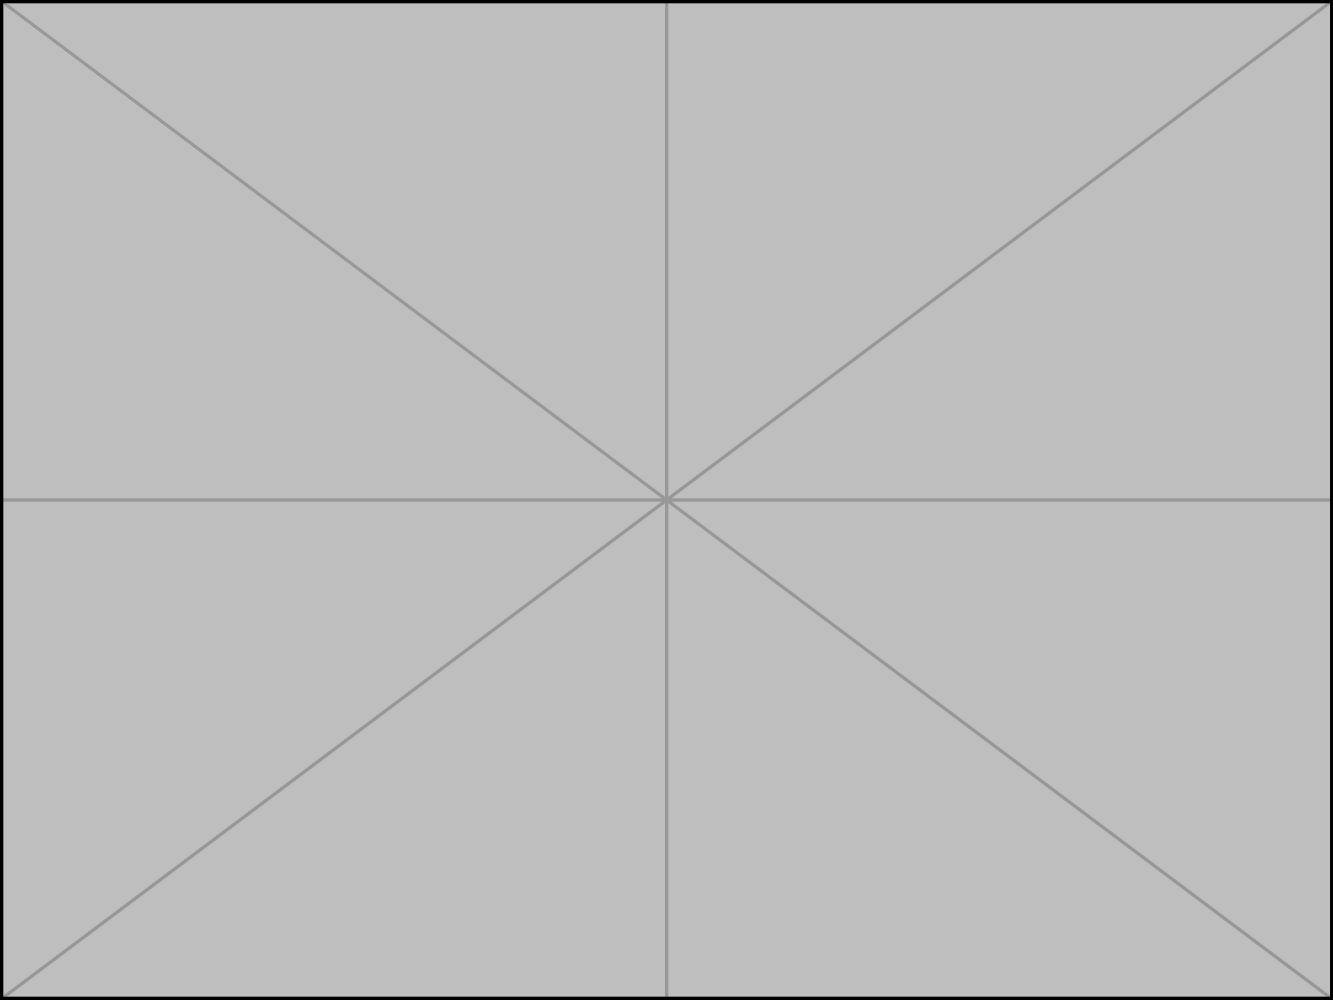
\includegraphics[width=2cm]{fig_image_vide.png}} & Protégé contre la poussière (pas de dépot nuisible)  	& 	& & & 5 & 	\adjustbox{valign=t}{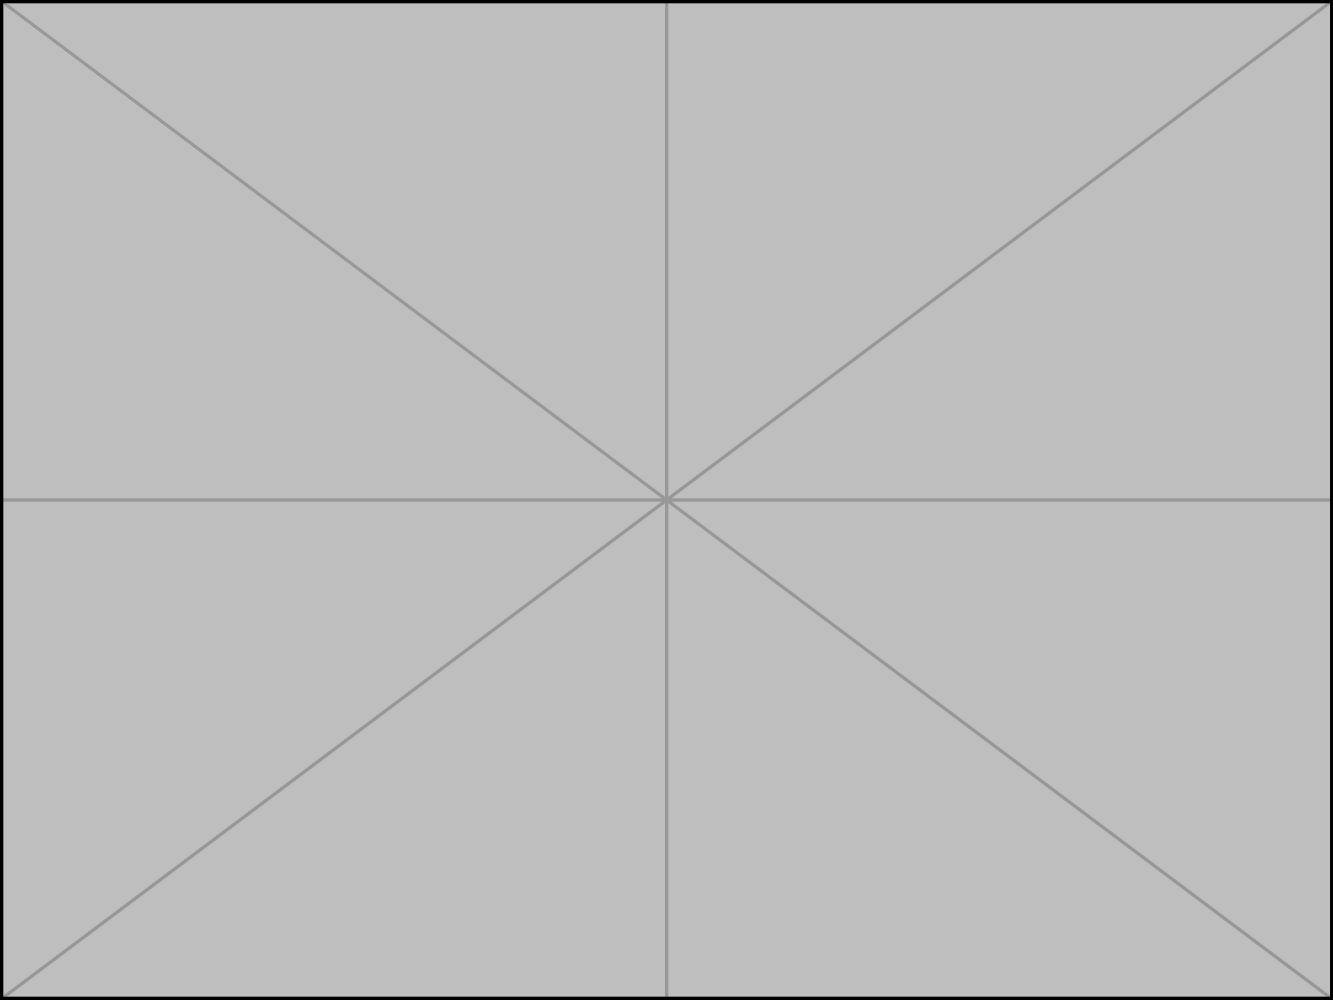
\includegraphics[width=2cm]{fig_image_vide.png}}	&	Protégé contre les jets d'eau dans toutes les directions à la lance \\
\addlinespace
6 		& \adjustbox{valign=t}{
\includegraphics[width=2cm]{fig_image.png}} & Totalement protégé contre la poussière 	& 	& & & 6 & 	\adjustbox{valign=t}{
\includegraphics[width=2cm]{fig_image.png}}	&	Protégé contre les projections d'eau assimilables aux paquets de mer \\
\addlinespace
 		&  & 	& 	& & & 7 & 	\adjustbox{valign=t}{
\includegraphics[width=2cm]{fig_image_a.png}}	&	Protégé contre les effets d'une immersion temporaire dans l'eau \\
 		\addlinespace
		&  & 	& 	& & & 8 & 	\adjustbox{valign=t}{
\includegraphics[width=2cm]{fig_image_b.png}}	&	Protégé contre les effets d'une immersion prolongée dans l'eau dans des conditions spécifiées \\
		\addlinespace
		&  & 	& 	& & & 9 & 	&	Protégé contre les jets d'eau haute pression et haute température mais pas nécessairement submersible \\
\end{longtableau}	
\end{landscape}
\end{minted}

Cela produira (tableau situé en dehors de l'environnement exemple pour des raisons de compatibilité) :\\


\end{exemple}


\begin{landscape}
    	\begin{TableNotes}
    \item[3] une troisième note en bas de tableau\,;
    \item[1000] une millième note en bas de tableau.
  \end{TableNotes}
  \begin{ThreePartTable}
\begin{longtableau}{\linewidth}{p{0.3cm} c X p{0.3cm} c X p{0.3cm} c X}{9}{Tableau à la largeur relative en paysage sur plusieurs pages, avec insertion de figures}
{\multicolumn{3}{c}{\thead{Protection contre les corps solides}}	& \multicolumn{3}{c}{\thead{Lettre additionnelle\\Contact direct avec les parties dangereuses}}	& \multicolumn{3}{c}{\thead{Protection contre les liquides}}}[\notetableau]
0 		& 									& Aucune protection	&	&	&	& 0 	&	&	Aucune protection \\
\addlinespace
1 		& \adjustbox{valign=t}{
\includegraphics[width=2cm]{fig_image.png}} & Protégé contre les corps solides \(\diameter \geq \SI{50}{\milli\meter}\)\tnote{3}  	&	A & \adjustbox{valign=t}{
\includegraphics[width=2cm]{fig_image.png}}	&	Le dos de la main reste éloigné des parties dangereuses.	& 1 & 	\adjustbox{valign=t}{
\includegraphics[width=2cm]{fig_image.png}}	&	Protégé contre les chutes verticales de gouttes d'eau (condensation) \\
\addlinespace
2 		& 	\adjustbox{valign=t}{
\includegraphics[width=2cm]{fig_image_a.png}} & Protégé contre les corps solides \(\diameter \geq \SI{12,5}{\milli\meter}\)  	& B	& \adjustbox{valign=t}{
\includegraphics[width=2cm]{fig_image_a.png}}	&	L'introduction d'un doigt ne permet pas de toucher les parties dangereuses. & 2 & 	\adjustbox{valign=t}{
\includegraphics[width=2cm]{fig_image_a.png}}	&	Protégé contre les chutes de gouttes d'eau jusqu'à 15° de la verticale \\
\addlinespace
3 		& 	\adjustbox{valign=t}{
\includegraphics[width=2cm]{fig_image_b.png}} & Protégé contre les corps solides \(\diameter \geq \SI{2,5}{\milli\meter}\)\tnote{1000} 	& C	& \adjustbox{valign=t}{
\includegraphics[width=2cm]{fig_image_b.png}}	&	L'introduction d'un outil ne permet pas de toucher les parties dangereuses. & 3 & 	\adjustbox{valign=t}{
\includegraphics[width=2cm]{fig_image_b.png}}	&	Protégé contre l'eau de pluie jusqu'à 60° de la verticale \\
\addlinespace
4 		& 	\adjustbox{valign=t}{
\includegraphics[width=2cm]{fig_image_c.png}} & Protégé contre les corps solides \(\diameter \geq \SI{1}{\milli\meter}\)  	& D	& \adjustbox{valign=t}{
\includegraphics[width=2cm]{fig_image_c.png}}	&	L'introduction d'un outil fin ne permet pas de toucher les parties dangereuses. & 4 & 	\adjustbox{valign=t}{
\includegraphics[width=2cm]{fig_image_c.png}}	&	Protégé contre les projections d'eau dans toutes les directions \\
\addlinespace
5 		& 	\adjustbox{valign=t}{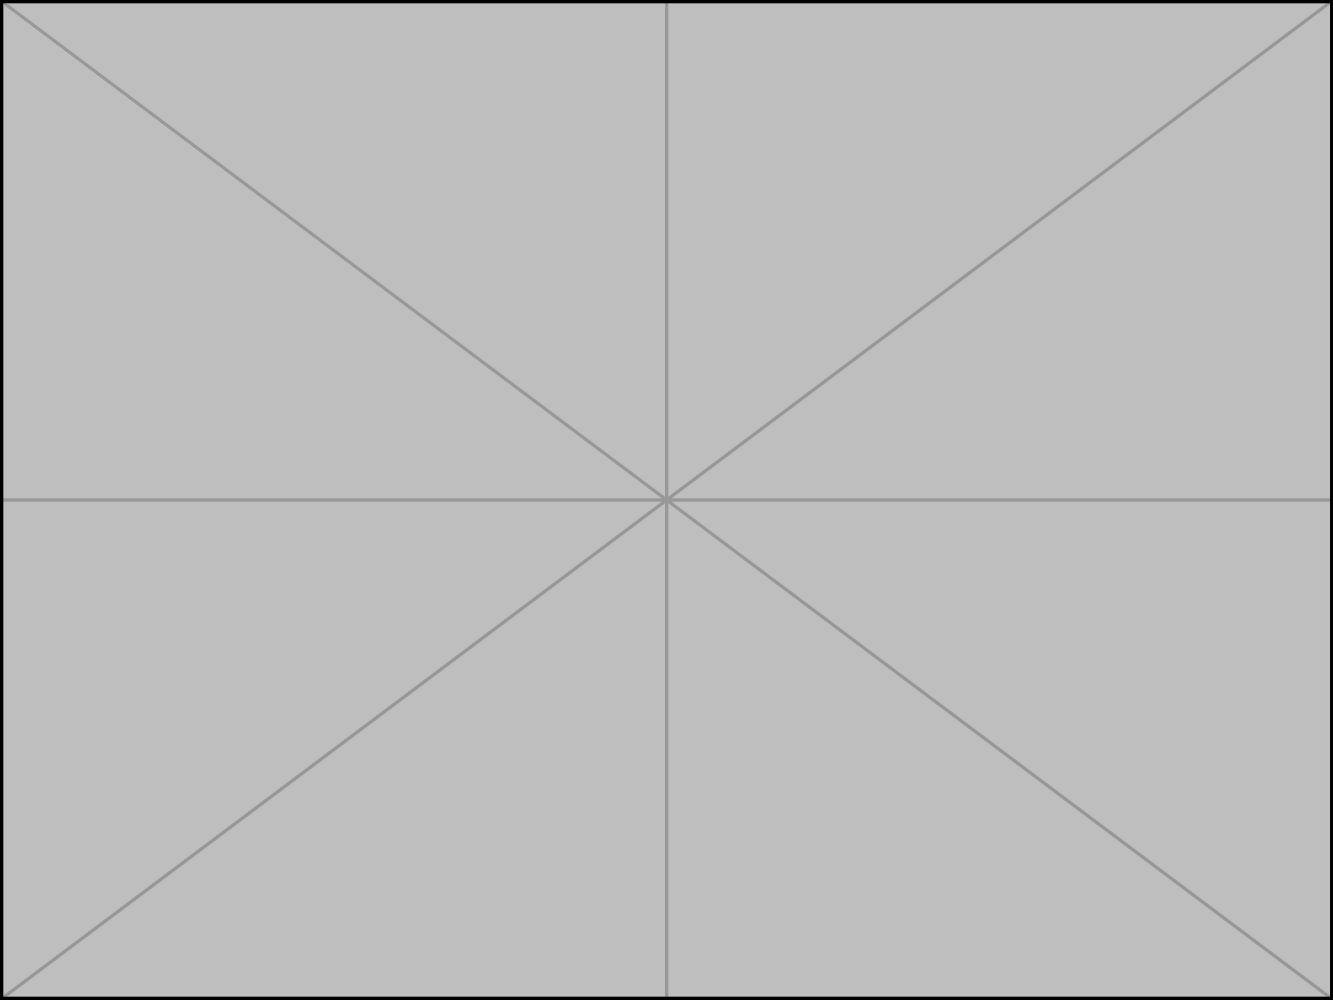
\includegraphics[width=2cm]{fig_image_vide.png}} & Protégé contre la poussière (pas de dépot nuisible)  	& 	& & & 5 & 	\adjustbox{valign=t}{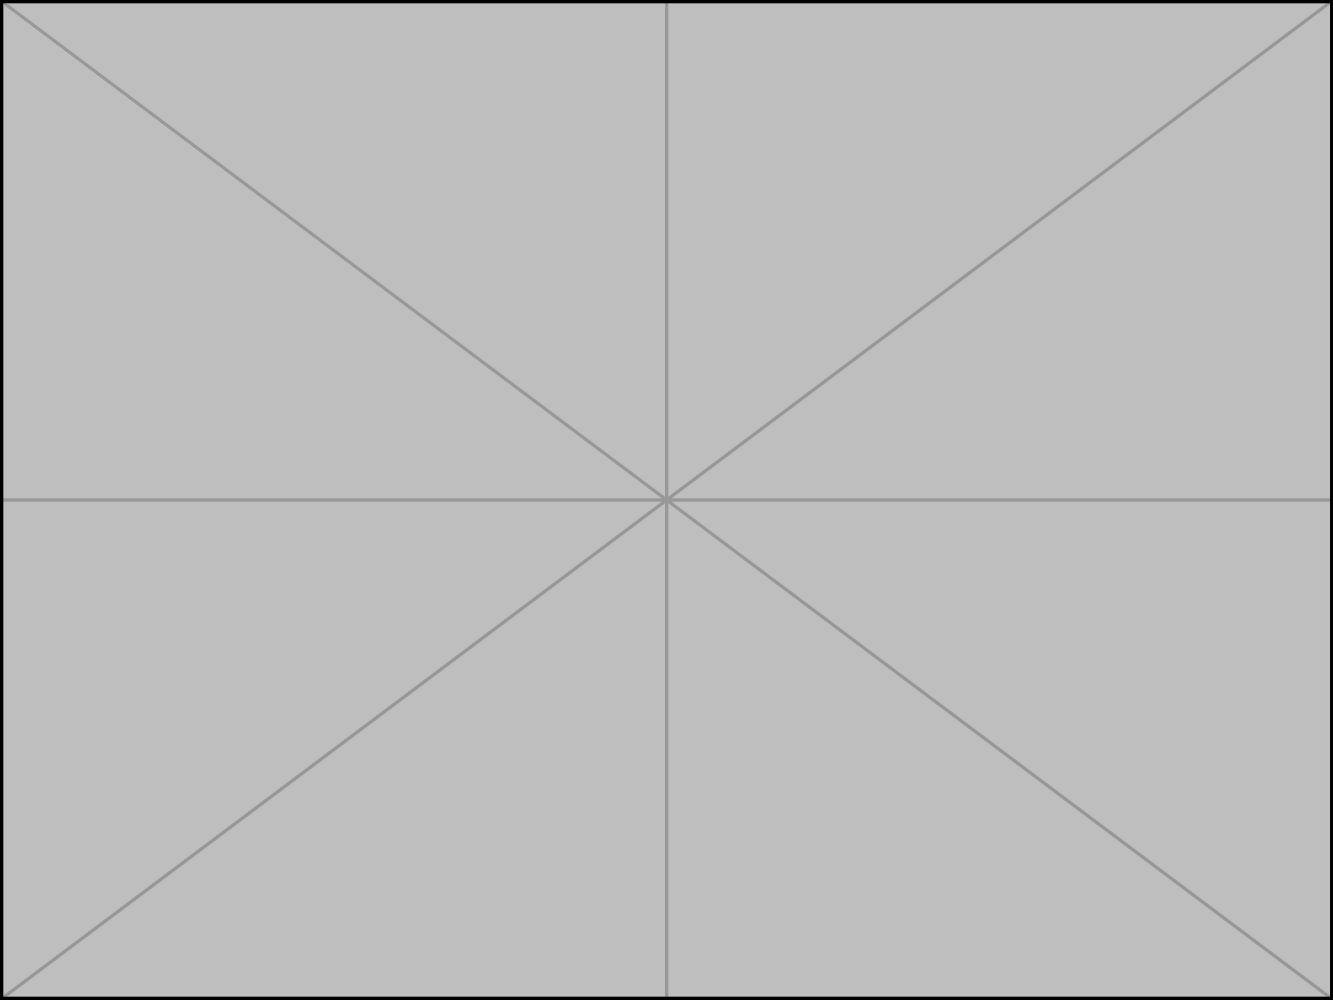
\includegraphics[width=2cm]{fig_image_vide.png}}	&	Protégé contre les jets d'eau dans toutes les directions à la lance \\
\addlinespace
6 		& \adjustbox{valign=t}{
\includegraphics[width=2cm]{fig_image.png}} & Totalement protégé contre la poussière 	& 	& & & 6 & 	\adjustbox{valign=t}{
\includegraphics[width=2cm]{fig_image.png}}	&	Protégé contre les projections d'eau assimilables aux paquets de mer \\
\addlinespace
 		&  & 	& 	& & & 7 & 	\adjustbox{valign=t}{
\includegraphics[width=2cm]{fig_image_a.png}}	&	Protégé contre les effets d'une immersion temporaire dans l'eau \\
 		\addlinespace
		&  & 	& 	& & & 8 & 	\adjustbox{valign=t}{
\includegraphics[width=2cm]{fig_image_b.png}}	&	Protégé contre les effets d'une immersion prolongée dans l'eau dans des conditions spécifiées \\
		\addlinespace
		&  & 	& 	& & & 9 & 	&	Protégé contre les jets d'eau haute pression et haute température mais pas nécessairement submersible \\
\end{longtableau}	
  \end{ThreePartTable}

\end{landscape}

\end{document}






%--------------------------------------
%conclusion, bibliographie
%--------------------------------------

\backmatter

	%--------------------------------------
	%inclusion des chapitres
	%--------------------------------------

	%--------------------------------------
	%bibliographie, glossaire et index
	%--------------------------------------
	
	\nocite{ISO:9001-2015}
	\printbibliography %ajout des références bibliographiques
	
	\printindex
	\printindex[exemple]
	
	\printnoidxglossary
	\printnoidxglossary[type=\acronymtype , title={Liste des acronymes}, toctitle={Liste des acronymes}]
		
\end{document}

